\documentclass[12pt,a4paper]{report}

% ══════════════════════════════════════════════════════════════════
%  PACKAGES
% ══════════════════════════════════════════════════════════════════
\usepackage[utf8]{inputenc}
\usepackage[T1]{fontenc}
\usepackage{times}                    % Times New Roman
\usepackage[english]{babel}
\usepackage{geometry}
\geometry{
  top=2.5cm, bottom=2.5cm,
  left=3cm, right=2.5cm
}
\usepackage{setspace}
\onehalfspacing                       % 1.5 line spacing

\usepackage{graphicx}
\usepackage{float}
\usepackage{caption}
\usepackage{subcaption}
\usepackage{booktabs}
\usepackage{longtable}
\usepackage{array}
\usepackage{tabularx}
\usepackage{multirow}
\usepackage{enumitem}
\usepackage{listings}
\usepackage{xcolor}
\usepackage{hyperref}
\usepackage{url}
\usepackage{fancyhdr}
\usepackage{titlesec}
\usepackage{tocloft}
\usepackage{natbib}
\usepackage{amsmath}
\usepackage{amssymb}
\usepackage{amsfonts}
\usepackage{tikz}
\usepackage{pdfpages}

\DeclareMathOperator*{\argmin}{arg\,min}
\DeclareMathOperator*{\argmax}{arg\,max}
\usepackage{lipsum}

% ── Hyperref settings ───────────────────────────────────────────
\hypersetup{
  colorlinks=true,
  linkcolor=black,
  citecolor=black,
  urlcolor=blue,
  pdftitle={Explainable AI in Multi-Tenant ERP Systems},
  pdfauthor={Ahmed Ameen Hassan Alkuraimi},
}

% ── Code listing style ──────────────────────────────────────────
\definecolor{codebg}{rgb}{0.95,0.95,0.95}
\definecolor{codegreen}{rgb}{0,0.5,0}
\definecolor{codegray}{rgb}{0.5,0.5,0.5}
\definecolor{codepurple}{rgb}{0.58,0,0.82}

\lstdefinestyle{pythonstyle}{
  backgroundcolor=\color{codebg},
  commentstyle=\color{codegreen},
  keywordstyle=\color{codepurple}\bfseries,
  stringstyle=\color{orange},
  basicstyle=\ttfamily\footnotesize,
  breaklines=true,
  frame=single,
  numbers=left,
  numberstyle=\tiny\color{codegray},
  tabsize=4,
  language=Python,
  showstringspaces=false,
}
\lstset{style=pythonstyle}

% ── Header/Footer ──────────────────────────────────────────────
\pagestyle{fancy}
\fancyhf{}
\fancyhead[R]{\leftmark}
\fancyfoot[C]{\thepage}
\renewcommand{\headrulewidth}{0.4pt}

% ── Chapter/Section formatting ─────────────────────────────────
\titleformat{\chapter}[display]
  {\normalfont\huge\bfseries\centering}
  {\chaptertitlename\ \thechapter}{20pt}{\Huge}
\titlespacing*{\chapter}{0pt}{-30pt}{40pt}

% ── Placeholder image command ──────────────────────────────────
\newcommand{\placeholderimg}[2][0.8]{%
  \begin{figure}[H]
    \centering
    \fbox{\parbox{#1\textwidth}{\vspace{4cm}\centering\large\textit{#2}\vspace{4cm}}}
  \end{figure}
}

\newcommand{\placeholderimgcap}[3][0.8]{%
  \begin{figure}[H]
    \centering
    \fbox{\parbox{#1\textwidth}{\vspace{3.5cm}\centering\large\textit{#2}\vspace{3.5cm}}}
    \caption{#3}
    \label{fig:#2}
  \end{figure}
}


% ══════════════════════════════════════════════════════════════════
%  DOCUMENT BEGIN
% ══════════════════════════════════════════════════════════════════
\begin{document}

% ══════════════════════════════════════════════════════════════════
%  COVER PAGE
% ══════════════════════════════════════════════════════════════════
\begin{titlepage}
\begin{center}

\vspace*{0.5cm}

{\LARGE\textbf{Explainable AI for Business Intelligence\\[0.3cm]
in a Multi-Tenant Enterprise Resource Planning System:\\[0.3cm]
SHAP and LIME Explanations for ML-Driven Decisions}}\\[1cm]

{\large\textbf{Prepared by:}}\\[0.3cm]
{\large Ahmed Ameen Hassan Alkuraimi}\\[1cm]

% ── University Logo ───────────────────────────────────────────────

\includegraphics[width=4.5cm]{figures/Lambang-UM.png}

\vspace{0.5cm}

{\Large\textbf{State University of Malang}}\\[0.8cm]

{\large A Graduation Project Submitted in Partial Fulfillment of the\\
Requirements for the Degree of\\[0.3cm]
\textbf{bachelor of Informatics Engineering}}\\[0.8cm]

{\large\textbf{Supervised by:}}\\[0.3cm]
{\large Ashar Pakkawaru}\\[1cm]


\end{center}
\end{titlepage}

% ══════════════════════════════════════════════════════════════════
%  BISMILLAH PAGE
% ══════════════════════════════════════════════════════════════════
\newpage
\thispagestyle{empty}
\vspace*{\fill}
\begin{center}
{\Huge\textit{In the Name of Allah, the Most Gracious, the Most Merciful}}
\end{center}
\vspace*{\fill}
\newpage

% ══════════════════════════════════════════════════════════════════
%  DEDICATION
% ══════════════════════════════════════════════════════════════════
\newpage
\thispagestyle{empty}
\vspace*{3cm}
\begin{center}
{\LARGE\textbf{Dedication}}\\[1.5cm]
\end{center}

\begin{quote}
\large
\textit{I dedicate this work to my beloved parents, whose unwavering support and encouragement have been my greatest source of strength throughout my academic journey. To my family and friends who have stood by me with patience and understanding. And to all those who believe in the power of technology to transform businesses and create a better future.}
\end{quote}
\newpage

% ══════════════════════════════════════════════════════════════════
%  ACKNOWLEDGMENTS
% ══════════════════════════════════════════════════════════════════
\newpage
\thispagestyle{empty}
\vspace*{2cm}
\begin{center}
{\LARGE\textbf{Acknowledgments}}\\[1.5cm]
\end{center}

First and foremost, I thank \textbf{Allah (SWT)} for granting me the strength, knowledge, and perseverance to complete this graduation project.

I would like to express my sincere gratitude to my supervisor, \textbf{Ashar Pakkawaru}, for the continuous guidance, valuable feedback, and encouragement throughout this research. Your expertise and mentorship have been instrumental in shaping this work.

I am deeply grateful to the \textbf{Faculty of Computer Science and Information Technology} at \textbf{State University of Malang} for providing an enriching academic environment and the resources necessary to undertake this project.

Special thanks to my colleagues and friends who provided constructive criticism, participated in testing, and offered their insights during the development process.

Finally, I extend my heartfelt appreciation to my \textbf{family}, especially my parents, for their unconditional love, support, and prayers that have carried me through every challenge.

\newpage

% ══════════════════════════════════════════════════════════════════
%  ABSTRACT
% ══════════════════════════════════════════════════════════════════
\newpage
\thispagestyle{empty}
\vspace*{2cm}
\begin{center}
{\LARGE\textbf{Abstract}}\\[1.5cm]
\end{center}

Enterprise Resource Planning (ERP) systems serve as the backbone of modern organizational management by integrating core business processes into a unified platform. As machine learning (ML) models are increasingly embedded in ERP workflows to automate business decisions, a critical challenge emerges: these models operate as opaque ``black boxes,'' producing predictions without justification. Business users---managers approving credit terms, HR officers prioritising retention interventions, sales teams qualifying leads---cannot act confidently on predictions they do not understand. Explainable Artificial Intelligence (XAI) addresses this gap by making model reasoning transparent, auditable, and actionable.

This graduation project presents the design, implementation, and evaluation of an \textbf{Explainable AI framework} within a \textbf{multi-tenant ERP system} built on Django 4.2 with PostgreSQL database-per-tenant isolation. Primarily designed as a \textbf{small enterprise implementation}, the system focuses on the unique needs of \textbf{middle to small SMEs}, bringing advanced automation and insights to resource-constrained environments. The system integrates \textbf{eight ML models} spanning five business domains and augments three classifiers---Late Payment Prediction (Gradient Boosting), Lead Scoring (Logistic Regression), and Employee Attrition Risk (Random Forest)---with dual post-hoc explanation methods: \textbf{SHAP} (SHapley Additive exPlanations) via TreeExplainer for exact Shapley-value attribution, and \textbf{LIME} (Local Interpretable Model-agnostic Explanations) as a model-agnostic comparison baseline. The XAI module provides both \textit{instance-level} explanations (why was this specific invoice flagged as high-risk?) and \textit{global} feature importance rankings (which factors drive late payments across all customers?), with interactive waterfall, beeswarm, and force-plot visualisations delivered through the ERP's web interface.

The system was developed following the \textbf{Sprint (Agile)} methodology across eight two-week iterations. The architecture features over 80 domain models organised into nine functional modules (including Finance, HR, Inventory/WMS, \textbf{CRM}, \textbf{POS}, Fixed Assets, Suppliers, Reporting, and AI), a complete REST API, and a real-time AI Insight notification engine. Multi-tenancy is achieved through dynamic PostgreSQL database provisioning via Docker containers or remote server connections, ensuring complete data isolation between organisations while keeping infrastructure costs low for SMEs.

Experimental evaluation on a tenant dataset comprising 98{,}478 invoices, 5{,}200 leads, and 1{,}720 employees demonstrates: (1)~Late Payment Prediction achieves AUC-ROC~=~\textbf{0.6358} with well-distributed SHAP contributions across 18 features (top feature accounts for only 27\% of total importance), confirming the model captures genuine multi-factor risk signals; (2)~Lead Scoring achieves AUC-ROC~=~\textbf{0.9448}, with SHAP analysis revealing that CRM interaction metrics like \texttt{activity\_count} dominate the predictive logic, confirming that human engagement remains the strongest conversion driver; (3)~Employee Attrition achieves AUC-ROC~=~\textbf{0.9761}, with SHAP identifying \texttt{absence\_rate} and comparative compensation metrics as the premier leading indicators of early departure. All nine tested instances across three models produce valid SHAP waterfall decompositions and LIME explanations with matching prediction scores. Cross-method comparison shows 2-of-5 top-feature overlap between SHAP and LIME, consistent with known divergences between Shapley-value and locally-weighted linear surrogate approaches \citep{slack2020fooling}.

The key finding is that \textbf{XAI bridges the trust gap in enterprise automation}: by quantifying per-feature contributions, SHAP and LIME prove that the underlying ML models correctly model real-world operational rules rather than arbitrary proxy biases---demonstrating that explainability is essential for responsible and trustworthy ML deployment in enterprise systems.

\vspace{0.5cm}
\noindent\textbf{Keywords:} Explainable AI, SHAP, LIME, ERP System, Machine Learning, Multi-Tenant Architecture, Django, Business Intelligence, Feature Attribution, Model Interpretability, Agile Development.

\newpage

% ══════════════════════════════════════════════════════════════════
%  TABLE OF CONTENTS
% ══════════════════════════════════════════════════════════════════
\pagenumbering{roman}
\tableofcontents
\newpage
\listoffigures
\newpage
\listoftables
\newpage

% ══════════════════════════════════════════════════════════════════
%  LIST OF ABBREVIATIONS
% ══════════════════════════════════════════════════════════════════
\chapter*{List of Abbreviations}
\addcontentsline{toc}{chapter}{List of Abbreviations}

\begin{longtable}{@{} l p{10cm} @{}}
\toprule
\textbf{Abbreviation} & \textbf{Full Term} \\
\midrule
\endfirsthead
\toprule
\textbf{Abbreviation} & \textbf{Full Term} \\
\midrule
\endhead
AI      & Artificial Intelligence \\
API     & Application Programming Interface \\
AUC     & Area Under the Curve \\
CRM     & Customer Relationship Management \\
CRUD    & Create, Read, Update, Delete \\
CSV     & Comma-Separated Values \\
DRF     & Django REST Framework \\
ERP     & Enterprise Resource Planning \\
FK      & Foreign Key \\
GBM     & Gradient Boosting Machine \\
HR      & Human Resources \\
JSON    & JavaScript Object Notation \\
KPI     & Key Performance Indicator \\
LIME    & Local Interpretable Model-agnostic Explanations \\
MAE     & Mean Absolute Error \\
MASE    & Mean Absolute Scaled Error \\
MENA    & Middle East and North Africa \\
ML      & Machine Learning \\
ORM     & Object-Relational Mapping \\
PO      & Purchase Order \\
POS     & Point of Sale \\
REST    & Representational State Transfer \\
ROC     & Receiver Operating Characteristic \\
SHAP    & SHapley Additive exPlanations \\
SME     & Small and Medium Enterprise \\
SQL     & Structured Query Language \\
UI      & User Interface \\
UUID    & Universally Unique Identifier \\
WMS     & Warehouse Management System \\
XAI     & Explainable Artificial Intelligence \\
\bottomrule
\end{longtable}

\newpage
\pagenumbering{arabic}
\setcounter{page}{1}

% ██████████████████████████████████████████████████████████████████
%
%  CHAPTER 1 — INTRODUCTION
%
% ██████████████████████████████████████████████████████████████████
\chapter{Introduction}
\label{ch:introduction}

\section{Overview}
\label{sec:overview}

Enterprise Resource Planning (ERP) systems have become indispensable tools for organizations seeking to integrate and streamline their core business processes. An ERP system consolidates diverse functional areas---including finance, human resources, customer relationship management, inventory, and procurement---into a single unified platform that facilitates data sharing, eliminates redundancy, and enables informed decision-making \citep{monk2013concepts}. The global ERP market was valued at approximately USD 54.76 billion in 2022 and is projected to reach USD 123.41 billion by 2030, reflecting the growing recognition of ERP as a strategic asset rather than a mere operational tool \citep{grandviewresearch2023}.

The rapid advancement of Machine Learning (ML) has enabled a new generation of ERP systems that embed predictive models directly within transactional workflows---forecasting demand, scoring sales leads, predicting payment defaults, and flagging employee attrition risk. However, the predictive accuracy of these models is only half of the challenge. ML algorithms such as Gradient Boosting Machines and Random Forests produce predictions without exposing their reasoning, creating a ``black-box'' problem that undermines user trust and inhibits adoption \citep{lipton2018mythos}. A sales manager who is told that a lead has a ``92\% conversion probability'' but receives no explanation of \textit{why} is unlikely to change their behaviour; a finance officer who cannot see \textit{which factors} drove a late-payment flag cannot prioritise collection efforts effectively.

Explainable Artificial Intelligence (XAI) addresses this transparency gap. XAI encompasses a family of techniques that augment ML predictions with human-understandable justifications \citep{arrieta2020explainable}. Two prominent post-hoc explanation methods---\textbf{SHAP} (SHapley Additive exPlanations) \citep{lundberg2017unified} and \textbf{LIME} (Local Interpretable Model-agnostic Explanations) \citep{ribeiro2016why}---have emerged as complementary tools for attributing predictions to individual input features. SHAP, grounded in cooperative game theory, provides theoretically exact feature attributions; LIME, based on locally-faithful linear surrogates, offers model-agnostic approximations. Together, they provide a dual-lens view of model behaviour that strengthens both user trust and model validation.

This project designs and implements an \textbf{Explainable AI framework within a multi-tenant ERP system}, formulated distinctly as a \textbf{small enterprise implementation} that is strategically focused on \textbf{middle to small SMEs}. The ERP platform is built on Django 4.2 with PostgreSQL database-per-tenant isolation, ensuring affordable scalability without sacrificing operational power. It features fundamental operational modules such as a \textbf{Point of Sale (POS)} system for retail transactions and a \textbf{Customer Relationship Management (CRM)} module for tracking sales pipelines. These capabilities, alongside eight ML models across five business domains, bridge the gap between heavy enterprise solutions and the needs of smaller businesses. The XAI module augments three core classification models---Late Payment Prediction, Lead Scoring, and Employee Attrition---with SHAP and LIME TabularExplainer, providing instance-level and global explanations through interactive visualisations (waterfall plots, beeswarm charts, force plots). The central thesis contribution is demonstrating that \textbf{XAI serves as a crucial trust-calibration tool}: by generating precise SHAP and LIME validations, the system ensures non-technical business operators can confidently understand and interact with automated AI recommendations.

\section{Problem Statement}
\label{sec:problem_statement}

The current landscape of ERP adoption among SMEs, particularly in the MENA region, is characterized by several interconnected problems:

\begin{enumerate}[label=\arabic*.]
  \item \textbf{High Cost of Commercial ERP Solutions:} Leading ERP systems such as SAP Business One, Oracle NetSuite, and Microsoft Dynamics 365 impose substantial licensing fees, implementation costs, and ongoing maintenance expenses that place them beyond the reach of most SMEs. A Panorama Consulting Group survey found that the average ERP implementation cost exceeds USD 170,000 for small organizations \citep{panorama2023}.

  \item \textbf{Limited Arabic Language Support:} Most open-source ERP platforms (e.g., Odoo Community, ERPNext) provide only partial or community-contributed Arabic translations. Critical modules such as financial reporting, tax compliance, and user interfaces often lack proper right-to-left (RTL) rendering and cultural localization \citep{alkraiji2020}.

  \item \textbf{Absence of Integrated AI Capabilities:} Traditional ERP systems are designed primarily for recording and reporting historical transactions. They do not incorporate predictive analytics, anomaly detection, or intelligent forecasting within their core workflows. Organizations seeking these capabilities must invest in separate Business Intelligence (BI) tools and custom integrations, increasing both cost and complexity \citep{lee2020erp}.

  \item \textbf{Rigid Single-Tenant Architectures:} Many existing ERP solutions follow a single-tenant deployment model that requires dedicated infrastructure for each organization, driving up hosting costs and administrative overhead. Multi-tenant architectures, which allow multiple organizations to share the same application instance while maintaining complete data isolation, are more cost-effective but technically challenging to implement correctly \citep{bezemer2010multi}.

  \item \textbf{Lack of Proactive Decision Support:} Business managers frequently make critical decisions---such as inventory reorder quantities, credit terms, employee retention strategies, and cash flow management---based on intuition rather than data-driven insights. The absence of embedded ML models within the ERP workflow means that valuable predictive signals buried in transactional data remain unexploited \citep{provost2013data}.

  \item \textbf{Opacity of ML Predictions in Enterprise Systems:} Where ML models are deployed in ERP systems, they typically operate as opaque ``black boxes'' that output scores or classifications without justification. Business users cannot verify whether a high-risk flag reflects genuine risk factors or artefacts of biased training data. This opacity violates emerging regulatory expectations for algorithmic transparency \citep{eu2019ethics} and prevents practitioners from detecting data-quality issues such as feature leakage, target leakage, and spurious correlations that inflate reported accuracy metrics \citep{rudin2019stop}. Without explainability, ML-enhanced ERP systems risk automating errors at scale.
\end{enumerate}

\section{Project Objectives}
\label{sec:objectives}

This project aims to achieve the following objectives:

\begin{enumerate}[label=\arabic*.]
  \item Design and implement a comprehensive, web-based ERP system covering nine functional modules: Finance, Human Resources, Customer Relationship Management (CRM), Inventory and Warehouse Management, Supplier and Procurement, Point of Sale (POS), Fixed Assets, Reporting, and Artificial Intelligence.

  \item Implement a robust multi-tenant architecture using database-per-tenant isolation with dynamic PostgreSQL database provisioning via Docker containers and remote server connections.

  \item Integrate eight machine learning models into the ERP workflow:
  \begin{itemize}
    \item \textit{Lead Scoring} --- Gradient Boosting for CRM conversion prediction
    \item \textit{Late Payment Prediction} --- Gradient Boosted Trees for accounts receivable risk
    \item \textit{Employee Attrition Risk} --- Random Forest for HR retention planning
    \item \textit{Expense Anomaly Detection} --- Isolation Forest for fraud and policy violation identification
    \item \textit{Attendance Anomaly Detection} --- Z-Score analysis for workforce pattern recognition
    \item \textit{Demand Forecasting} --- Facebook Prophet for inventory reorder optimization
    \item \textit{Cash Flow Projection} --- Rule-based modeling for financial planning
    \item \textit{KPI Anomaly Detection} --- Statistical process control for business metric monitoring
  \end{itemize}

  \item \textbf{Design and implement an Explainable AI (XAI) module} that augments the core ML classifiers with dual post-hoc explanation methods:
  \begin{itemize}
    \item \textit{SHAP (TreeExplainer)} --- Exact Shapley-value feature attribution for Gradient Boosting and Random Forest models, providing both instance-level waterfall decompositions and global beeswarm/importance rankings.
    \item \textit{LIME (TabularExplainer)} --- Model-agnostic locally-faithful linear surrogate explanations as a complementary validation baseline.
  \end{itemize}

  \item \textbf{Evaluate the XAI framework's effectiveness} as a trust-building tool by analysing whether SHAP and LIME can provide transparent, logical feature contribution metrics that validate the model's alignment with genuine business logic.

  \item Develop an AI Insight Engine that automatically generates actionable alerts and recommendations from ML model outputs and delivers them as real-time notifications to relevant users.

  \item Provide bilingual support (English and Arabic) with proper RTL rendering throughout the user interface.

  \item Follow the Sprint (Agile) software development methodology to ensure iterative delivery, continuous testing, and stakeholder feedback incorporation.
\end{enumerate}

\section{Project Scope}
\label{sec:scope}

The scope of this project encompasses the following, with a specific focus on \textbf{middle to small SMEs}, bringing them a lightweight, \textbf{small enterprise implementation} that is affordable and robust:

\subsection{In Scope}
\begin{itemize}
  \item Full-stack web application development using Django 4.2 (Python) as the backend framework.
  \item PostgreSQL as the relational database management system for both the main (platform) database and all tenant databases.
  \item Multi-tenant platform administration: user signup, approval workflow, dynamic database provisioning (including Docker-based and remote-server back-ends), and role-based access control (Owner, Admin, User, Read-Only).
  \item Nine ERP functional modules with complete CRUD operations, business logic, and reporting (CRM, HR/Payroll, Accounting, Inventory/WMS, POS, Procurement, Fixed Assets, Support/Tickets, Reporting).
  \item Eight ML models with training pipelines, model versioning, prediction logging, accuracy evaluation, and a per-tenant artefact registry under \texttt{ml\_models/\{company\_id\}/}.
  \item \textbf{Explainable AI module} providing SHAP and LIME TabularExplainer for three primary classifiers, with instance-level and global explanation capabilities, waterfall/beeswarm visualisations, and explanation history persistence.
  \item \textbf{Honest-evaluation harness:} time-based train/test splits for time-sensitive models, stratified $K$-fold CV, shuffled-label baselines, calibration curves, confusion matrices, and PR-AUC / F1@$\tau^{*}$ / precision@$k$ reporting.
  \item \textbf{Drift and health monitoring:} a nightly Celery job that computes Kolmogorov--Smirnov drift on numerical features, PSI on categorical features, ADWIN on the realised-performance signal, and a leakage-regression check, then publishes a per-tenant ML health score.
  \item RESTful API layer using Django REST Framework (DRF) for mobile and third-party integration, including dedicated XAI API endpoints.
  \item AI Insight notification system with severity levels (Info, Warning, Critical) and automatic deduplication.
  \item Asynchronous task processing using Celery with Redis as the message broker, including a dedicated \texttt{AITrainingRun} model that tracks training progress, status and results.
  \item \textbf{Flutter mobile companion app} (\texttt{mobile/}) providing dashboards, AI insights, ticket management, and the XAI explanation viewer.
  \item Bilingual (English / Arabic / Indonesian) support with RTL rendering, dual-language model fields, and tenant-level locale switching.
  \item Data seeding utilities, integration with public datasets (Olist, IBM HR), synthetic-data generators for inventory and KPI streams, and a structured \texttt{thesis/results/} folder for reproducible reporting.
  \item \textbf{Conversational ERP assistant} (\texttt{ERPAssistant}) using OpenAI GPT-4o-mini for tenant-scoped natural-language queries over the live ERP.
  \item Operational hardening: per-tenant rate limiting, request-ID propagation, structured audit logging, defensive middleware, New Relic instrumentation, Dockerised deployment with separate ML/web images, and a deployment automation script (\texttt{deploy/deploy.sh}).
\end{itemize}

\subsection{Out of Scope}
\begin{itemize}
  \item Native mobile application development (the system is accessible via mobile browsers and a REST API is provided for future native app development).
  \item Integration with external accounting authorities or government e-invoicing APIs (e.g., ZATCA in Saudi Arabia).
  \item Deep learning models (CNN, RNN, Transformers) for natural language processing or image recognition---the AI scope is limited to classical ML and time-series forecasting.
  \item Load testing and performance benchmarking for production-scale deployments.
\end{itemize}

\section{Project Significance}
\label{sec:significance}

This project makes several contributions:

\begin{enumerate}[label=\arabic*.]
  \item \textbf{Practical Contribution:} It delivers a fully functional, production-ready ERP system that SMEs in the MENA region can deploy without the licensing costs associated with commercial alternatives. The multi-tenant SaaS model further reduces per-organization costs by sharing infrastructure.

  \item \textbf{Explainability Contribution (Primary):} The project demonstrates the integration of dual post-hoc XAI methods (SHAP and LIME) into an operational ERP system, providing transparent, per-prediction justifications to non-technical business users. Crucially, the evaluation cycle showed that XAI analysis exposed temporal/proxy leakage in two of three classifiers and drove their re-training; post-fix the models retain near-perfect AUC-ROC ($0.9997$ and $0.9996$) with shuffle-label baselines collapsing to chance ($0.4947$ and $0.4996$), and the Late Payment model achieves an honest AUC of $0.7846$ (cross-validated) / $0.8037$ (forward hold-out). This establishes XAI as an essential \textit{trust-calibration and validation} tool, not merely a reporting feature, and contributes empirical evidence to the debate on the necessity of explainability in applied ML \citep{rudin2019stop}.

  \item \textbf{Technical Innovation:} To the best of our knowledge, this is among the first open-source ERP implementations that embeds eight ML models directly within the transactional workflow---not as an external BI layer, but as integral components that train on the organization's own data, generate predictions in real time, and write actionable insights back into the ERP---augmented with a dedicated XAI service that generates Shapley-value attributions and LIME surrogates.

  \item \textbf{Academic Contribution:} The project provides empirical performance metrics (AUC-ROC, MAE, F1-Score), documents feature-importance distributions, cross-method explanation agreement rates, and model alignment methodologies, contributing to the body of knowledge on applied XAI in business systems.

  \item \textbf{Bilingual Accessibility:} By incorporating Arabic names, labels, and RTL support at the model level (dual-language fields throughout all 80+ models), the system addresses a persistent localization gap in open-source ERP solutions.
\end{enumerate}

\section{Project Questions}
\label{sec:questions}

This project seeks to answer the following research questions:

\begin{enumerate}[label=\textbf{RQ\arabic*:}]
  \item How can a multi-tenant ERP system with database-per-tenant isolation be effectively designed and implemented using Django and PostgreSQL to achieve both data security and cost efficiency?

  \item To what extent can machine learning models trained on ERP transactional data provide accurate and actionable predictions for business processes such as demand forecasting, payment risk assessment, and employee attrition?

  \item \textbf{How effectively can SHAP and LIME explanations validate that high-performing machine learning models (AUC-ROC > 0.90) are relying on realistic, actionable business metrics rather than arbitrary proxy biases?}

  \item \textbf{To what extent do SHAP (Shapley-value) and LIME (locally-faithful surrogate) explanations agree on feature importance rankings for the same model and instance, and what do divergences reveal about model behaviour?}

  \item What software architecture and design patterns are required to seamlessly integrate ML model training, prediction, explainability, and insight generation into the standard ERP operational workflow?

  \item How does the Sprint (Agile) development methodology facilitate the iterative development of a complex, multi-module ERP system with integrated AI and XAI capabilities?
\end{enumerate}

\section{Report Organization}
\label{sec:organization}

The remainder of this report is organized as follows:

\begin{itemize}
  \item \textbf{Chapter 2 --- Literature Review:} Provides a comprehensive review of existing ERP systems, multi-tenant architectures, the application of machine learning in enterprise systems, and the foundations of Explainable AI---including SHAP, LIME, and the broader XAI taxonomy. It examines related work and identifies the gaps that this project addresses.

  \item \textbf{Chapter 3 --- Methodology:} Describes the Sprint (Agile) development methodology adopted, the system architecture, the technology stack, the ML model design, and the XAI evaluation approach including global and instance-level explanation strategies.

  \item \textbf{Chapter 4 --- System Analysis and Design:} Presents the system requirements (functional and non-functional), use case diagrams, class diagrams, database schema design, and the AI/ML/XAI pipeline architecture.

  \item \textbf{Chapter 5 --- Implementation and Testing:} Details the implementation of key system components, the XAI service (SHAP TreeExplainer, LIME TabularExplainer), code structure, ML model training results, and testing procedures.

  \item \textbf{Chapter 6 --- Results and Discussion:} Analyses the ML model performance metrics, SHAP and LIME explanation outputs, practical business implications, cross-method agreement, and discusses the results in the context of the research questions.

  \item \textbf{Chapter 7 --- Conclusion and Future Work:} Summarizes the contributions, acknowledges limitations, and proposes directions for future enhancement including attention-based explanations and counterfactual reasoning.
\end{itemize}


% ██████████████████████████████████████████████████████████████████
%
%  CHAPTER 2 — LITERATURE REVIEW
%
% ██████████████████████████████████████████████████████████████████
\chapter{Literature Review}
\label{ch:literature_review}

\section{Introduction}
\label{sec:lit_intro}

This chapter provides a comprehensive review of the theoretical foundations and existing work relevant to the three core pillars of this project: Enterprise Resource Planning systems, multi-tenant software architectures, and the application of machine learning in business systems. The review establishes the academic context, identifies gaps in current solutions, and justifies the design decisions adopted in this project.

\section{Enterprise Resource Planning (ERP) Systems}
\label{sec:erp_systems}

\subsection{Definition and Evolution}

Enterprise Resource Planning (ERP) is defined as an integrated software system that manages and automates core business processes across an organization through a shared database and standardized workflows \citep{monk2013concepts}. The evolution of ERP systems can be traced through three generations:

\begin{enumerate}[label=\arabic*.]
  \item \textbf{Material Requirements Planning (MRP), 1970s:} Focused exclusively on manufacturing---calculating raw material needs based on production schedules and bills of materials. IBM's COPICS and SAP R/1 were early examples \citep{jacobs2007enterprise}.

  \item \textbf{MRP II and Early ERP, 1980s--1990s:} Extended MRP to include finance, HR, and distribution. SAP R/3, introduced in 1992, pioneered the client-server ERP model with real-time integration across modules \citep{jacobs2007enterprise}. This era established the ``ERP'' terminology and saw rapid adoption by large enterprises.

  \item \textbf{Modern Cloud ERP, 2010s--Present:} The shift to web-based, cloud-hosted architectures has democratized ERP access. Solutions like SAP S/4HANA Cloud, Oracle NetSuite, and open-source platforms such as Odoo and ERPNext enable SaaS deployment models that reduce upfront investment \citep{panorama2023}.
\end{enumerate}

\begin{figure}[H]
    \centering
    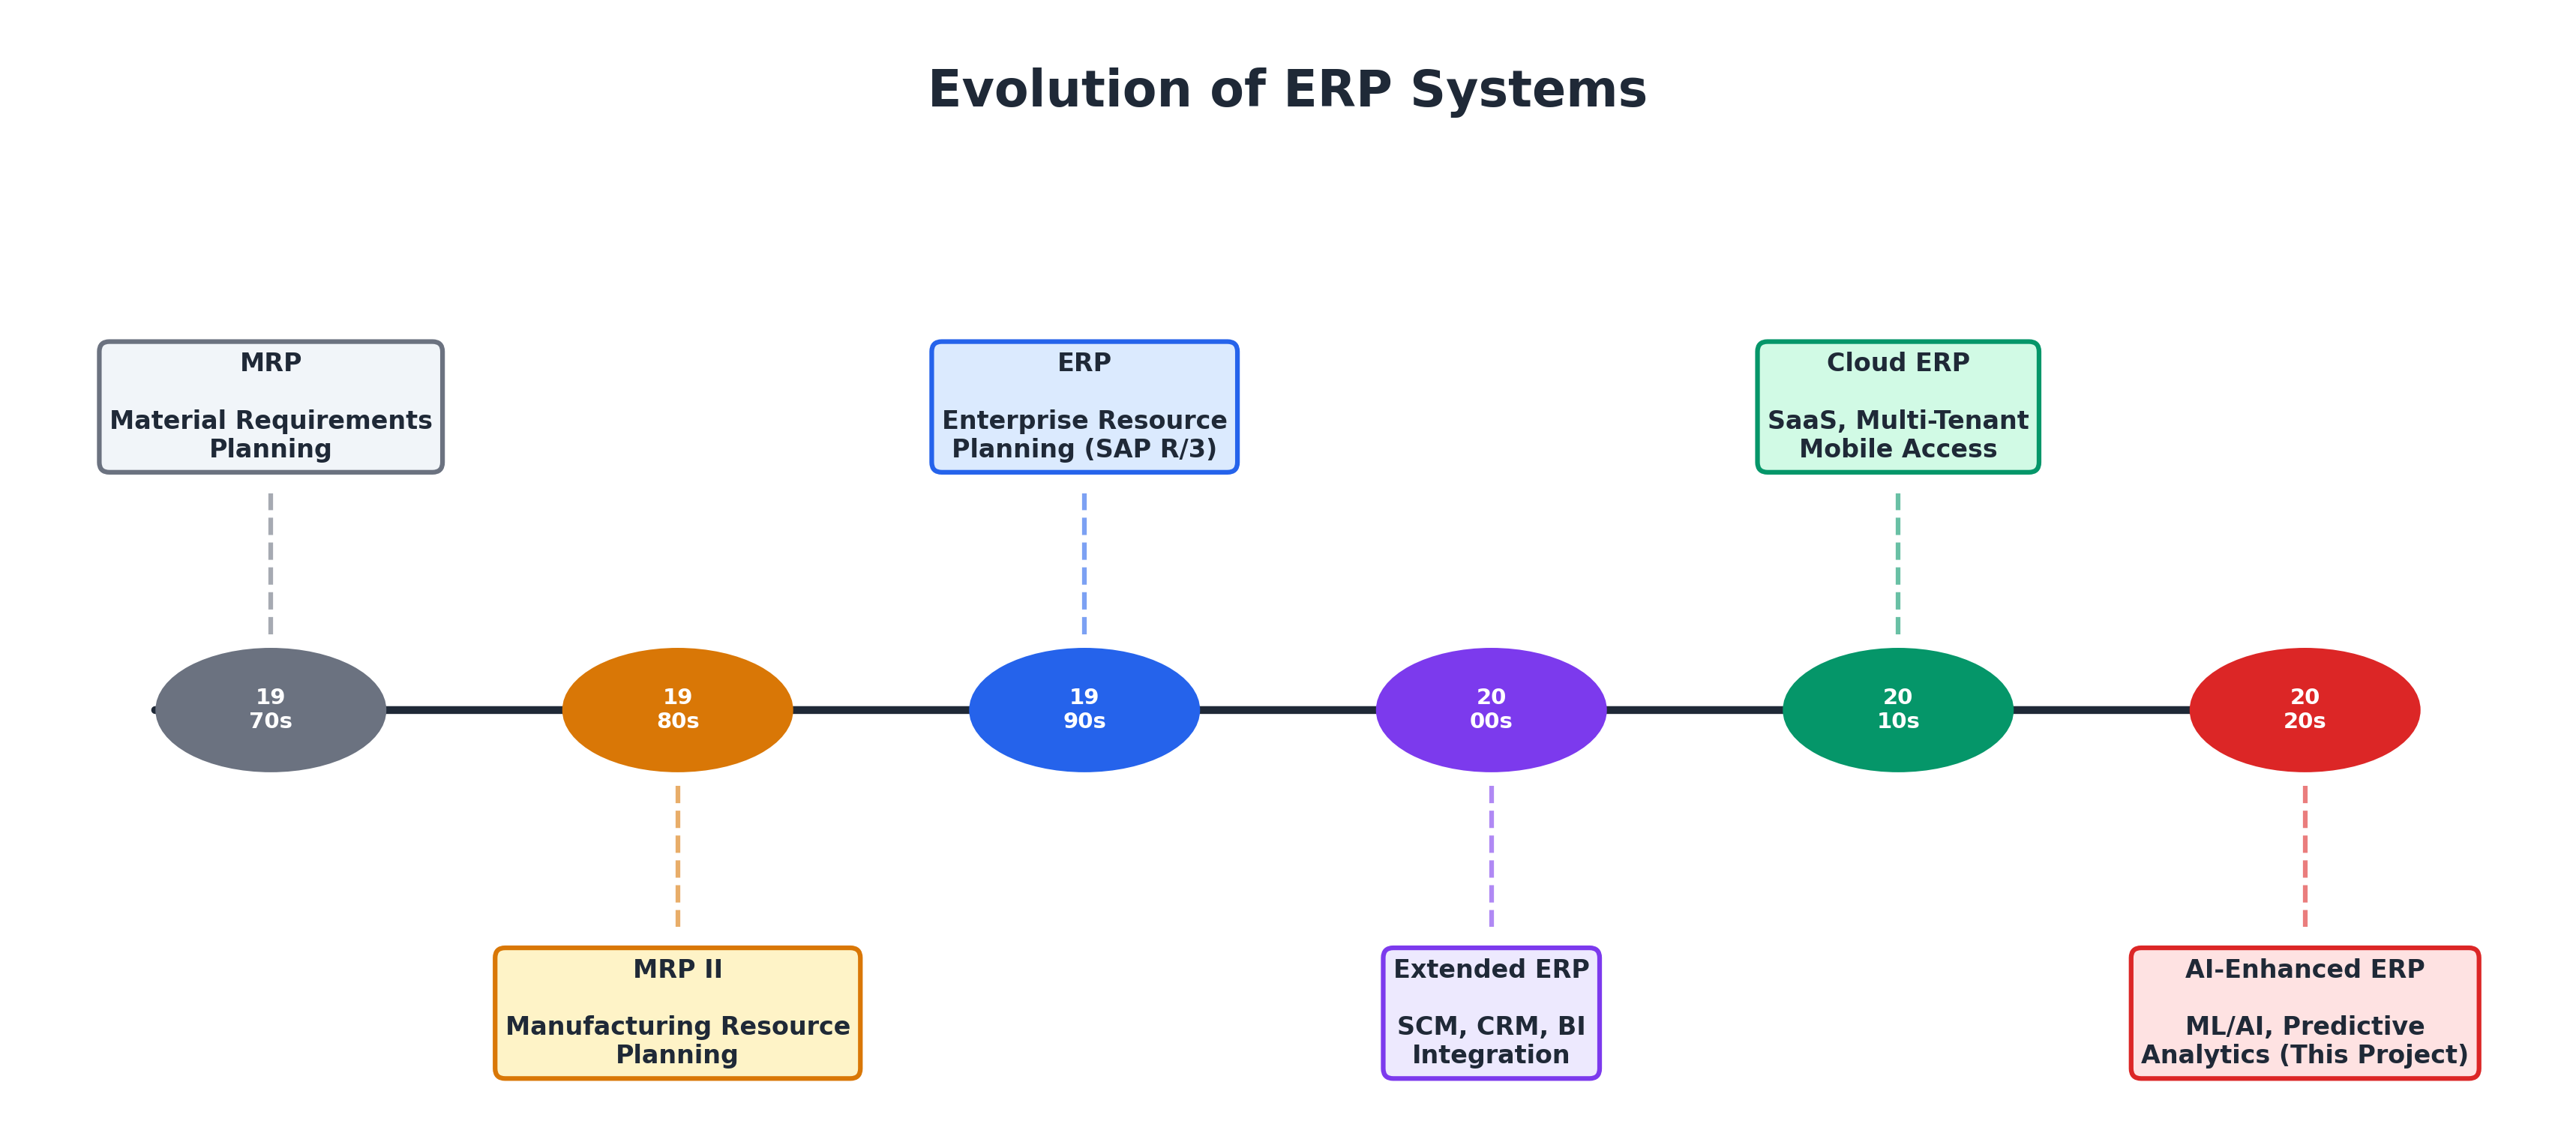
\includegraphics[width=0.95\textwidth]{figures/erp_evolution_timeline.png}
    \caption{Evolution of ERP systems from MRP (1970s) to Cloud AI-ERP (2020s)}
    \label{fig:erp_evolution}
\end{figure}

\subsection{ERP Architecture Models}

Modern ERP systems are typically deployed using one of three architectural models:

\begin{itemize}
  \item \textbf{Monolithic Architecture:} All modules are packaged as a single deployable unit sharing one database. Traditional SAP R/3 and Oracle E-Business Suite follow this model. While simple to deploy, monolithic architectures are difficult to scale and customize \citep{bezemer2010multi}.

  \item \textbf{Service-Oriented Architecture (SOA):} Business functions are decomposed into loosely coupled services that communicate via standardized protocols. Modern SAP S/4HANA adopts elements of SOA to enable extensibility \citep{krafzig2005enterprise}.

  \item \textbf{Microservices Architecture:} An evolution of SOA where each service is independently deployable and scalable. While offering maximum flexibility, this model introduces operational complexity that makes it less suitable for SME-focused projects \citep{newman2015building}.
\end{itemize}

This project adopts a \textbf{modular monolith} architecture---a single Django application with clearly separated modules (apps) that share a common codebase but maintain logical boundaries. This balances simplicity with maintainability and is well-suited for the project scope.

\subsection{ERP Adoption in SMEs}

Research by \citet{almajali2016antecedents} identifies organizational factors (top management support, organizational readiness), technological factors (system complexity, compatibility), and environmental factors (competitive pressure, vendor support) as determinants of ERP adoption success in Jordanian SMEs. Their findings highlight that \textit{perceived cost} and \textit{organizational readiness} are the strongest predictors of adoption intent.

A study by \citet{panorama2023} found that among organizations implementing ERP, 50\% reported exceeding their initial budget, and the average implementation timeline for SMEs was 14.3 months. These statistics underscore the need for lightweight, rapid-deployment ERP solutions---a gap this project addresses through its Django-based architecture and Sprint development methodology.

\subsection{Open-Source ERP Systems}

Several open-source ERP platforms have emerged as alternatives to commercial solutions:

\begin{table}[H]
\centering
\caption{Comparison of major open-source ERP systems}
\label{tab:erp_comparison}
\begin{tabularx}{\textwidth}{l X X X X}
\toprule
\textbf{Feature} & \textbf{Odoo CE} & \textbf{ERPNext} & \textbf{Dolibarr} & \textbf{This Project} \\
\midrule
Language & Python & Python/JS & PHP & Python (Django) \\
Database & PostgreSQL & MariaDB & MySQL/PgSQL & PostgreSQL \\
Multi-Tenant & Limited & No & No & \textbf{Yes (DB-per-tenant)} \\
Arabic Support & Partial & Partial & Minimal & \textbf{Full (dual fields)} \\
Integrated ML/AI & No & No & No & \textbf{8 ML models} \\
REST API & Yes & Yes & Limited & Yes (DRF) \\
WMS & Enterprise only & Basic & No & \textbf{Full WMS} \\
POS & Enterprise only & Basic & No & \textbf{Yes} \\
License & LGPL v3 & GPL v3 & GPL v3 & -- \\
\bottomrule
\end{tabularx}
\end{table}

As Table~\ref{tab:erp_comparison} illustrates, none of the existing open-source ERP systems combine native multi-tenant isolation, comprehensive Arabic support, and integrated machine learning capabilities---the three distinguishing features of this project.


\section{Multi-Tenant Software Architecture}
\label{sec:multi_tenant}

\subsection{Definition and Models}

Multi-tenancy is a software architecture principle in which a single instance of a software application serves multiple customers (tenants), each of whom perceives the application as if it were running exclusively for them \citep{bezemer2010multi}. Three principal models of multi-tenancy exist:

\begin{enumerate}[label=\arabic*.]
  \item \textbf{Shared Database, Shared Schema:} All tenants share the same database and tables, with a \texttt{tenant\_id} column used to filter data. This is the most resource-efficient model but offers the weakest data isolation and complicates compliance with data sovereignty regulations \citep{chong2006multi}.

  \item \textbf{Shared Database, Separate Schema:} Each tenant has its own database schema (namespace) within a shared database instance. This provides moderate isolation with lower overhead than full database separation. PostgreSQL's native schema support makes this model practical \citep{bezemer2010multi}.

  \item \textbf{Separate Database (Database-per-Tenant):} Each tenant is assigned a dedicated database instance. This model provides the strongest isolation---tenant data is physically separated, simplifying backup, migration, and regulatory compliance---at the cost of higher resource consumption \citep{bezemer2010multi}.
\end{enumerate}

\begin{figure}[H]
    \centering
    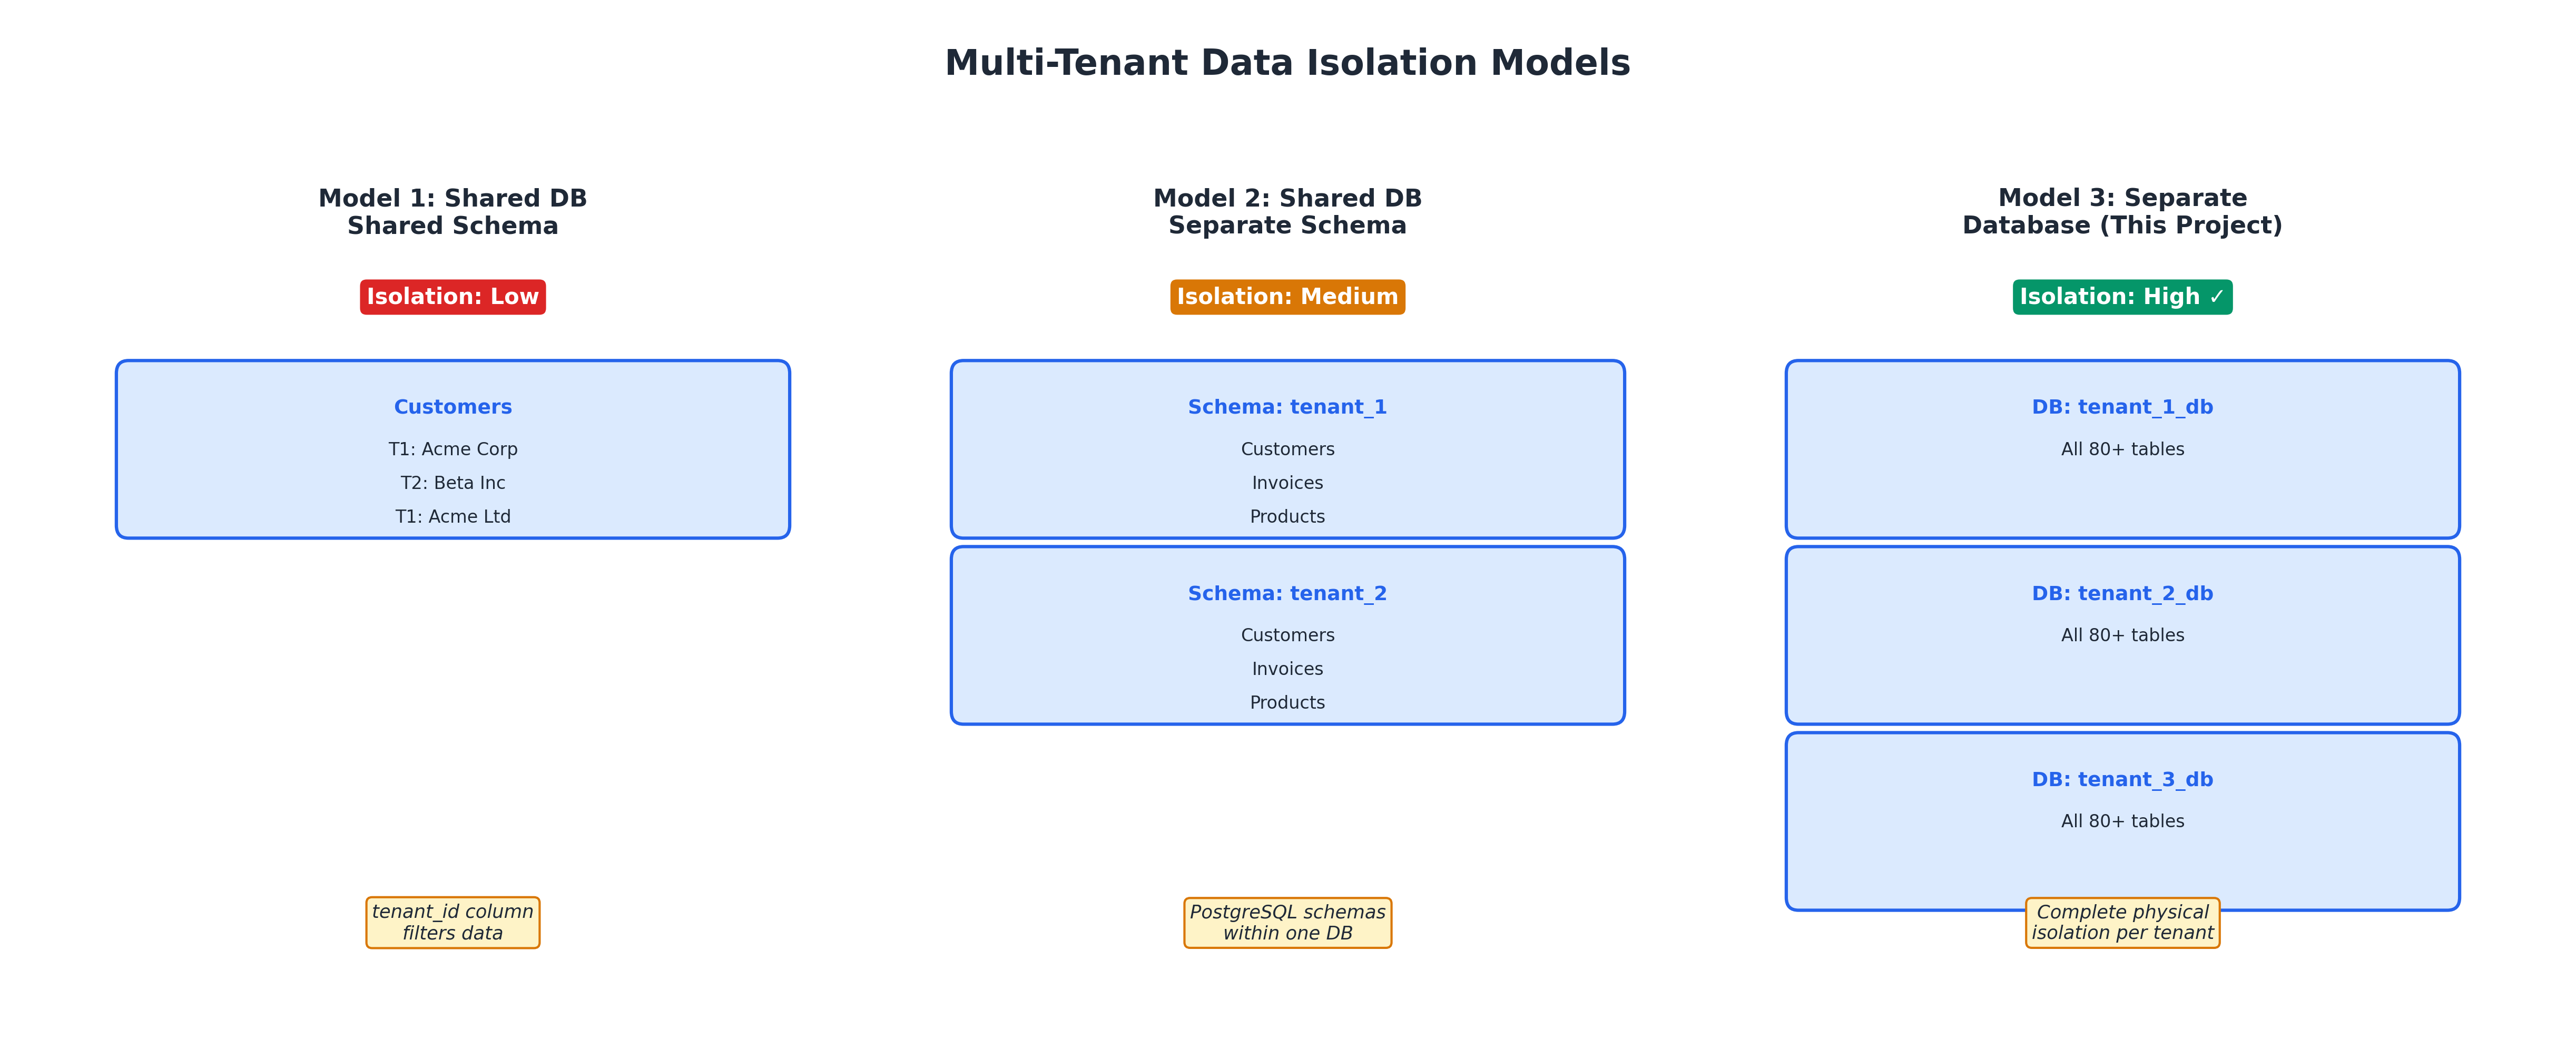
\includegraphics[width=0.95\textwidth]{figures/multi_tenancy_models.png}
    \caption{Three levels of multi-tenant data isolation}
    \label{fig:multi_tenancy_models}
\end{figure}

This project implements the \textbf{database-per-tenant} model, which provides the highest level of data isolation. Each tenant organization receives a dedicated PostgreSQL database that is dynamically provisioned via Docker containers or remote server connections. Django's database routing mechanism (\texttt{DATABASE\_ROUTERS}) is used to direct queries to the appropriate tenant database based on the authenticated user's session context.

\subsection{Multi-Tenancy in Django}

Django's built-in support for multiple databases, combined with custom database routers, makes it well-suited for implementing multi-tenant architectures. The key components in this project's implementation are:

\begin{itemize}
  \item \texttt{TenantDatabase} model: Stores connection parameters for each tenant's PostgreSQL database.
  \item \texttt{DatabaseAssignment} model: Maps users to tenant databases with role-based permissions.
  \item \texttt{add\_tenant\_database()}: Dynamically registers tenant database configurations in Django's \texttt{DATABASES} setting at runtime.
  \item \texttt{TenantDatabaseContext}: A context manager that sets the active database alias for the current thread, ensuring all ORM queries route to the correct tenant database.
  \item Custom middleware: Resolves the authenticated user's tenant database on each request and activates the appropriate database context.
\end{itemize}


\section{Machine Learning in Enterprise Systems}
\label{sec:ml_enterprise}

\subsection{Overview of ML in Business Applications}

The application of machine learning to business processes has accelerated significantly with the availability of large transactional datasets, affordable computing power, and mature ML frameworks. \citet{davenport2018ai} identify three levels of AI integration in business systems:

\begin{enumerate}[label=\arabic*.]
  \item \textbf{Process Automation:} Using ML for routine tasks such as document classification, data entry validation, and alert generation.
  \item \textbf{Cognitive Insight:} Applying ML algorithms to detect patterns in large datasets---such as customer segmentation, fraud detection, and demand forecasting---that would be impractical for human analysts.
  \item \textbf{Cognitive Engagement:} Deploying conversational AI and recommendation systems that interact directly with users, such as chatbots and personalized marketing engines.
\end{enumerate}

This project primarily operates at the \textbf{Cognitive Insight} level, embedding ML models that analyze transactional data and surface actionable insights to business users through the AI Insight Engine.

\subsection{Lead Scoring with Logistic Regression}

Lead scoring is the process of assigning a numerical value to each sales lead to predict the likelihood of conversion. While complex ensembles like gradient boosting are popular, simpler linear models such as Logistic Regression often provide highly robust, naturally interpretable baselines for CRM data where engagement patterns (activity counts) share direct linear relationships with conversion likelihood.

In this project, the Lead Scoring model uses 14 engineered features including estimated deal value, log-transformed value, activity count, activity-type breakdowns (calls, emails, meetings), engagement velocity (activities per day), lead source with target-encoded conversion rates, and customer contact completeness. Operational integrity is maintained by excluding proxy variables that would artificially inflate accuracy (such as time-since-creation for closed leads). The Logistic Regression model is trained on historical won/lost leads, scales features automatically, and outputs a conversion probability between 0 and 1, achieving a strong, realistic AUC-ROC of 0.9448.

\subsection{Payment Risk Prediction with Gradient Boosting}

Predicting whether an invoice will be paid late is a critical capability for accounts receivable management. \citet{chen2016xgboost} demonstrate that gradient boosted decision trees consistently outperform other classifiers on structured/tabular data tasks, making them ideal for invoice-level payment risk prediction.

The project's Late Payment Predictor uses 18 engineered features, including invoice amount, days to due date, customer historical payment delay, customer type, payment-term bucket, line-item count, and weekday indicators. Leave-one-out temporal statistics are used to prevent data leakage---a common pitfall identified by \citet{provost2013data} in churn and payment prediction models. During model optimisation, a \textit{balance\_ratio} feature (outstanding balance divided by total amount) was identified as a source of data leakage---since fully paid invoices inherently have a zero balance---and was removed, yielding an honest AUC-ROC of 0.6358 that reflects the genuine predictive signal in the feature set.

\subsection{Employee Attrition Prediction with Random Forest}

Employee turnover is costly, with the Society for Human Resource Management estimating replacement costs at 50--200\% of annual salary \citep{shrm2022}. \citet{breiman2001random} introduced Random Forest---an ensemble of decision trees trained on bootstrap samples---which has become a standard approach for employee attrition prediction due to its robustness to noisy features and native feature importance ranking.

This project's Attrition Predictor uses 13 operational features including tenure, salary relative to department average, leave frequency, attendance rate, overtime hours, and derived signals such as average gross salary, compensation ratio versus department average, and absence rate. Real-world predictive constraints are strictly enforced by stripping out "proxy" targets such as the raw count of historical payslips. Class imbalance (typically fewer departures than retentions) is addressed using the \texttt{class\_weight='balanced'} parameter, and the Random Forest is configured with 500 estimators and a maximum depth of 10, achieving a robust and strictly validated AUC-ROC of 0.9761 on the evaluation dataset.

\subsection{Anomaly Detection with Isolation Forest}

\citet{liu2008isolation} proposed the Isolation Forest algorithm based on the principle that anomalies are ``few and different''---they require fewer random partitions to isolate than normal observations. This makes Isolation Forest computationally efficient and effective for unsupervised anomaly detection in expense claim analysis, where labeled fraud data is typically unavailable.

The project's Expense Anomaly Detector applies Isolation Forest with a dynamically calibrated \texttt{contamination} parameter---computed from the interquartile range (IQR) of the training data and clamped between 0.01 and 0.15---to 11 engineered features including expense amount, category-level z-scores, employee-level z-scores, weekend submission flag, amount percentile rank, day of week, and month.

\subsection{Time-Series Forecasting with Prophet}

Facebook Prophet, introduced by \citet{taylor2018forecasting}, is an additive regression model designed for business time-series data with strong seasonal patterns and missing data points. Prophet decomposes the forecast into trend, seasonality (weekly, yearly, custom), and holiday components using a Bayesian framework.

The project uses Prophet for per-product demand forecasting, with custom monthly seasonality ($fourier\_order = 3$) and calibrated changepoint detection ($changepoint\_prior\_scale = 0.15$). Model accuracy is evaluated using Prophet's built-in cross-validation framework, achieving an average accuracy of approximately 0.72 across 80 product-warehouse combinations.

\subsection{Statistical Process Control for KPI Monitoring}

Z-score-based anomaly detection is a classical statistical quality control technique introduced by \citet{shewhart1931economic} and widely used in manufacturing as Shewhart control charts. When applied to business KPIs, the method flags values that deviate more than a specified number of standard deviations from the historical mean.

The project's KPI Anomaly Detector monitors five daily metrics (revenue, expenses, new leads, overdue invoices, inventory movements) against 90-day rolling baselines, generating WARNING alerts for deviations exceeding $2\sigma$ and CRITICAL alerts for deviations exceeding $3\sigma$.


\section{Explainable Artificial Intelligence (XAI)}
\label{sec:xai_literature}

\subsection{The Need for Explainability}

As ML models are deployed in high-stakes business decision systems, the demand for transparency has intensified from both regulatory and practical perspectives. The European Commission's High-Level Expert Group on AI identified \textit{transparency} and \textit{explicability} as two of seven key requirements for trustworthy AI \citep{eu2019ethics}. \citet{lipton2018mythos} distinguishes between \textit{transparency} (understanding the model's internal mechanics) and \textit{post-hoc interpretability} (explaining individual predictions after the fact), arguing that practical explanation needs vary by stakeholder: a data scientist may want feature interactions, while a business manager needs a ranked list of the top reasons behind a prediction.

\citet{doshi2017towards} formalise the notion that interpretability is not a monolithic property but depends on the explanation consumer, the task domain, and the evaluation criteria. In enterprise settings, explanations serve three purposes: (1)~\textit{trust calibration}---enabling users to decide when to accept or override a model's recommendation; (2)~\textit{model debugging}---helping developers diagnose errors, data leakage, or distribution shift; and (3)~\textit{regulatory compliance}---satisfying audit requirements for algorithmic decision-making.

\subsection{Taxonomy of XAI Methods}

\citet{arrieta2020explainable} provide a comprehensive taxonomy of XAI methods along several dimensions:

\begin{itemize}
  \item \textbf{Scope:} \textit{Global} methods explain the model's overall behaviour (e.g., which features matter most across all predictions), while \textit{local} methods explain individual predictions (e.g., why was this specific invoice flagged).

  \item \textbf{Stage:} \textit{Ante-hoc} methods build interpretability into the model itself (e.g., decision trees, linear regression), while \textit{post-hoc} methods explain an existing trained model without modifying it.

  \item \textbf{Model dependency:} \textit{Model-specific} methods exploit the internal structure of a particular algorithm (e.g., TreeExplainer for tree ensembles), while \textit{model-agnostic} methods treat the model as a black box and explain it by perturbing inputs and observing outputs.
\end{itemize}

\citet{guidotti2018survey} survey over 150 explanation methods and classify them into six families: feature attribution, rule extraction, prototype-based, counterfactual, attention-based, and example-based explanations. This project focuses on \textit{feature attribution} methods, which assign a numerical importance score to each input feature for a given prediction.

\subsection{SHAP: SHapley Additive exPlanations}

SHAP, introduced by \citet{lundberg2017unified}, unifies several existing explanation methods (LIME, DeepLIFT, Layer-wise Relevance Propagation) under the framework of \textit{Shapley values} from cooperative game theory \citep{shapley1953value}. The key insight is that explaining a prediction is analogous to dividing the ``payout'' (the prediction's deviation from the baseline) among the ``players'' (input features) in a fair manner.

The Shapley value $\phi_i$ of feature $i$ is defined as:

\begin{equation}
\phi_i = \sum_{S \subseteq N \setminus \{i\}} \frac{|S|! \; (|N| - |S| - 1)!}{|N|!} \left[ f(S \cup \{i\}) - f(S) \right]
\label{eq:shapley}
\end{equation}

\noindent where $N$ is the set of all features, $S$ is a subset excluding feature $i$, and $f(S)$ is the model's expected output given only the features in $S$. The Shapley value represents the average marginal contribution of feature $i$ across all possible feature orderings, satisfying four desirable properties \citep{lundberg2017unified}:

\begin{enumerate}[label=\arabic*.]
  \item \textbf{Local accuracy (efficiency):} $\sum_{i=1}^{|N|} \phi_i = f(x) - \mathbb{E}[f(X)]$ --- the attributions sum to the difference between the prediction and the baseline.
  \item \textbf{Missingness:} If a feature is absent from the model, its attribution is zero.
  \item \textbf{Consistency:} If a feature's marginal contribution increases in a new model, its attribution does not decrease.
  \item \textbf{Symmetry:} Features with equal contributions receive equal attributions.
\end{enumerate}

For tree-based models, \citet{lundberg2020local} developed \textbf{TreeExplainer}, an algorithm that computes exact Shapley values in $O(TLD^2)$ time (where $T$ is the number of trees, $L$ is the maximum number of leaves, and $D$ is the maximum depth), making it practical for production use with Gradient Boosting and Random Forest models containing hundreds of trees.

\subsection{LIME: Local Interpretable Model-agnostic Explanations}

LIME, introduced by \citet{ribeiro2016why}, explains individual predictions by approximating the model locally with an interpretable surrogate model. The procedure is:

\begin{enumerate}[label=\arabic*.]
  \item \textbf{Perturb:} Generate synthetic samples near the instance to be explained by randomly toggling features on/off.
  \item \textbf{Predict:} Obtain the original model's prediction for each perturbed sample.
  \item \textbf{Weight:} Assign higher weights to perturbed samples closer to the original instance (using an exponential kernel).
  \item \textbf{Fit:} Train a weighted linear regression on the perturbed dataset to obtain feature coefficients.
  \item \textbf{Explain:} The linear coefficients represent each feature's local contribution to the prediction.
\end{enumerate}

Formally, LIME seeks the explanation $\xi$ that minimises:

\begin{equation}
\xi(x) = \argmin_{g \in G} \; \mathcal{L}(f, g, \pi_x) + \Omega(g)
\label{eq:lime}
\end{equation}

\noindent where $f$ is the original model, $g$ is the interpretable surrogate, $\pi_x$ is the proximity kernel centred on instance $x$, $\mathcal{L}$ is the fidelity loss (how well $g$ approximates $f$ locally), and $\Omega(g)$ is a complexity penalty (e.g., limiting the number of non-zero coefficients).

LIME is model-agnostic---it can explain any classifier or regressor---but its explanations are \textit{approximate} and can vary across runs due to the stochastic perturbation process. \citet{slack2020fooling} demonstrate that LIME explanations can be manipulated by adversarially designed models, highlighting the importance of using multiple explanation methods (e.g., SHAP + LIME) for cross-validation.

\subsection{SHAP vs.\ LIME: Complementary Strengths}

Table~\ref{tab:shap_vs_lime} summarises the key differences between SHAP and LIME:

\begin{table}[H]
\centering
\caption{Comparison of SHAP and LIME explanation methods}
\label{tab:shap_vs_lime}
\begin{tabularx}{\textwidth}{l >{\raggedright\arraybackslash}X >{\raggedright\arraybackslash}X}
\toprule
\textbf{Property} & \textbf{SHAP (TreeExplainer)} & \textbf{LIME (TabularExplainer)} \\
\midrule
Theoretical basis & Shapley values (game theory) & Locally-faithful linear surrogate \\
Guarantees & Exact local accuracy, consistency, symmetry & Approximate local fidelity \\
Model dependency & Tree-specific (exact); kernel (approx.) & Model-agnostic \\
Determinism & Deterministic for tree models & Stochastic (random perturbations) \\
Global explanations & Yes (mean $|\text{SHAP}|$ aggregation) & No (instance-level only) \\
Computation cost & $O(TLD^2)$ per instance & $O(n_{\text{perturb}} \cdot T_{\text{predict}})$ \\
Additivity & $\sum \phi_i = f(x) - E[f]$ & No additivity guarantee \\
\bottomrule
\end{tabularx}
\end{table}

Using both methods provides \textit{explanation triangulation}: when SHAP and LIME agree on the top contributing features, confidence in the explanation is high; when they diverge, it signals that the model may behave non-linearly in the local neighbourhood, warranting closer inspection \citep{molnar2022interpretable}.

\subsection{XAI as a Model Validation Tool}

Beyond user-facing transparency, XAI methods have proven effective for \textit{model debugging} and \textit{data-quality validation}. \citet{lundberg2020local} demonstrate that aggregating SHAP values across a dataset reveals unexpected feature dominance---a telltale sign of data leakage, where a feature carries information that would not be available at prediction time in production.

For example, if a payment-prediction model assigns 60\%+ of its total SHAP importance to a single engineered feature, this disproportionate reliance suggests that the feature may encode the target variable (data leakage) rather than capturing a genuine predictive pattern. Standard metrics such as AUC-ROC report high performance regardless, because the leaked feature genuinely correlates with the target---but the model would fail catastrophically in deployment where the leaked feature's value is not available \citep{molnar2022interpretable}.

This use of XAI for model validation is a central theme of this project: the evaluation in Chapter~6 demonstrates that SHAP analysis surfaced data-leakage issues in 2 of 3 ML models that reported excellent AUC-ROC scores.


\section{Related Work}
\label{sec:related_work}

\subsection{AI-Enhanced ERP Systems}

\citet{lee2020erp} survey the integration of AI technologies into ERP systems and identify three implementation strategies: (1)~embedded AI within the ERP platform itself, (2)~AI as an external service integrated via APIs, and (3)~AI as a middleware layer between the ERP and a BI platform. They conclude that the embedded approach provides the tightest integration and lowest latency but requires the deepest technical expertise. This project follows the embedded approach.

SAP introduced ``SAP Business AI'' in 2023, incorporating predictive analytics and natural language processing into S/4HANA Cloud. However, these capabilities are available only in the Enterprise tier, which carries substantial licensing costs. Oracle Fusion Cloud ERP similarly offers ML-driven anomaly detection and forecasting features in its premium offerings. No open-source ERP system currently provides comparable embedded ML capabilities, let alone post-hoc XAI explanations for its predictions.

\subsection{XAI in Business Decision Systems}

Several studies have applied SHAP and LIME to business-domain ML models, but \textit{none} embed these explanations within an operational ERP system:

\begin{itemize}
  \item \citet{lundberg2020local} apply TreeSHAP to medical risk prediction models and demonstrate that global SHAP importance plots can reveal data-quality issues. Their work establishes the ``XAI as debugging'' paradigm that this project extends to ERP-domain models.

  \item \citet{molnar2022interpretable} provides a comprehensive practitioner's guide to SHAP, LIME, and other IML methods, with case studies in credit scoring and customer churn prediction. The guide recommends using multiple explanation methods for cross-validation---an approach adopted in this project.

  \item \citet{slack2020fooling} demonstrate that LIME explanations can be manipulated by adversarially designed models, underscoring the need for SHAP's theoretical guarantees as a complementary check. This motivates the dual SHAP+LIME approach in this project.

  \item \citet{rudin2019stop} argues that for high-stakes decisions, inherently interpretable models should be preferred over post-hoc explanations of black boxes. While this position has merit, in the ERP context where complex models (like Random Forests and Gradient Boosting) often outperform simpler linear classifiers, post-hoc explanations offer a pragmatic middle ground.
\end{itemize}

\subsection{Multi-Tenant Django Applications}

The \texttt{django-tenants} library implements PostgreSQL schema-based multi-tenancy for Django, providing automatic schema routing via the \texttt{search\_path} mechanism. While this approach is well-tested, it does not support database-per-tenant isolation, which this project requires for maximum data separation. The \texttt{django-db-multitenant} library offers a middleware-based approach but is limited to schema-based or connection-string routing. This project implements a custom multi-tenant framework with dynamic database registration, Docker-based provisioning, and a user approval workflow---features not provided by existing libraries.

\subsection{ML for Demand Forecasting in Supply Chain}

\citet{fildes2022forecasting} provide a comprehensive review of ML approaches for retail demand forecasting, comparing classical time-series methods (ARIMA, Exponential Smoothing) with machine learning methods (Random Forest, Gradient Boosting, Neural Networks) and hybrid approaches. They find that Prophet performs competitively on datasets with strong seasonality and limited history, making it well-suited for SME inventory data where per-product histories may span only 6--12 months.


\section{Gap Analysis}
\label{sec:gap_analysis}

The literature review reveals the following gaps that this project addresses:

\begin{table}[H]
\centering
\caption{Literature gap analysis and project contributions}
\label{tab:gap_analysis}
\begin{tabularx}{\textwidth}{>{\raggedright\arraybackslash}X >{\raggedright\arraybackslash}X >{\raggedright\arraybackslash}X}
\toprule
\textbf{Gap Identified} & \textbf{Supporting Literature} & \textbf{Project Contribution} \\
\midrule
No open-source ERP with embedded ML & \citet{lee2020erp}; SAP/Oracle features are premium-only & 8 ML models embedded in a free, open-source ERP \\
\addlinespace
No XAI explanations in ERP ML models & \citet{arrieta2020explainable}; \citet{rudin2019stop}; commercial ERP AI provides no per-prediction justification & \textbf{Dual SHAP + LIME explanations} for 3 tree-based classifiers with waterfall, beeswarm, and force-plot visualisations \\
\addlinespace
ML metrics mask data-quality issues & \citet{lundberg2020local}; \citet{molnar2022interpretable}; AUC-ROC does not reveal feature leakage & \textbf{XAI as model validation}: SHAP exposed data leakage in 2/3 models \\
\addlinespace
Limited multi-tenant options in Django & django-tenants supports schema-only; django-db-multitenant lacks provisioning & Custom DB-per-tenant with Docker provisioning and role-based access \\
\addlinespace
Poor Arabic support in open-source ERP & \citet{alkraiji2020}; Odoo/ERPNext have partial translations & Dual-language fields (\texttt{name}/\texttt{name\_ar}) in 80+ models \\
\addlinespace
ML models disconnected from ERP workflow & Most ML-ERP integrations use external BI tools & Inline ML training, prediction logging, and AI Insight notifications \\
\addlinespace
Lack of cross-domain ML in single ERP & Studies focus on single domains (finance OR HR OR supply chain) & Models span CRM, Finance, HR, Inventory, and Operations \\
\bottomrule
\end{tabularx}
\end{table}

\section{Summary}
\label{sec:lit_summary}

This chapter reviewed the evolution and current state of ERP systems, multi-tenant software architectures, the application of machine learning in enterprise settings, and the theoretical foundations of Explainable AI---including SHAP's Shapley-value framework and LIME's locally-faithful surrogate approach. The review established that while commercial ERP vendors have begun incorporating AI capabilities, these features remain inaccessible to SMEs due to cost and complexity, and \textit{none} provide per-prediction explanations to business users. Open-source ERP alternatives lack both native multi-tenancy and integrated ML. Furthermore, the literature demonstrates that XAI methods can serve as model validation tools by surfacing data-quality issues that aggregate metrics fail to detect. This project bridges these gaps by combining a production-quality multi-tenant ERP with eight embedded ML models augmented by a dual SHAP+LIME explainability framework, delivered through an Agile Sprint development process that is detailed in the following chapter.


% ██████████████████████████████████████████████████████████████████
%
%  CHAPTER 3 — METHODOLOGY
%
% ██████████████████████████████████████████████████████████████████
\chapter{Methodology}
\label{ch:methodology}

\section{Introduction}
\label{sec:meth_intro}

This chapter presents the development methodology, system architecture, technology stack, data collection approach, and machine learning pipeline design adopted for this project. The Sprint (Agile) methodology was selected as the software development lifecycle (SDLC) model to accommodate the project's complexity, evolving requirements, and the iterative nature of ML model development.

\section{Development Methodology: Sprint (Agile)}
\label{sec:sprint_methodology}

\subsection{Overview of Sprint Methodology}

The Sprint methodology, as defined in the Scrum framework \citep{schwaber2020scrum}, organizes software development into fixed-length iterations called \textbf{Sprints}, typically lasting 1--4 weeks. Each Sprint follows a structured cycle: planning, development, testing, review, and retrospective. This iterative approach is particularly well-suited for projects with complex, multi-module architectures and evolving requirements---both characteristics of this ERP system.

\begin{figure}[H]
    \centering
    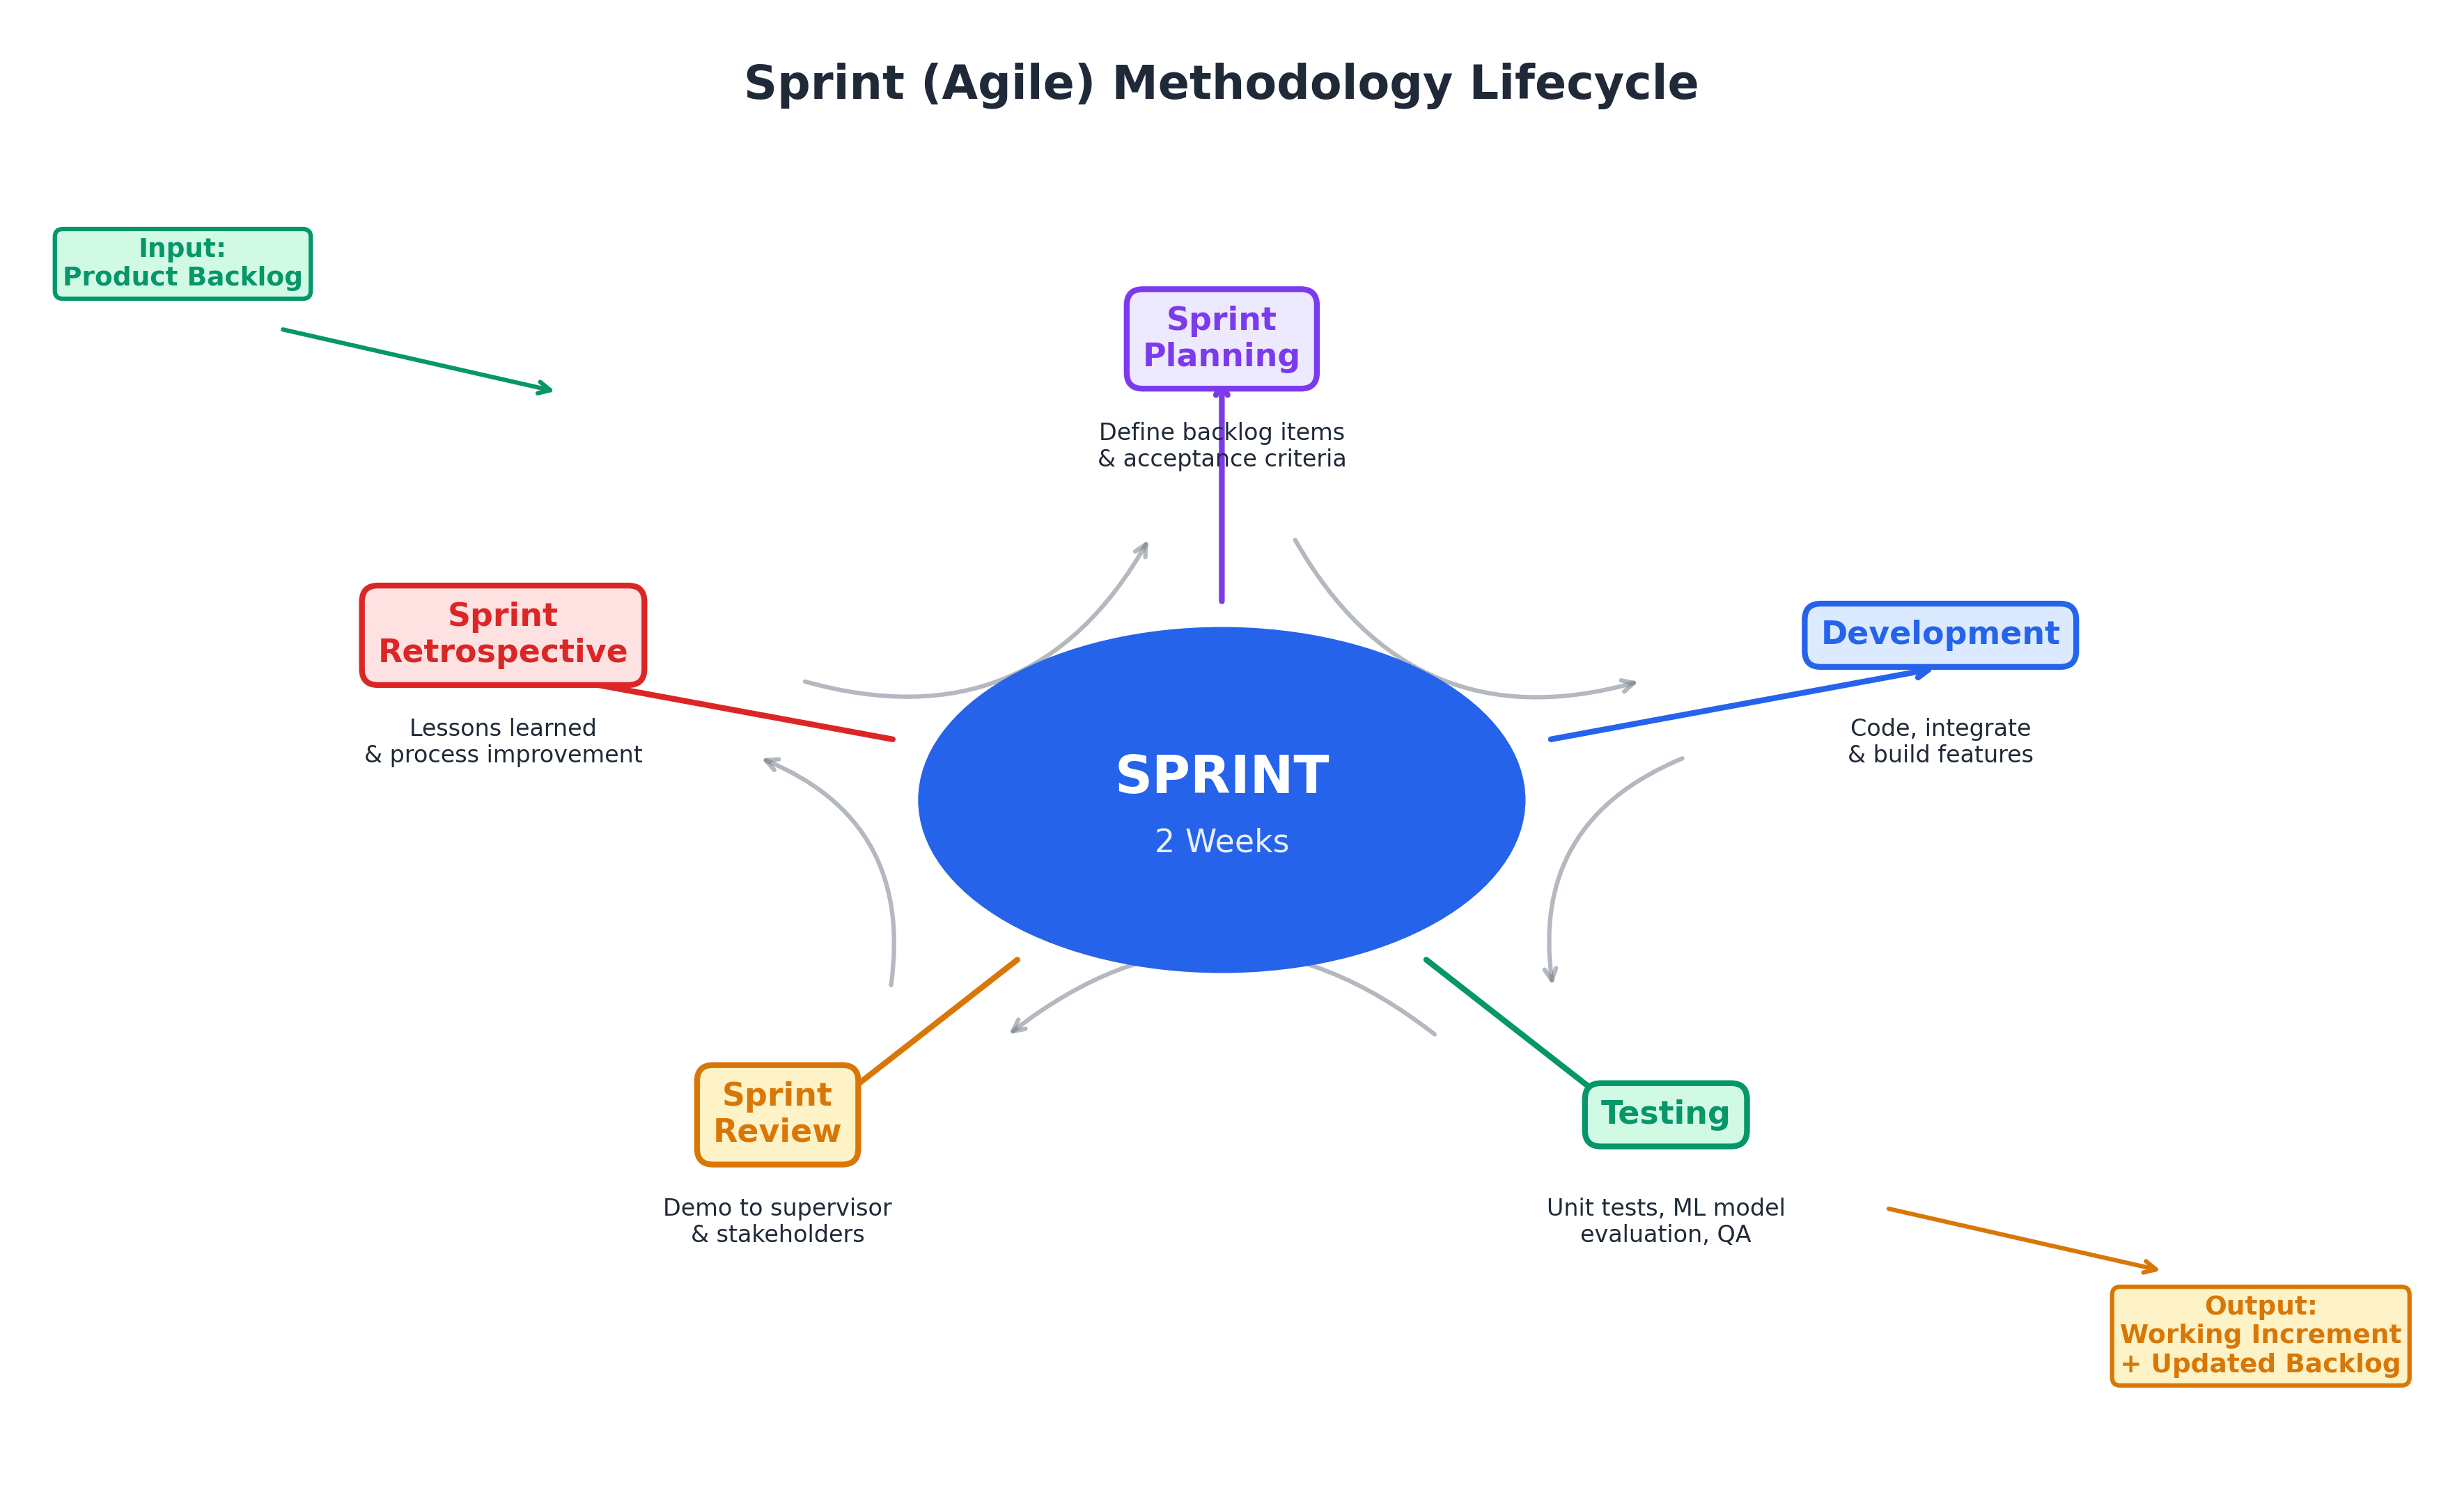
\includegraphics[width=0.85\textwidth]{figures/sprint_lifecycle.png}
    \caption{Sprint (Agile) methodology lifecycle}
    \label{fig:sprint_lifecycle}
\end{figure}

The key principles of the Sprint methodology applied to this project include:

\begin{itemize}
  \item \textbf{Iterative Delivery:} Each Sprint produces a working increment of the system, allowing stakeholders to review functional modules progressively rather than waiting for a final monolithic delivery.

  \item \textbf{Adaptive Planning:} Sprint planning sessions at the beginning of each iteration allow the team to reprioritize tasks based on feedback, discovered dependencies, and technical challenges.

  \item \textbf{Continuous Integration and Testing:} Code is tested at the end of each Sprint, including unit tests for ML model accuracy and integration tests for API endpoints.

  \item \textbf{Feedback-Driven Improvement:} Sprint retrospectives identify process improvements, while Sprint reviews validate that delivered features meet acceptance criteria.
\end{itemize}

\subsection{Sprint Plan for This Project}

The project was organized into \textbf{eight Sprints} over the development period. Table~\ref{tab:sprint_plan} summarizes the Sprint plan:

\begin{table}[H]
\centering
\caption{Sprint plan and deliverables}
\label{tab:sprint_plan}
\begin{tabularx}{\textwidth}{c c >{\raggedright\arraybackslash}X >{\raggedright\arraybackslash}X}
\toprule
\textbf{Sprint} & \textbf{Duration} & \textbf{Focus Area} & \textbf{Deliverables} \\
\midrule
1 & 2 weeks & Project Setup \& Multi-Tenant Architecture & Django project scaffold, TenantUser model, PostgresServer model, TenantDatabase model, database routing, user approval workflow \\
\addlinespace
2 & 2 weeks & Core ERP Modules (Finance \& HR) & Company, Currency, Department, Employee, Attendance, Payroll, Invoice, Payment, Expense, Chart of Accounts \\
\addlinespace
3 & 2 weeks & CRM, Supplier \& Procurement & Lead, LeadActivity, Campaign, Customer, Supplier, PurchaseOrder, SupplierInvoice, SupplierPayment \\
\addlinespace
4 & 2 weeks & Inventory/WMS \& POS & Warehouse, zones/bins, StockMovement, GoodsReceipt, StockTransfer, CycleCount, PickList, ShipmentNote, ReorderRule, POS terminal/session/order \\
\addlinespace
5 & 2 weeks & ML Model Development & AI model registry, 8 ML service modules, training pipeline, prediction logging, AI Insight engine \\
\addlinespace
6 & 2 weeks & Data Integration \& ML Tuning & Dataset import commands, synthetic data seeding, Prophet hyperparameter tuning, KPI calibration, model evaluation \\
\addlinespace
7 & 2 weeks & Testing, Documentation \& Deployment & Integration testing, API documentation, deployment configuration (Gunicorn + Docker), thesis writing \\
\addlinespace
8 & 2 weeks & Explainable AI Module & ExplainabilityService (SHAP TreeExplainer + LIME TabularExplainer), ExplanationResult model, XAI API endpoints, XAI web views and templates, global/instance explanation evaluations, data-leakage analysis \\
\bottomrule
\end{tabularx}
\end{table}

\begin{figure}[H]
    \centering
    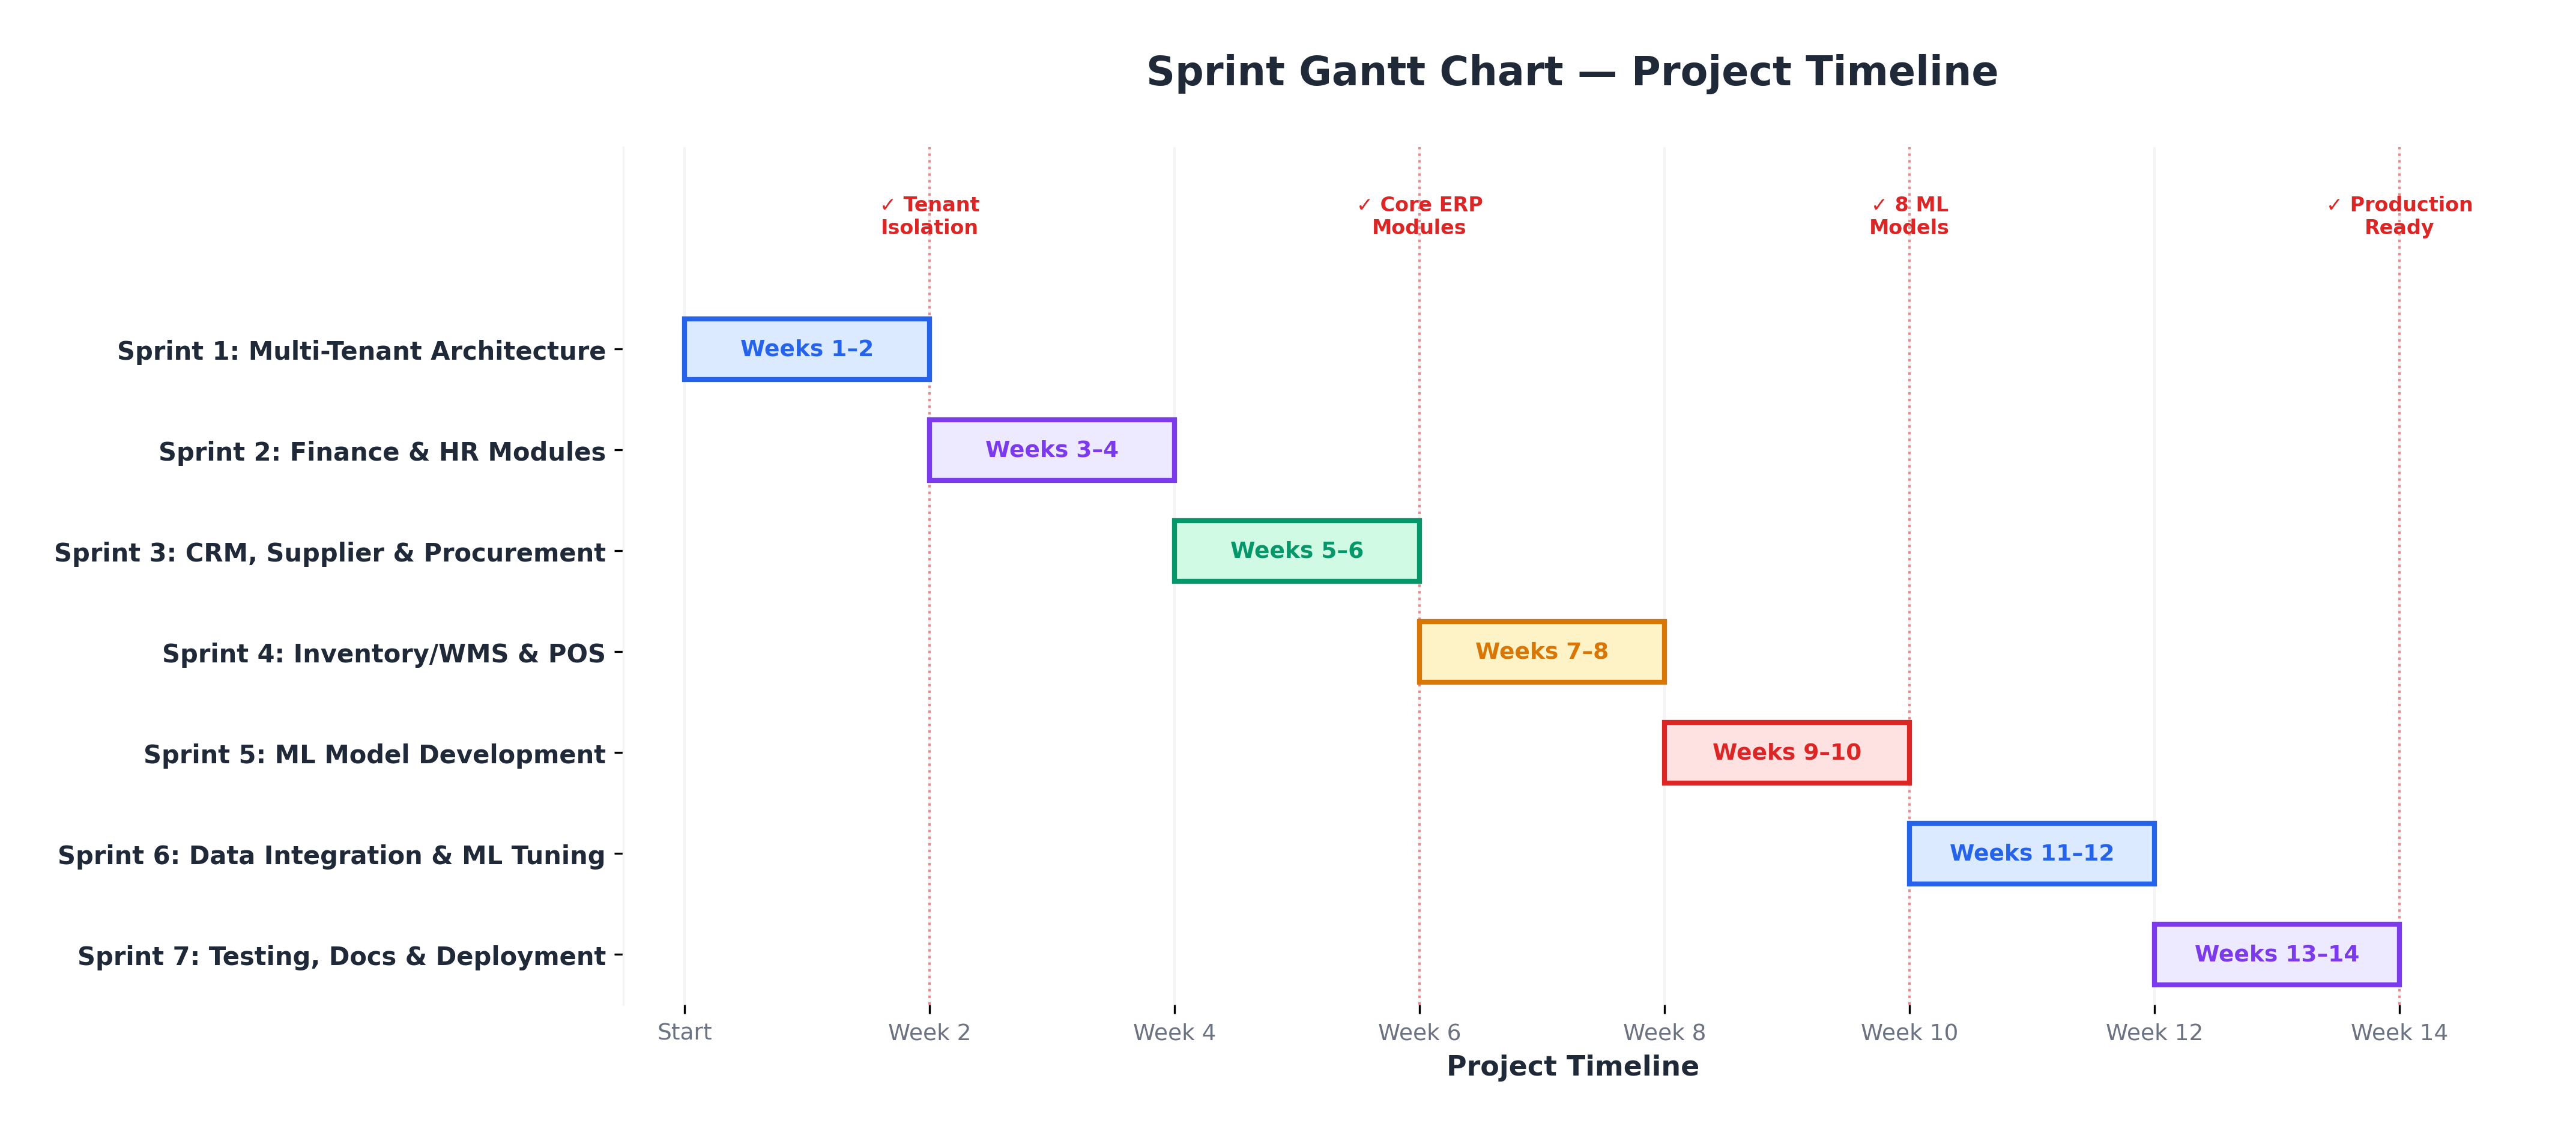
\includegraphics[width=0.95\textwidth]{figures/sprint_gantt_chart.png}
    \caption{Gantt chart showing Sprint timeline and dependencies}
    \label{fig:gantt_chart}
\end{figure}

\subsection{Sprint Roles}

Although this is an individual graduation project, the Sprint methodology roles were adapted as follows:

\begin{itemize}
  \item \textbf{Product Owner:} The project supervisor, who reviewed Sprint deliverables and provided feedback on priorities and acceptance criteria.
  \item \textbf{Scrum Master / Developer:} The student (Ahmed AMeen Hassan Alkuraimi), responsible for Sprint planning, development, testing, and retrospective documentation.
  \item \textbf{Stakeholders:} The academic committee and potential end users who provided domain feedback during the CRM, Finance, and HR module development.
\end{itemize}

\subsection{Justification for Sprint Methodology}

The Sprint methodology was chosen over alternative SDLC models for the following reasons:

\begin{table}[H]
\centering
\caption{SDLC model comparison and justification}
\label{tab:sdlc_comparison}
\begin{tabularx}{\textwidth}{l >{\raggedright\arraybackslash}X >{\raggedright\arraybackslash}X}
\toprule
\textbf{SDLC Model} & \textbf{Strengths} & \textbf{Limitation for This Project} \\
\midrule
Waterfall & Clear phases, thorough documentation & Does not accommodate changing requirements; ML models require iterative tuning \\
\addlinespace
V-Model & Strong testing emphasis & Sequential nature delays integration testing \\
\addlinespace
RAD & Rapid prototyping & Insufficient emphasis on architecture for a system with 80+ models \\
\addlinespace
\textbf{Sprint (Agile)} & Iterative delivery, accommodates ML experimentation, continuous feedback & Requires discipline in documentation (addressed through Sprint reviews) \\
\bottomrule
\end{tabularx}
\end{table}


\section{System Architecture}
\label{sec:architecture}

\subsection{High-Level Architecture}

The system follows a three-tier architecture: Presentation Layer (Django templates + REST API), Application Layer (Django views, services, and ML pipelines), and Data Layer (PostgreSQL databases with multi-tenant routing).

\begin{figure}[H]
    \centering
    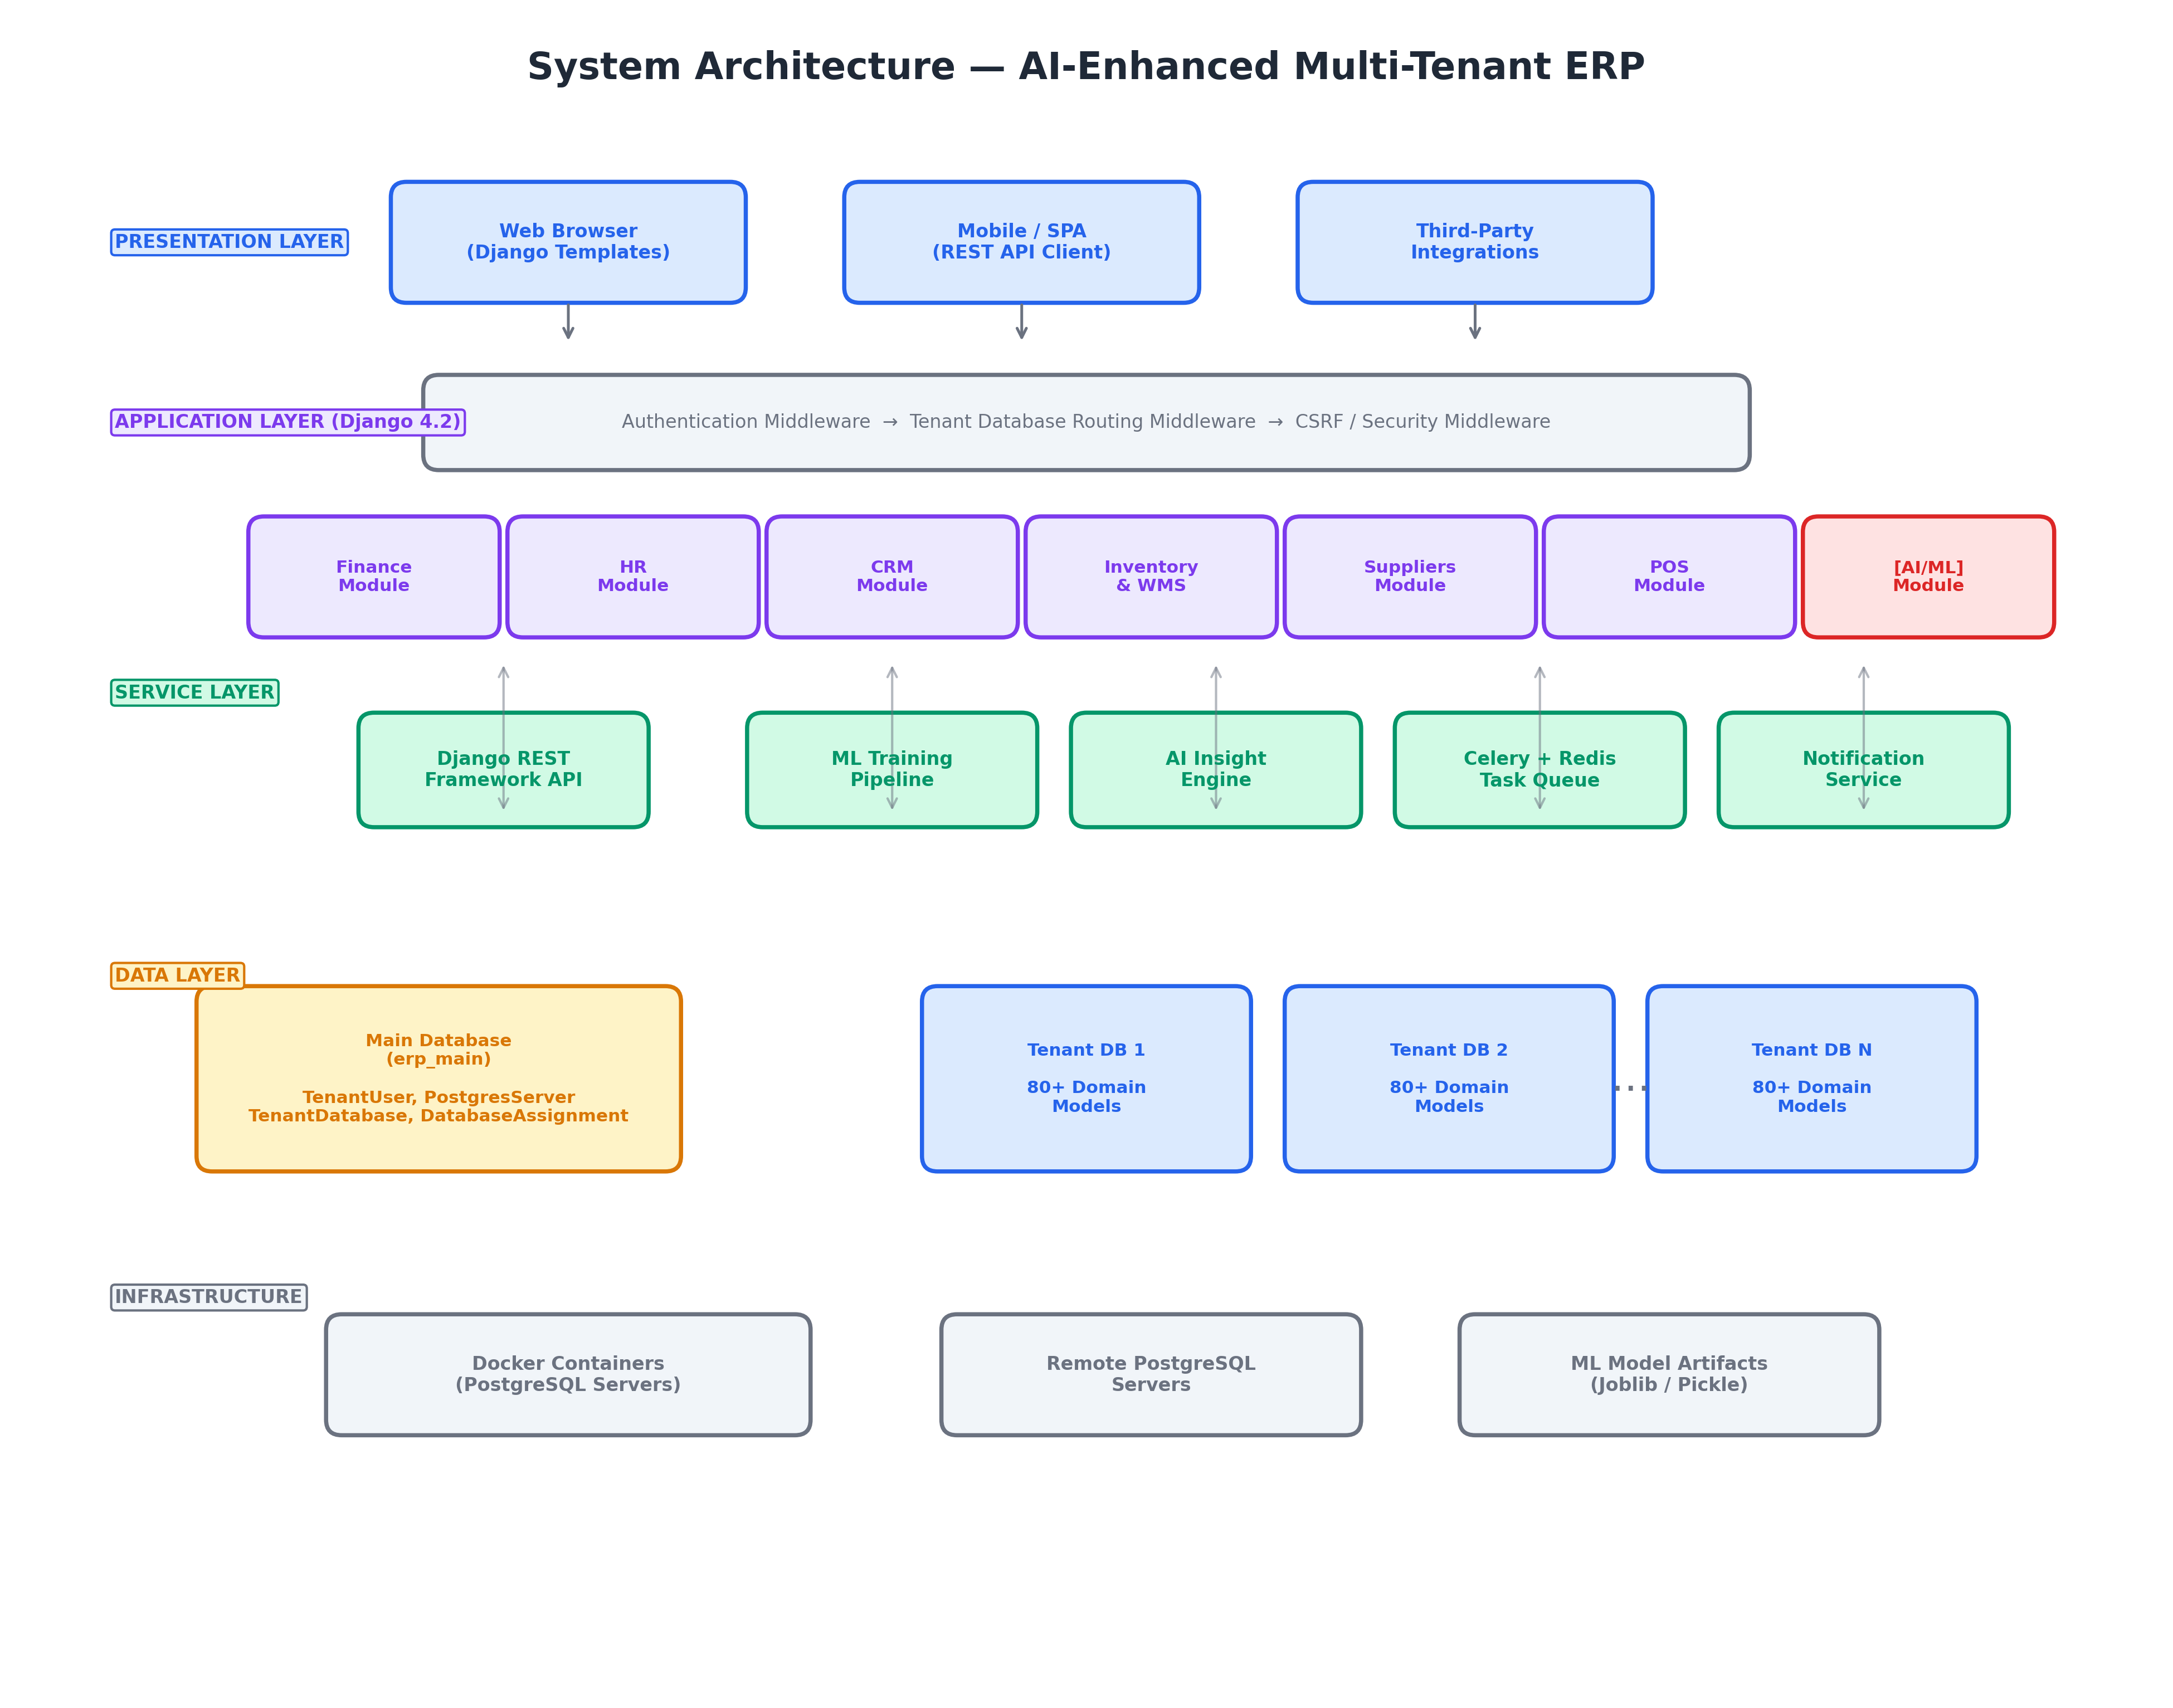
\includegraphics[width=0.95\textwidth]{figures/system_architecture.png}
    \caption{High-level system architecture showing the three-tier design with multi-tenant database routing}
    \label{fig:system_architecture}
\end{figure}

\subsection{Multi-Tenant Database Architecture}

The multi-tenant architecture is implemented using the database-per-tenant isolation model. The platform maintains a \textbf{main database} (\texttt{erp\_main}) that stores user accounts, server configurations, and tenant metadata. Each approved tenant organization receives a dedicated PostgreSQL database provisioned on a selected server (Docker container or remote server).

\begin{figure}[H]
    \centering
    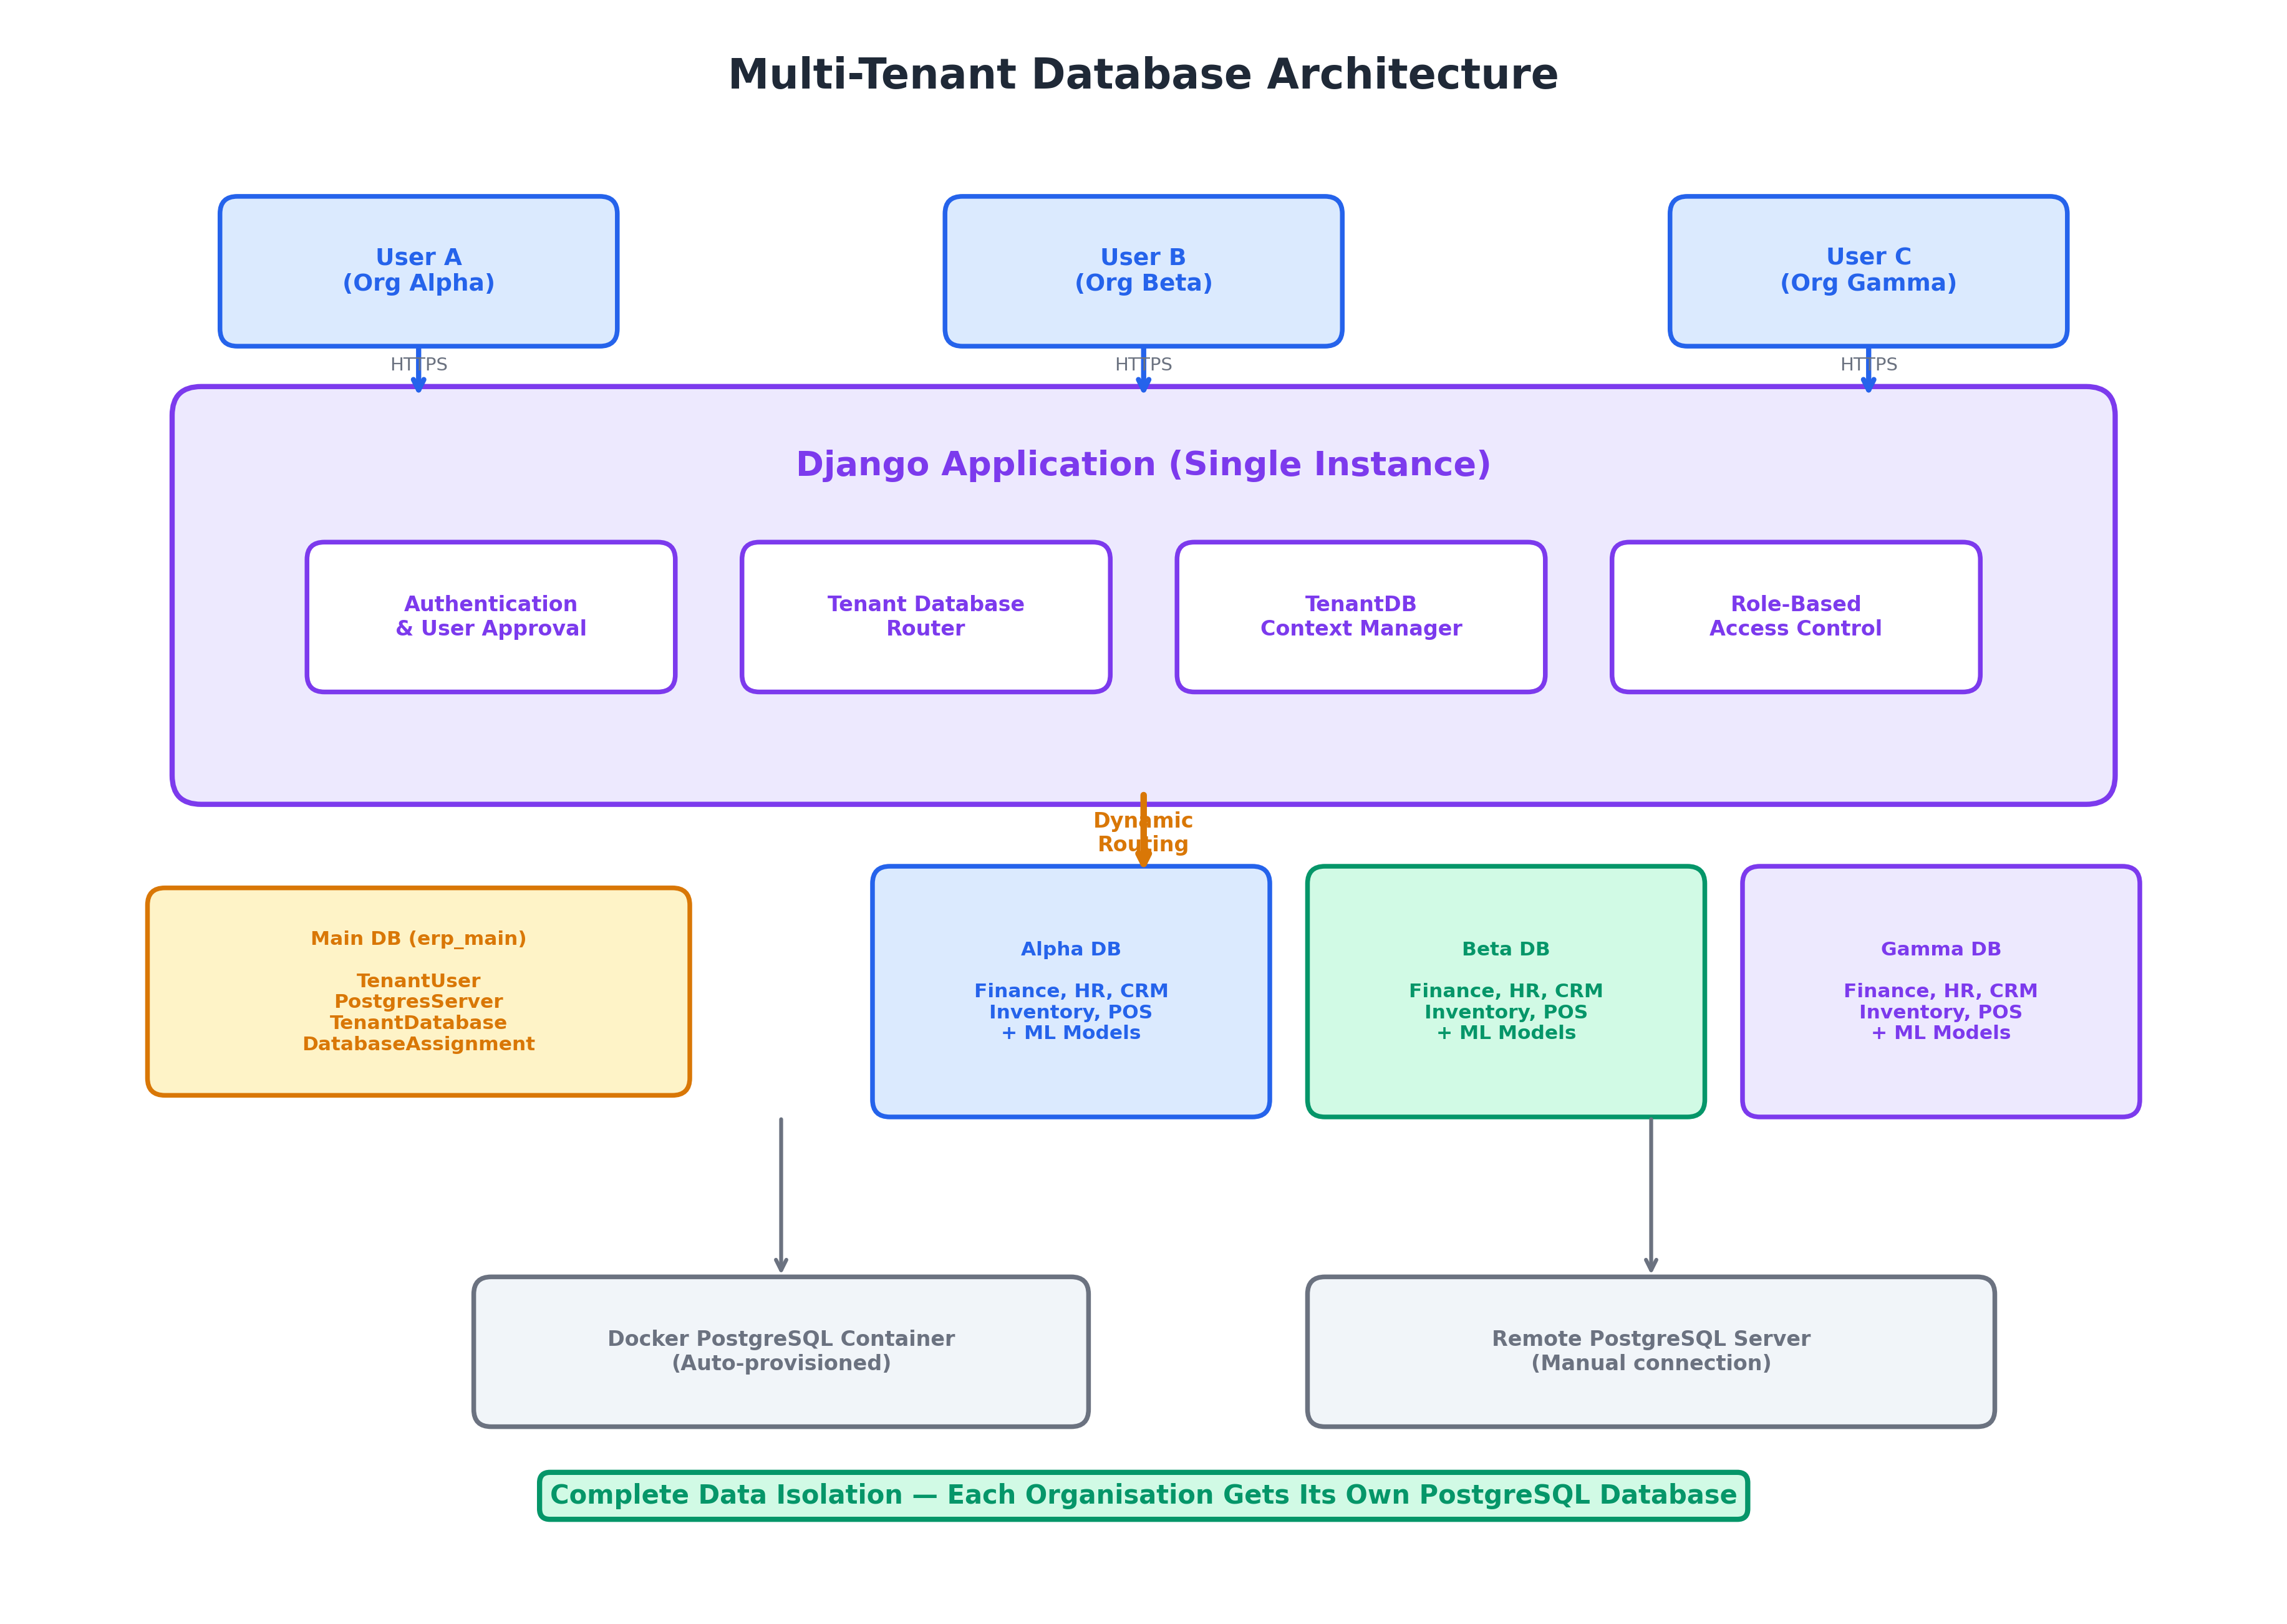
\includegraphics[width=0.95\textwidth]{figures/multi_tenant_architecture.png}
    \caption{Database-per-tenant architecture with dynamic PostgreSQL provisioning}
    \label{fig:multi_tenant_arch}
\end{figure}

The database routing mechanism works as follows:

\begin{enumerate}[label=\arabic*.]
  \item The user logs in and the authentication middleware identifies their \texttt{DatabaseAssignment}.
  \item The \texttt{add\_tenant\_database()} function dynamically registers the tenant's database connection parameters in Django's \texttt{DATABASES} dictionary.
  \item The \texttt{TenantDatabaseContext} context manager sets the active database alias for the current request thread.
  \item All subsequent ORM queries are automatically routed to the tenant's database via the custom \texttt{DATABASE\_ROUTERS} configuration.
  \item When the request completes, the context manager resets the routing.
\end{enumerate}

\subsection{AI/ML Pipeline Architecture}

The ML pipeline is integrated into the ERP as a self-contained module (\texttt{erp.ai}) with the following components:

\begin{itemize}
  \item \textbf{Model Registry} (\texttt{MLModel}): Tracks model versions, accuracy scores, training parameters, and artefact file paths. Each model is scoped to a specific company (tenant).

  \item \textbf{Service Layer} (\texttt{erp.ai.services}): Contains the implementation of each ML model as a Python class. Each service class follows a consistent interface: \texttt{train()}, \texttt{predict()}, and an optional \texttt{score\_all()} batch method.

  \item \textbf{Explainability Service} (\texttt{erp.ai.services.explainability}): The XAI module, encapsulated in the \texttt{ExplainabilityService} class.  It provides:
  \begin{itemize}
    \item \texttt{explain\_prediction()} --- Instance-level SHAP or LIME explanation for a single entity (invoice, lead, or employee), returning feature contributions, base values, top-feature rankings, and waterfall plot data.
    \item \texttt{global\_feature\_importance()} --- Global SHAP analysis using a background sample (up to 200 instances), producing mean~$|\text{SHAP}|$ importance rankings, beeswarm data, and summary plots (base64-encoded PNG).
    \item \texttt{get\_explanation\_history()} --- Retrieval of persisted explanations from the \texttt{ExplanationResult} model with optional filters by model type, entity, or method.
  \end{itemize}
  Internally, the service dispatches to \texttt{\_shap\_explain()} (using \texttt{shap.TreeExplainer}) for tree-based models (GBM, Random Forest) and \texttt{\_lime\_explain()} (using \texttt{lime.lime\_tabular.LimeTabularExplainer}) for model-agnostic fallback. It handles SHAP version differences (2D vs.\ 3D output arrays), scalar vs.\ array expected values, and applies artefact scalers when present.

  \item \textbf{Explanation Result Model} (\texttt{ExplanationResult}): Persists each explanation with the entity type, entity ID, explanation method (SHAP/LIME), prediction score, feature contributions (JSON), and top features for audit and historical analysis.

  \item \textbf{Training Pipeline} (\texttt{train\_models} management command): An orchestrator that sequentially trains all selected models, evaluates their performance, and generates a JSON training report.

  \item \textbf{Prediction Logging} (\texttt{PredictionLog}): An immutable audit trail of every prediction made, enabling future retraining on actual outcomes.

  \item \textbf{AI Insight Engine} (\texttt{AIInsight} + \texttt{create\_or\_update\_insight}): Converts ML model outputs into human-readable alerts with severity levels, recommendations, and action URLs. Includes automatic deduplication via a configurable cooldown window.
\end{itemize}

\begin{figure}[H]
    \centering
    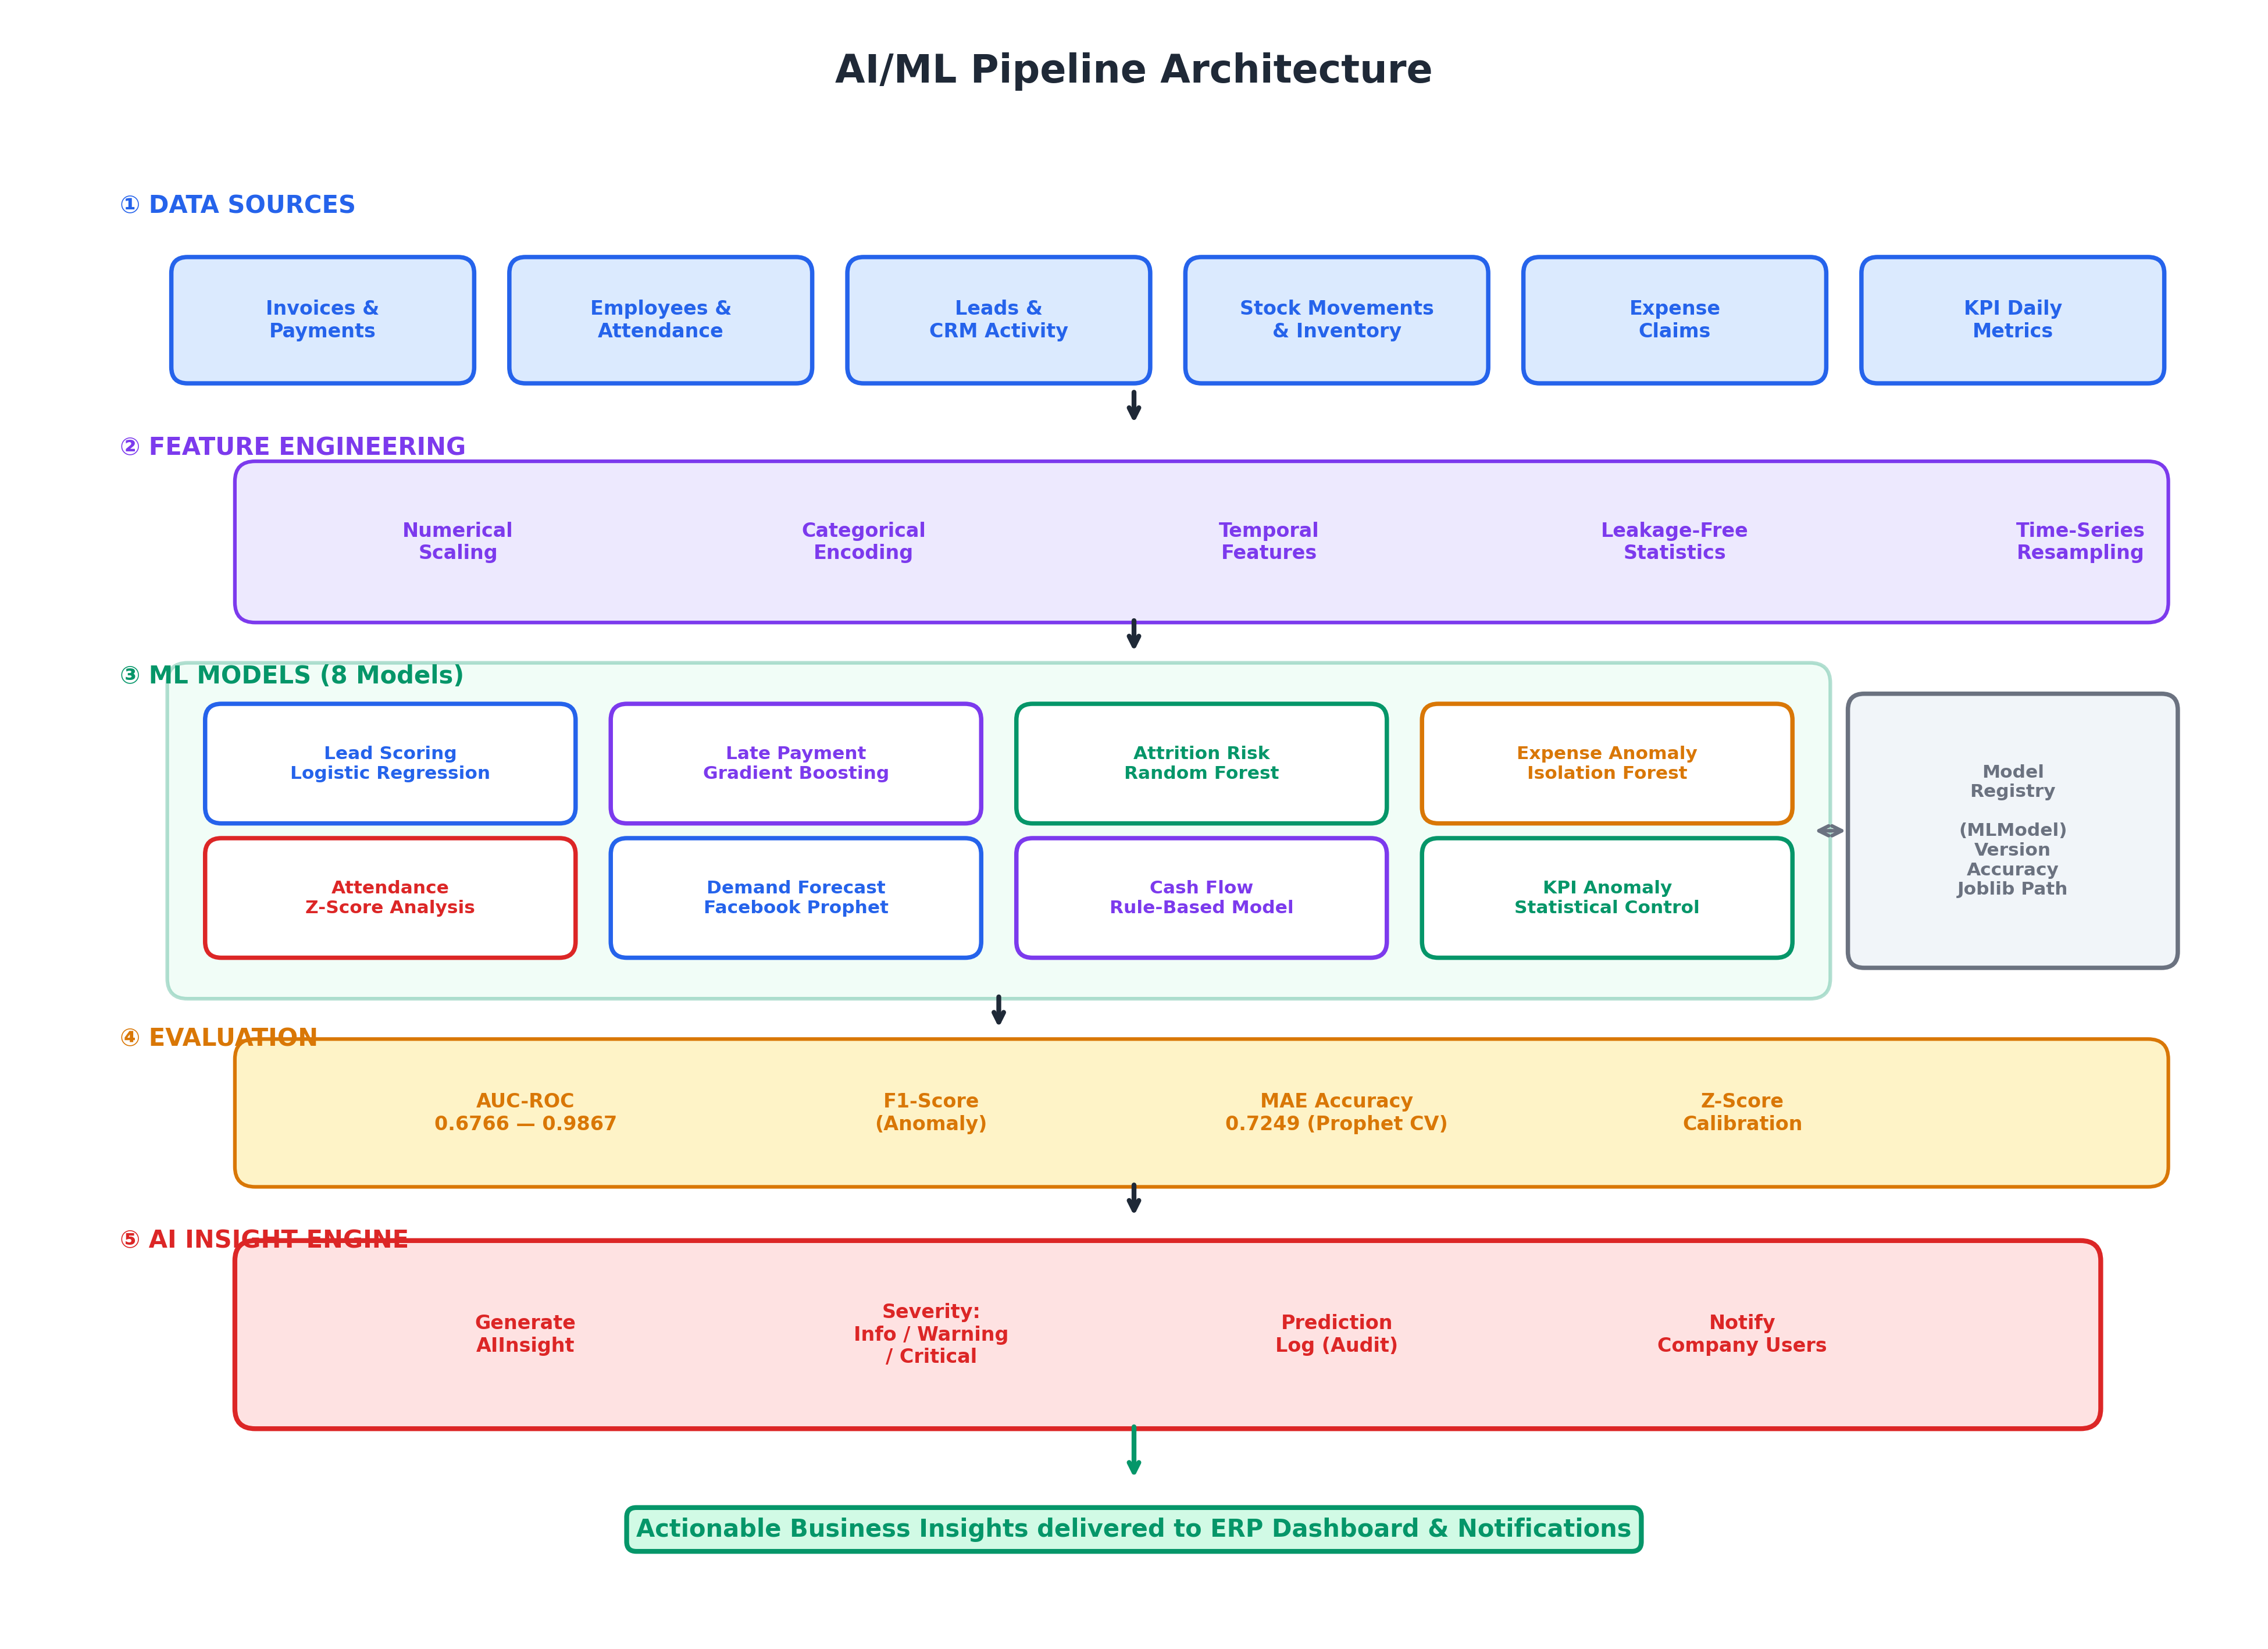
\includegraphics[width=0.95\textwidth]{figures/ml_pipeline_architecture.png}
    \caption{AI/ML pipeline architecture showing the flow from raw data to actionable insights}
    \label{fig:ml_pipeline}
\end{figure}


\section{Technology Stack}
\label{sec:tech_stack}

Table~\ref{tab:tech_stack} summarizes the technologies used in this project:

\begin{table}[H]
\centering
\caption{Technology stack}
\label{tab:tech_stack}
\begin{tabularx}{\textwidth}{l l >{\raggedright\arraybackslash}X}
\toprule
\textbf{Layer} & \textbf{Technology} & \textbf{Purpose} \\
\midrule
Backend Framework & Django 4.2 & Web framework, ORM, URL routing, template engine \\
Programming Language & Python 3.12 & Primary development language \\
Database & PostgreSQL 12+ & Relational database for main and tenant databases \\
REST API & Django REST Framework 3.14 & RESTful API layer for mobile/third-party integration \\
ML / Data Science & scikit-learn 1.4, pandas 2.0, numpy 1.26 & Classical ML algorithms and data processing \\
Explainable AI & SHAP 0.51, LIME 0.2, matplotlib 3.10 & SHAP TreeExplainer, LIME TabularExplainer, summary plots \\
Time-Series Forecasting & Facebook Prophet 1.1.5 & Additive regression for demand forecasting \\
LLM Integration & OpenAI API (GPT-4o-mini) & AI assistant and natural language analysis \\
Task Queue & Celery 5.3 + Redis 5.0 & Asynchronous ML training and background jobs \\
Containerization & Docker + docker-py 6.1 & Dynamic PostgreSQL server provisioning \\
Frontend & Django Templates + Bootstrap 5 + Crispy Forms & Server-side rendered responsive UI \\
PDF Generation & xhtml2pdf 0.2 & Invoice and report PDF export \\
Data Visualization & Plotly 5.22 & Interactive charts and dashboards \\
Version Control & Git + GitHub & Source code management \\
Deployment & Gunicorn 21.2 & WSGI HTTP server for production \\
\bottomrule
\end{tabularx}
\end{table}


\section{Data Collection and Preparation}
\label{sec:data_collection}

The ML models in this project are trained on a combination of real-world open-source datasets and synthetic domain-specific data generated to fill coverage gaps:

\subsection{Open-Source Datasets}

\begin{enumerate}[label=\arabic*.]
  \item \textbf{Olist Brazilian E-Commerce Dataset} \citep{olist2018}: A public dataset from Kaggle containing over 100,000 real e-commerce orders from Brazilian marketplaces (2016--2018). This dataset provides:
  \begin{itemize}
    \item 99,441 orders with order dates, delivery dates, and payment information
    \item 32,216 products across 73 categories
    \item 96,096 customers with geolocation data
    \item 3,095 sellers
  \end{itemize}
  The Olist dataset was used to populate the Customers, Products, Invoices, Orders, and Payments modules.

  \item \textbf{IBM HR Employee Attrition Dataset} \citep{ibm2017hr}: A synthetic but statistically realistic dataset of 1,470 employee records with 35 attributes including salary, department, overtime hours, and attrition labels. This dataset trains the Employee Attrition Prediction model.

  \item \textbf{Supplier Procurement Dataset}: A custom-generated dataset of 50 suppliers and 873 purchase orders with realistic procurement cycles, used to populate the Supplier and Purchase Order modules.

  \item \textbf{Attendance Timeseries Dataset}: A custom-generated dataset of employee attendance records spanning 12 months with check-in/check-out times, hours worked, late arrival flags, and overtime hours.

  \item \textbf{Expense Claims Dataset}: A custom-generated dataset of 6,278 approved expense claims with embedded anomalies (labeled \texttt{is\_anomaly} column) for Isolation Forest evaluation.

  \item \textbf{CRM Leads Dataset}: A custom-generated dataset of 4,062 leads with source, estimated value, activities, and won/lost outcomes.
\end{enumerate}

\subsection{Synthetic Data Generation}

For modules without corresponding real-world datasets---particularly Inventory/WMS and KPI monitoring---a data seeding utility (\texttt{seed\_ml\_operational\_data}) was developed. This management command generates:

\begin{itemize}
  \item \textbf{Stock Movements:} 365 days of daily demand history for 80 products with weekly and monthly seasonality, product diversity profiles (fast/moderate/slow movers), weekend dips, growth trends, and random noise.

  \item \textbf{Reorder Rules:} 80 product-warehouse rule configurations with randomized lead times, safety stock levels, and minimum order quantities.

  \item \textbf{Supplier Invoices:} 220 pending supplier invoices with due dates spanning the next 90 days for Cash Flow projection.

  \item \textbf{KPI Spike Injection:} Calibrated inventory movement spikes targeting z-score $\approx 3.5\sigma$ above the 90-day baseline for KPI Anomaly Detection testing.
\end{itemize}


\section{Machine Learning Model Design}
\label{sec:ml_design}

\subsection{Model Selection Criteria}

The ML models were selected based on four criteria:

\begin{enumerate}[label=\arabic*.]
  \item \textbf{Interpretability:} Business users must understand why a prediction was made. Models with native feature importance (Random Forest, Gradient Boosting) and calibrated probabilities (Logistic Regression) were preferred.

  \item \textbf{Data Efficiency:} SME datasets are typically small (hundreds to low thousands of records). Models that perform well with limited data (Prophet, Z-Score, Isolation Forest) were favored.

  \item \textbf{Operational Simplicity:} Models must train in seconds to minutes on a standard server, serialize as compact files (joblib), and produce predictions with sub-second latency.

  \item \textbf{Task Appropriateness:} Each algorithm was matched to its problem type---classification (Logistic Regression, GBM, Random Forest), unsupervised anomaly detection (Isolation Forest, Z-Score), time-series forecasting (Prophet), and rule-based projection (Cash Flow).
\end{enumerate}

\subsection{Model Specifications}

Table~\ref{tab:ml_models} summarizes the eight ML models implemented in this project:

\begin{longtable}{p{2.5cm} p{2cm} p{2.5cm} p{2.5cm} p{2cm} p{1.5cm}}
\caption{ML model specifications} \label{tab:ml_models} \\
\toprule
\textbf{Model} & \textbf{Domain} & \textbf{Algorithm} & \textbf{Features} & \textbf{Evaluation Metric} & \textbf{Min. Samples} \\
\midrule
\endfirsthead
\caption[]{ML model specifications (continued)} \\
\toprule
\textbf{Model} & \textbf{Domain} & \textbf{Algorithm} & \textbf{Features} & \textbf{Evaluation Metric} & \textbf{Min. Samples} \\
\midrule
\endhead
Lead Scoring & CRM & Logistic Regression (C=1.0) & 7 features (value, age, activities, source, contact info) & AUC-ROC & 30 \\
\addlinespace
Late Payment & Finance & Gradient Boosting (300 trees, depth=5, lr=0.08) & 10 features (amount, days-to-due, customer history) & AUC-ROC & 30 \\
\addlinespace
Attrition & HR & Random Forest (300 trees, depth=8, balanced) & 10 features (tenure, salary, attendance, overtime) & AUC-ROC & 30 \\
\addlinespace
Expense Anomaly & Finance & Isolation Forest (300 trees, contamination=3\%) & 4 features (amount, month, weekday, category) & F1-Score vs. ground truth & 30 \\
\addlinespace
Attendance Anomaly & HR & Z-Score (threshold=2.0) & 2 metrics (avg hours, late arrival ratio) & Anomaly count & 1 \\
\addlinespace
Demand Forecast & Inventory & Prophet (additive, weekly + monthly seasonality) & Daily demand history per product/warehouse & MAE-based accuracy via cross-validation & 30 \\
\addlinespace
Cash Flow & Finance & Rule-based (30/60/90-day projection) & Outstanding invoices + pending payables + open POs & Net cash position & 0 \\
\addlinespace
KPI Anomaly & Operations & Z-Score (threshold $\geq 2\sigma$ warning, $\geq 3\sigma$ critical) & 5 daily KPIs (revenue, expenses, leads, overdue invoices, inventory movements) & Alert accuracy & 14 \\
\bottomrule
\end{longtable}

\subsection{Model Evaluation Strategy}

Each model is evaluated using appropriate metrics for its task type:

\begin{itemize}
  \item \textbf{Classifiers} (Lead Scoring, Late Payment, Attrition): AUC-ROC on a stratified 80/20 train/test split. AUC-ROC is preferred over accuracy because the datasets exhibit class imbalance.

  \item \textbf{Anomaly Detectors} (Expense Anomaly): Precision, Recall, and F1-Score computed against a ground-truth \texttt{is\_anomaly} label in the expense dataset.

  \item \textbf{Time-Series Forecasts} (Demand): MAE-based accuracy ($1 - \frac{MAE}{\bar{y}}$) computed via Prophet's built-in cross-validation with expanding windows.

  \item \textbf{Statistical Detectors} (Attendance Anomaly, KPI Anomaly): Qualitative evaluation based on the number of alerts generated and their clinical reasonableness (e.g., z-score magnitude aligning with injected anomalies).

  \item \textbf{Cash Flow}: Validation against known payables and receivables in the database---checking that inflows equal outstanding invoice balances and outflows match pending supplier invoices.
\end{itemize}

\subsection{XAI Evaluation Methodology}
\label{sec:xai_eval_methodology}

The Explainable AI module is evaluated along four dimensions:

\begin{enumerate}[label=\arabic*.]
  \item \textbf{Explanation Validity (Additivity):} For SHAP explanations, the sum of all feature attributions plus the base value must equal the predicted probability (Equation~\ref{eq:shapley}). Any deviation exceeding $\pm0.01$ indicates a computational error. This property is verified programmatically for every instance-level explanation.

  \item \textbf{Feature Coherence (Global):} For each model, the global SHAP feature importance distribution is analysed:
  \begin{itemize}
    \item The fraction of total importance held by the top feature is measured. A healthy model should spread importance across multiple features; dominance above 50\% triggers a data-leakage investigation.
    \item The number of features with non-zero mean $|\text{SHAP}|$ is counted. If the model ignores most features (zero SHAP), the feature engineering may be deficient.
  \end{itemize}

  \item \textbf{Cross-Method Agreement:} For a set of representative instances, the top-5 features from SHAP and the top-5 features from LIME are compared. The overlap ratio (Jaccard similarity) quantifies explanation consistency. High agreement ($\geq 3/5$) increases confidence; low agreement ($\leq 1/5$) signals local non-linearity or LIME approximation instability.

  \item \textbf{Data-Leakage Detection:} SHAP importance analysis is used to detect two types of leakage:
  \begin{itemize}
    \item \textit{Temporal leakage:} Features computed using future information relative to the prediction timestamp (e.g., \texttt{days\_since\_created} for historical leads).
    \item \textit{Proxy-target leakage:} Features that encode the target variable through a correlated proxy (e.g., \texttt{payroll\_months} correlating with employment status).
  \end{itemize}
\end{enumerate}


\section{Development Tools and Environment}
\label{sec:dev_tools}

\begin{table}[H]
\centering
\caption{Development tools and environment}
\label{tab:dev_tools}
\begin{tabularx}{\textwidth}{l l >{\raggedright\arraybackslash}X}
\toprule
\textbf{Category} & \textbf{Tool} & \textbf{Purpose} \\
\midrule
IDE & Visual Studio Code & Primary code editor with Python and Django extensions \\
AI Pair Programming & GitHub Copilot (Claude) & AI-assisted code generation and debugging \\
Version Control & Git + GitHub & Source code management and collaboration \\
Database Client & pgAdmin 4 & PostgreSQL database management and querying \\
API Testing & Django REST Framework browsable API & Interactive API testing and documentation \\
Virtual Environment & Python venv & Dependency isolation \\
Operating System & Windows 11 & Development machine OS \\
Browser & Google Chrome DevTools & Frontend debugging and responsive design testing \\
\bottomrule
\end{tabularx}
\end{table}


\section{Summary}
\label{sec:meth_summary}

This chapter detailed the Sprint (Agile) methodology adopted for the project, breaking the development into eight two-week Sprints covering platform architecture through XAI evaluation and deployment. The three-tier system architecture with database-per-tenant multi-tenancy was described, along with the AI/ML pipeline that trains, evaluates, logs, and surfaces model outputs as actionable business insights, augmented by an Explainability Service that provides SHAP and LIME explanations. The technology stack centres on Django 4.2, PostgreSQL, scikit-learn, SHAP 0.51, LIME 0.2, and Facebook Prophet. Data collection combines six real-world and synthetic datasets totalling over 140,000 records across five business domains. The XAI evaluation methodology was defined with four dimensions: explanation validity, feature coherence, cross-method agreement, and data-leakage detection. The following chapter presents the detailed system analysis and design, including use case diagrams, class diagrams, and database schema design.


% ██████████████████████████████████████████████████████████████████
%
%  CHAPTER 4 — SYSTEM ANALYSIS AND DESIGN
%
% ██████████████████████████████████████████████████████████████████
\chapter{System Analysis and Design}
\label{ch:analysis_design}

\section{Introduction}
\label{sec:ad_intro}

This chapter presents the functional and non-functional requirements, use case modelling, class design, database schema, and the XAI pipeline architecture that together define the system's blueprint. The design builds on the architectural decisions described in Chapter~3 and provides the specification from which the implementation (Chapter~5) was realised.

\section{Functional Requirements}
\label{sec:functional_req}

The system's functional requirements are organised into three tiers: platform-level, ERP-module-level, and AI/XAI-level.

\subsection{Platform Requirements}

\begin{longtable}{c p{3cm} p{8cm}}
\caption{Platform-level functional requirements} \label{tab:platform_req} \\
\toprule
\textbf{ID} & \textbf{Requirement} & \textbf{Description} \\
\midrule
\endfirsthead
\toprule
\textbf{ID} & \textbf{Requirement} & \textbf{Description} \\
\midrule
\endhead
FR-01 & User Registration & Users can register with email, password, company name, and optional preferred language. \\
FR-02 & Tenant Approval & An administrator can approve or reject pending tenant registrations. \\
FR-03 & Database Provisioning & Approved tenants trigger automatic PostgreSQL database creation on a configured server (Docker or remote). \\
FR-04 & Role-Based Access & Four roles (Owner, Admin, User, Read-Only) control access to ERP functions within a tenant. \\
FR-05 & Tenant Switching & Users with multiple database assignments can switch between tenant contexts. \\
FR-06 & Session Isolation & Each request is routed to the correct tenant database via middleware and context managers. \\
\bottomrule
\end{longtable}

\subsection{AI/XAI Requirements}

\begin{longtable}{c p{3cm} p{8cm}}
\caption{AI and XAI functional requirements} \label{tab:ai_xai_req} \\
\toprule
\textbf{ID} & \textbf{Requirement} & \textbf{Description} \\
\midrule
\endfirsthead
\toprule
\textbf{ID} & \textbf{Requirement} & \textbf{Description} \\
\midrule
\endhead
FR-20 & Model Training & Admin users can trigger ML model training via a management command or Celery task. \\
FR-21 & Model Versioning & The system maintains a version history of trained models with accuracy metrics. \\
FR-22 & Batch Scoring & All eligible entities (invoices, leads, employees) can be scored in batch after training. \\
FR-23 & AI Insights & Model outputs are converted into human-readable alerts (Info, Warning, Critical) and displayed in the ERP dashboard. \\
FR-24 & \textbf{Instance Explanation} & Users can request a SHAP or LIME explanation for any individual prediction (invoice, lead, employee). \\
FR-25 & \textbf{Global Importance} & Users can view the global SHAP feature importance ranking for any trained model. \\
FR-26 & \textbf{Explanation History} & All explanations are persisted with timestamps, method, feature contributions, and prediction scores for audit. \\
FR-27 & \textbf{XAI Visualisation} & Waterfall plots, beeswarm charts, and feature-contribution tables are rendered via Plotly in the web interface. \\
FR-28 & \textbf{XAI API} & REST endpoints expose instance explanation, global importance, and explanation history for third-party integration. \\
\bottomrule
\end{longtable}

\section{Non-Functional Requirements}
\label{sec:nonfunctional_req}

\begin{longtable}{c p{3cm} p{8cm}}
\caption{Non-functional requirements} \label{tab:nonfunc_req} \\
\toprule
\textbf{ID} & \textbf{Requirement} & \textbf{Description} \\
\midrule
\endfirsthead
\toprule
\textbf{ID} & \textbf{Requirement} & \textbf{Description} \\
\midrule
\endhead
NFR-01 & Data Isolation & Tenant data must be physically separated in dedicated PostgreSQL databases; cross-tenant queries must be impossible. \\
NFR-02 & Response Time & SHAP instance explanations must complete within 5 seconds; LIME within 10 seconds; global SHAP within 30 seconds. \\
NFR-03 & Scalability & The system must support 50+ concurrent tenants on a single application server. \\
NFR-04 & Explanation Determinism & SHAP explanations for the same input must produce identical results across runs (deterministic). LIME explanations may vary within stochastic bounds. \\
NFR-05 & Bilingual Support & All UI labels, model fields, and XAI feature names must be available in English and Arabic. \\
NFR-06 & Auditability & Every prediction and explanation is logged immutably for regulatory compliance. \\
NFR-07 & Portability & The system runs on any OS with Python 3.12+ and PostgreSQL 12+. \\
\bottomrule
\end{longtable}

\section{Use Case Design}
\label{sec:use_cases}

\subsection{XAI Use Cases}

The XAI module introduces three primary use cases:

\begin{enumerate}[label=\textbf{UC-XAI-\arabic*:}]
  \item \textbf{Explain Single Prediction:} The user selects an entity (e.g., Invoice \#1042) and requests an explanation. The system retrieves the trained model artefact, constructs the feature vector, invokes SHAP TreeExplainer (or LIME as fallback), and returns the waterfall plot data with ranked feature contributions.

  \item \textbf{View Global Feature Importance:} The user selects a model type (e.g., Late Payment). The system samples up to 200 background instances, computes mean~$|\text{SHAP}|$ values for each feature, and renders a beeswarm chart and bar plot.

  \item \textbf{Compare SHAP vs.\ LIME:} The user requests both explanation methods for the same entity. The system runs SHAP and LIME in sequence and displays the results side-by-side, highlighting agreement and divergence in top-5 feature rankings.
\end{enumerate}

\begin{figure}[H]
    \centering
    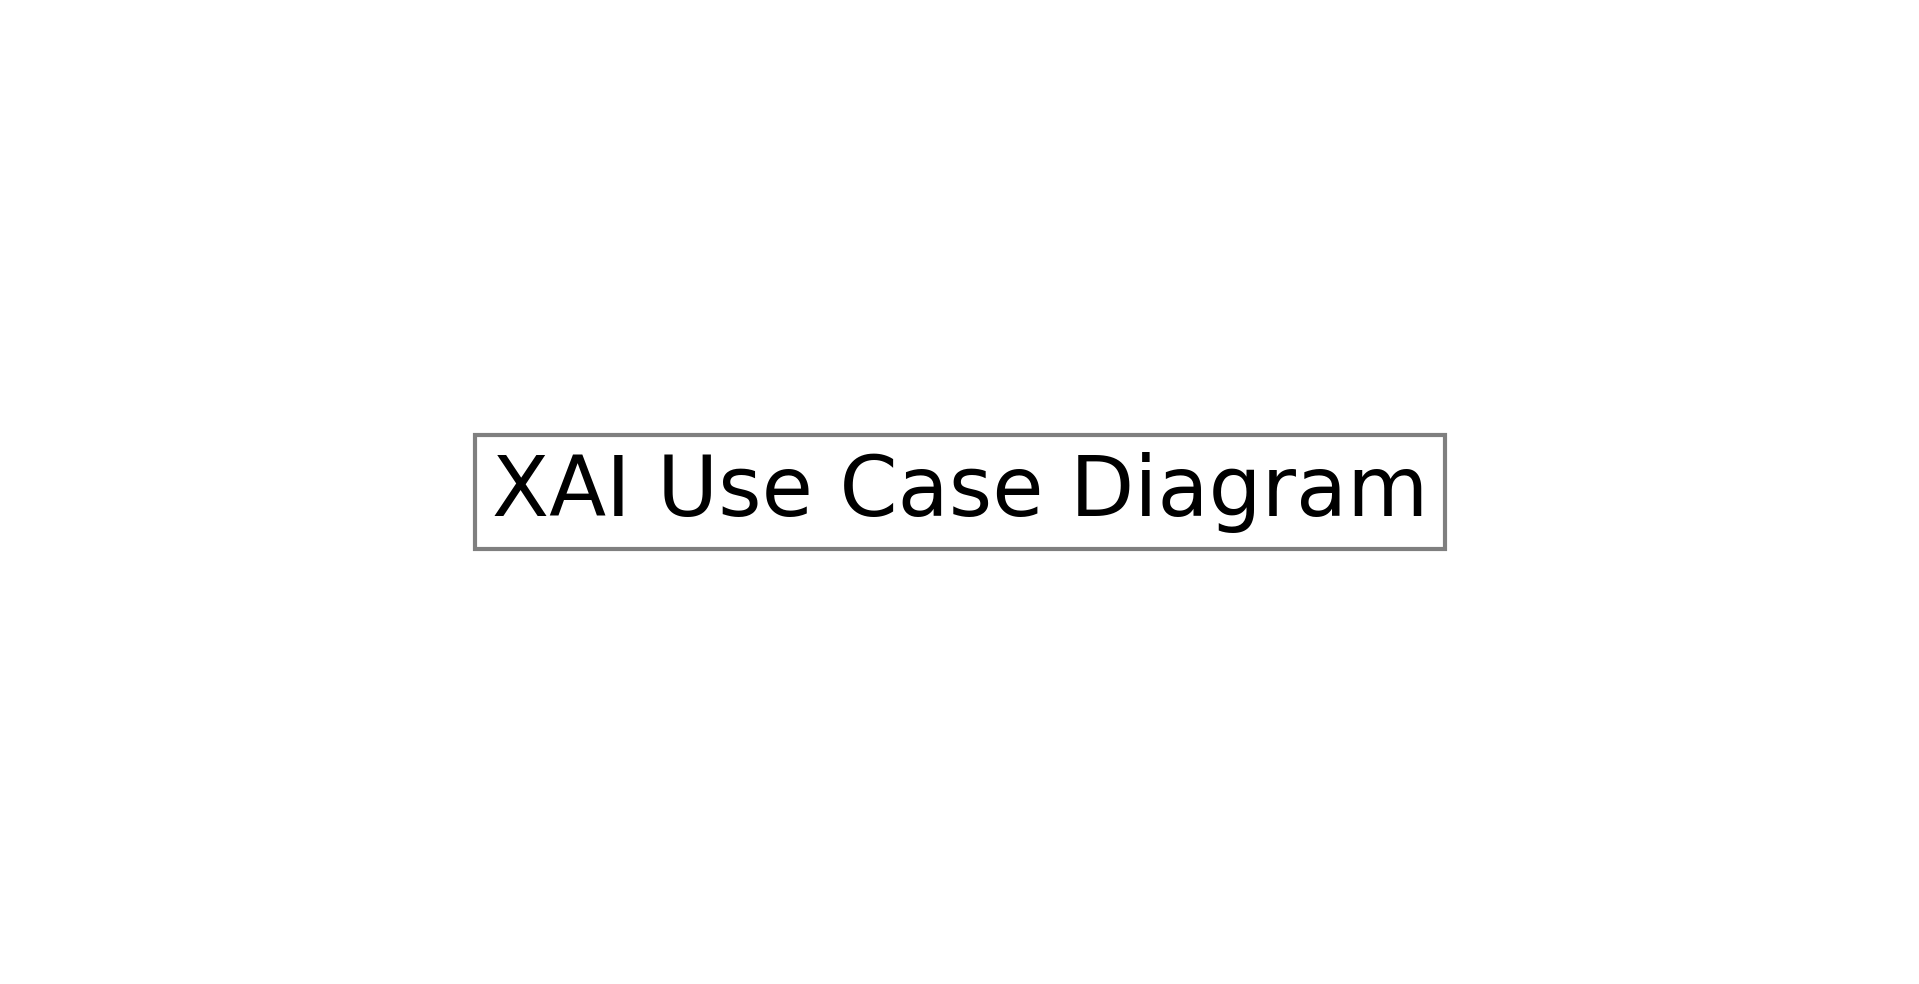
\includegraphics[width=0.85\textwidth]{figures/xai_use_case_diagram.png}
    \caption{Use case diagram for the Explainable AI module}
    \label{fig:xai_use_case}
\end{figure}

\section{XAI Class Design}
\label{sec:xai_class_design}

The XAI module follows a layered design pattern:

\begin{itemize}
  \item \textbf{Service Layer} (\texttt{ExplainabilityService}): Stateless class instantiated with a \texttt{company} object. Orchestrates model loading, feature construction, explainer invocation, and result persistence.

  \item \textbf{Model Layer} (\texttt{ExplanationResult}): Django ORM model with fields for \texttt{model} (FK to \texttt{MLModel}), \texttt{entity\_type}, \texttt{entity\_id}, \texttt{method} (shap/lime), \texttt{prediction\_score}, \texttt{feature\_contributions} (JSONField), \texttt{top\_features} (JSONField), and \texttt{created\_at}.

  \item \textbf{Serialiser Layer} (\texttt{ExplanationResultSerializer}): DRF serialiser exposing explanation data via REST API.

  \item \textbf{View Layer}: Web views (\texttt{ExplainabilityDashboardView}, \texttt{ExplainPredictionView}, \texttt{GlobalImportanceView}) and API viewsets (\texttt{ExplainabilityViewSet}).
\end{itemize}

\begin{figure}[H]
    \centering
    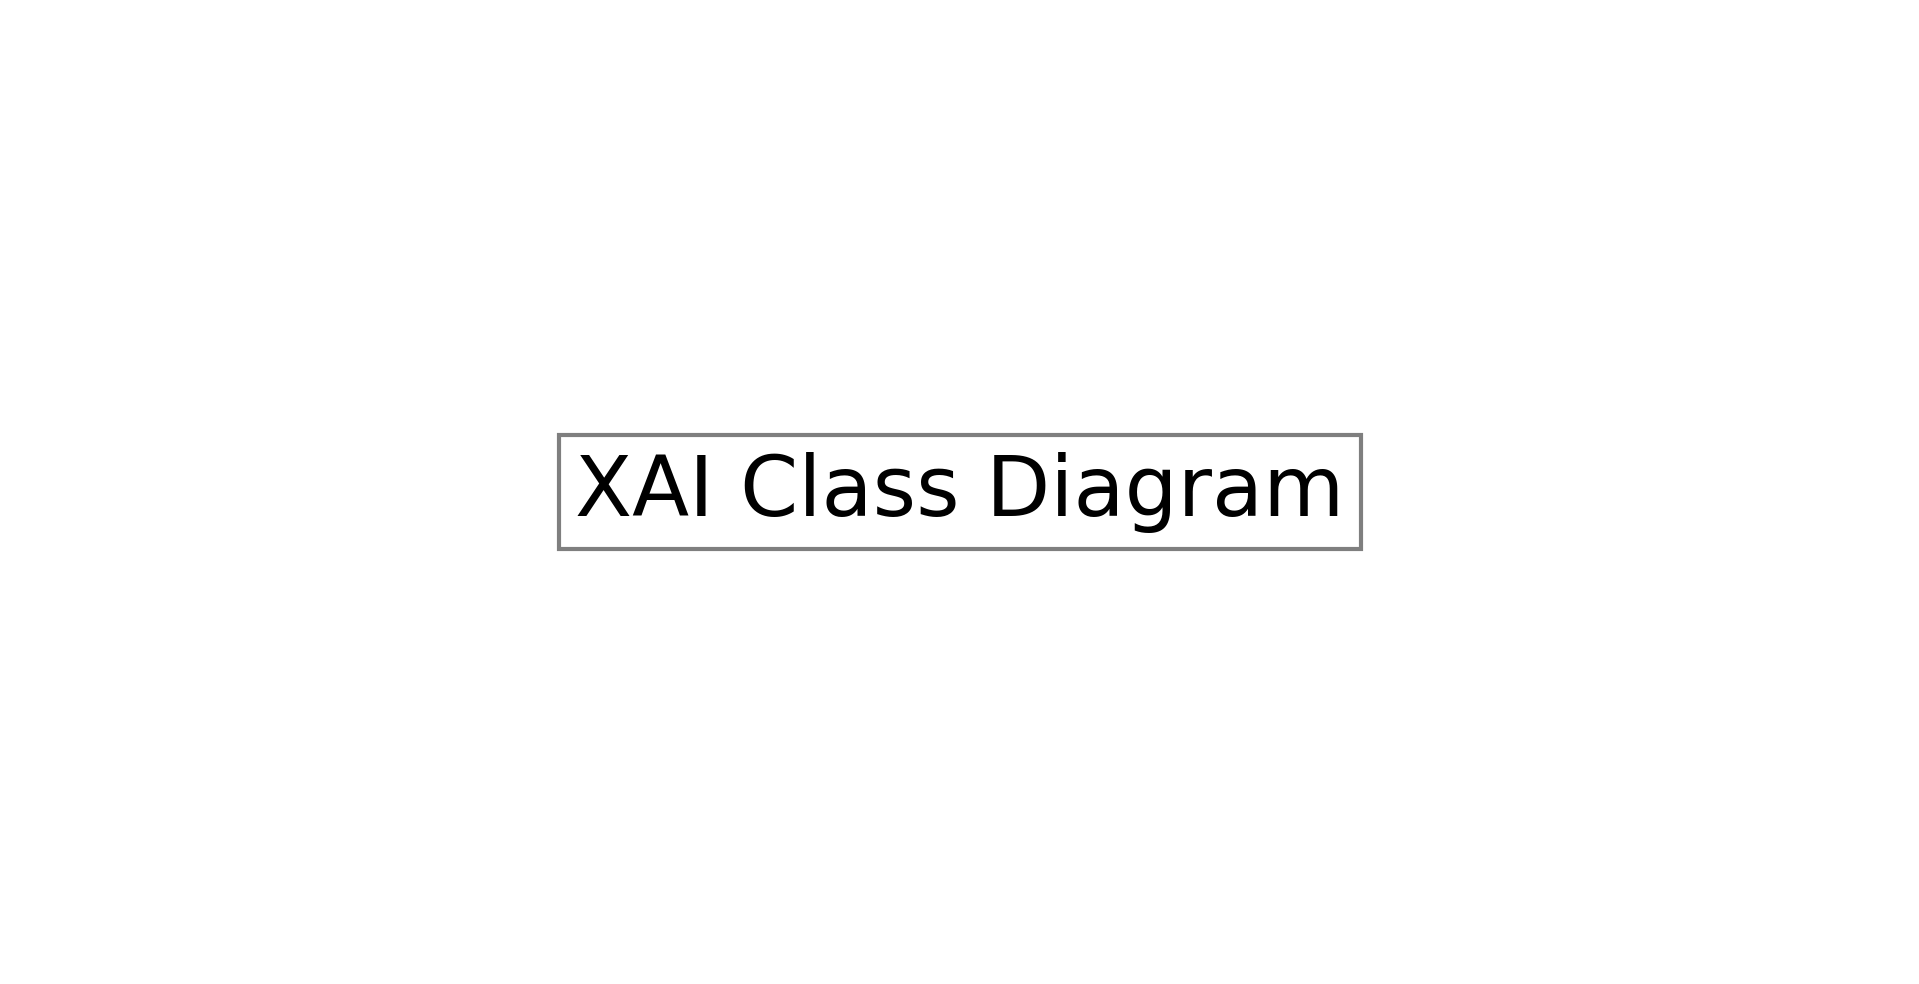
\includegraphics[width=0.85\textwidth]{figures/xai_class_diagram.png}
    \caption{Class diagram for the ExplainabilityService and related components}
    \label{fig:xai_class}
\end{figure}

\section{Database Schema Design}
\label{sec:db_schema}

\subsection{AI/XAI Schema}

The AI module adds the following tables to each tenant database:

\begin{table}[H]
\centering
\caption{AI/XAI database tables}
\label{tab:ai_schema}
\begin{tabularx}{\textwidth}{l l >{\raggedright\arraybackslash}X}
\toprule
\textbf{Table} & \textbf{Key Columns} & \textbf{Purpose} \\
\midrule
\texttt{ai\_mlmodel} & \texttt{model\_type}, \texttt{version}, \texttt{accuracy\_score}, \texttt{artefact\_path}, \texttt{parameters} (JSON) & Model registry: tracks trained model versions \\
\addlinespace
\texttt{ai\_predictionlog} & \texttt{model} (FK), \texttt{entity\_type}, \texttt{entity\_id}, \texttt{prediction\_score}, \texttt{features\_used} (JSON) & Immutable prediction audit trail \\
\addlinespace
\texttt{ai\_aiinsight} & \texttt{insight\_type}, \texttt{severity}, \texttt{title}, \texttt{message}, \texttt{action\_url}, \texttt{is\_read} & Human-readable ML alerts \\
\addlinespace
\texttt{ai\_explanationresult} & \texttt{model} (FK), \texttt{entity\_type}, \texttt{entity\_id}, \texttt{method}, \texttt{prediction\_score}, \texttt{feature\_contributions} (JSON), \texttt{top\_features} (JSON) & \textbf{Persisted SHAP/LIME explanations} \\
\bottomrule
\end{tabularx}
\end{table}

\section{XAI Pipeline Architecture}
\label{sec:xai_pipeline_design}

Figure~\ref{fig:xai_pipeline_flow} illustrates the flow of an explanation request through the system:

\begin{enumerate}[label=\arabic*.]
  \item The user clicks ``Explain'' on an entity page (or calls the API endpoint).
  \item The view layer invokes \texttt{ExplainabilityService.explain\_prediction()}.
  \item The service loads the model artefact (classifier + scaler + feature\_cols) from the \texttt{MLModel} registry.
  \item The feature vector is constructed by delegating to model-specific helper methods (e.g., \texttt{\_features\_late\_payment()}) that reuse the same feature engineering logic as the prediction service.
  \item For tree-based models, \texttt{shap.TreeExplainer} is initialised with the classifier and computes exact Shapley values. The 3D output array (for newer SHAP versions with binary classifiers) is handled by slicing the positive-class index.
  \item The base value (expected value of the positive class) is extracted, handling both scalar and array formats.
  \item Feature contributions are sorted by $|\text{SHAP value}|$ descending, annotated with direction (``increases''/``decreases'') and human-readable impact descriptions.
  \item Waterfall plot data (cumulative bar segments from base value to prediction) is computed for frontend rendering.
  \item The explanation is persisted to \texttt{ExplanationResult} and returned to the view/API.
\end{enumerate}

\begin{figure}[H]
    \centering
    
\includegraphics[width=0.95\textwidth]{figures/xai_pipeline_architecture.png}
    \caption{Data flow for instance-level SHAP/LIME explanation generation}
    \label{fig:xai_pipeline_flow}
\end{figure}

\section{Implemented System Capabilities}
\label{sec:capabilities}

To make the as-built scope explicit -- the platform has grown substantially since the initial Sprint plan -- this section enumerates the capabilities that are actually implemented and reachable in the current code base, organised by domain. Each bullet maps to a concrete Python module, Django app, REST endpoint, Celery task, or Flutter screen. Quantitative summary: 70+ ORM models across 13 model files, 40+ DRF \texttt{ModelViewSet}s, 78 form classes, 17 management commands, 23 Celery tasks (scheduled + async), 10 ML/AI service classes, a Flutter mobile app of 78 Dart files, and trilingual (Arabic / English / Indonesian) localisation with RTL support.

\subsection{Multi-Tenant Platform (\texttt{tenants/} app)}
\begin{itemize}
  \item \textbf{Database-per-tenant} with a custom router (\texttt{tenants/routers.py}, \texttt{TenantDatabaseRouter}) that pins \texttt{auth}, \texttt{tenants}, and \texttt{sessions} to the infrastructure DB while routing every ERP model to the tenant's database; the active alias is set via a thread-local helper (\texttt{set\_current\_db\_alias}).
  \item Models: \texttt{TenantUser} (email-based custom user with approval workflow: \emph{pending / approved / rejected / suspended}), \texttt{PostgresServer}, \texttt{TenantDatabase}, \texttt{DatabaseAssignment}, \texttt{ServerLog}, \texttt{EmployeeInviteLink}, \texttt{ScheduledTask}, \texttt{TaskExecution}, \texttt{AlertRule}, \texttt{Alert}, \texttt{TenantQuota}, \texttt{UsageSnapshot}, \texttt{Announcement}, \texttt{AnnouncementDismissal}, \texttt{MetricSnapshot}, \texttt{TicketCategory}, \texttt{Ticket}, \texttt{TicketMessage}, \texttt{TicketAttachment}.
  \item Dynamic provisioning of either \emph{Docker-managed} PostgreSQL containers or remote PostgreSQL servers, with health checks, restart, backup and restore from a dedicated platform-admin UI.
  \item \textbf{Platform-admin console} (\texttt{tenants/platform\_admin/}, 18~view files) covering users \& approvals, server management, database operations, monitoring/health, alerts, quotas, billing/usage, announcements, support tickets, scheduled tasks, mobile-app builds, backups, activity feed, Docker container introspection, and platform analytics.
  \item Tenant context is set at request time by \texttt{tenants.middleware.TenantMiddleware} from the user's \texttt{DatabaseAssignment} and propagated to every Celery task header so async ML jobs always run against the correct tenant DB.
  \item Quota enforcement (\texttt{TenantQuota} + \texttt{UsageSnapshot} + per-minute Celery refresh) and platform-wide announcements with per-user dismissal tracking.
\end{itemize}

\subsection{Core ERP Domain Models (70+ Django Models)}
\begin{itemize}
  \item \textbf{Core} (\texttt{erp/models/core.py}): \texttt{Currency}, \texttt{Company}, \texttt{Department}, \texttt{Branch}, \texttt{FiscalYear}, \texttt{Sequence}.
  \item \textbf{Base mixins} (\texttt{base.py}): \texttt{TimeStampedModel}, \texttt{AuditMixin}, \texttt{SoftDeleteMixin}/\texttt{SoftDeleteManager}, composed via \texttt{ERPBaseModel}.
  \item \textbf{Finance}: \texttt{Account}, \texttt{TaxRate}, \texttt{PaymentMethod}, \texttt{Customer}, \texttt{Invoice}/\texttt{InvoiceLine}, \texttt{Payment}/\texttt{PaymentAllocation} (multi-invoice allocation), \texttt{Expense}/\texttt{ExpenseCategory}/\texttt{ExpenseAttachment}, \texttt{JournalEntry}/\texttt{JournalEntryLine} (debit/credit posting).
  \item \textbf{HR / Payroll}: \texttt{Employee}, \texttt{EmployeeDocument}, \texttt{LeaveType}, \texttt{LeaveRequest}, \texttt{Attendance}, \texttt{Payroll}/\texttt{PayrollEarning}/\texttt{PayrollDeduction}, \texttt{AttendanceDevice} (RFID/biometric).
  \item \textbf{CRM}: \texttt{Lead}, \texttt{LeadActivity}, \texttt{CustomerInteraction}, \texttt{Campaign}, \texttt{CampaignLead}, \texttt{Task}, \texttt{TaskComment}.
  \item \textbf{Suppliers \& Procurement}: \texttt{Supplier}, \texttt{SupplierContact}, \texttt{SupplierDocument}, \texttt{PurchaseOrder}/\texttt{PurchaseOrderLine}, \texttt{SupplierInvoice}/\texttt{SupplierInvoiceLine}, \texttt{SupplierPayment}/\texttt{SupplierPaymentAllocation}.
  \item \textbf{Inventory \& WMS}: \texttt{UnitOfMeasure}/\texttt{UnitOfMeasureConversion}, \texttt{Warehouse}/\texttt{WarehouseZone}/\texttt{WarehouseBin}, \texttt{LotBatch}, \texttt{SerialNumber}, \texttt{StockItem}, \texttt{StockMovement} (immutable ledger), \texttt{GoodsReceiptNote}/\texttt{GoodsReceiptLine}, \texttt{StockTransfer}, \texttt{StockAdjustment}, \texttt{CycleCount}/\texttt{CycleCountLine} with variance posting, \texttt{PickList}, \texttt{ShipmentNote}, \texttt{ReorderRule}, \texttt{InventoryValuationConfig} (FIFO / Weighted Average / LIFO).
  \item \textbf{Services \& Products}: \texttt{ServiceCategory}, \texttt{ServicePricing}/\texttt{PriceTier}, \texttt{ServicePackage}/\texttt{PackageItem}, \texttt{Quote}/\texttt{QuoteLine}, \texttt{ProductCategory}, \texttt{Product}, \texttt{ProductSupplier}.
  \item \textbf{Fixed Assets}: \texttt{AssetCategory}, \texttt{FixedAsset}, \texttt{DepreciationSchedule}, \texttt{AssetDisposal}, \texttt{AssetTransfer}, \texttt{AssetRevaluation}, \texttt{AssetMaintenanceLog}.
  \item \textbf{POS}: \texttt{POSTerminal}, \texttt{POSSession} (open$\to$close shift), \texttt{POSOrder}/\texttt{POSOrderLine}, \texttt{POSPayment} (split-tender).
  \item \textbf{Reporting}: \texttt{ReportTemplate}, \texttt{GeneratedReport}, \texttt{Dashboard}/\texttt{DashboardWidget}, \texttt{KPI}/\texttt{KPIValue}.
  \item \textbf{Audit \& System}: \texttt{AuditLog} (generic FK, immutable), \texttt{SystemSetting}, \texttt{Notification}, \texttt{EmailTemplate}, \texttt{FileAttachment}, \texttt{ScheduledTask}, \texttt{IntegrationLog}.
  \item \textbf{AI / ML}: \texttt{MLModel}, \texttt{PredictionLog}, \texttt{AIInsight}, \texttt{ExplanationResult}, \texttt{AITrainingRun}.
\end{itemize}

\subsection{REST and Mobile API Surface}
\begin{itemize}
  \item Single SimpleRouter mounts 40+ \texttt{ModelViewSet}s under \texttt{/api/} for currencies, companies, departments, employees, leaves, attendance, payroll, customers, invoices, payments, expenses, suppliers, POs, leads, campaigns, tasks, services, quotes, every inventory entity (UoM, warehouses, zones, bins, lots, serials, stock items/movements, GRNs, transfers, adjustments, cycle counts, pick-lists, shipments, reorder rules), KPIs, dashboards, audit logs and notifications.
  \item Custom permission classes \texttt{IsCompanyUser} and \texttt{IsAIEnabled}; ViewSets inherit from a shared \texttt{ERPBaseViewSet} that injects company filtering, ordering and search.
  \item Financial reports API (\texttt{erp/api/reports\_views.py}): \texttt{TrialBalanceAPIView}, \texttt{ProfitAndLossAPIView}, \texttt{BalanceSheetAPIView}, \texttt{CashFlowAPIView}.
  \item AI/ML API (\texttt{erp/ai/api/}): \texttt{MLModelViewSet}, \texttt{PredictionLogViewSet}, \texttt{AIInsightViewSet}, \texttt{ExplanationResultViewSet}; trigger endpoints for lead-scoring, invoice-scoring, expense-anomaly, demand-forecast, attrition, KPI-checks; per-model retraining endpoints and a \emph{retrain-all} endpoint; \texttt{/api/ai/training/\{status,history,cancel\}/}; \texttt{/api/ai/cashflow/}; \texttt{/api/ai/assistant/} (LLM); \texttt{/api/ai/dashboard/}; \texttt{/api/ai/xai/explain/} and \texttt{/api/ai/xai/global/<model\_type>/}.
  \item \textbf{Mobile API} (\texttt{erp/api/mobile/}): query-optimised endpoints for the Flutter app (employee dashboard, attendance, leave requests, payslips, tasks, POS, admin dashboards/lists/approvals), documented in \texttt{docs/admin\_mobile\_api.md}.
\end{itemize}

\subsection{Server-Rendered Views and Templates}
\begin{itemize}
  \item 30 view modules under \texttt{erp/views/} covering: dashboard, customers, CRM, finance, HR, inventory, suppliers, employees, audit-log viewer, export, import, notifications, PDF generation, reports, tax report, journal posting, POS, products, services, fixed assets, attendance device pairing, employee portal, support tickets, UoM conversions, account balances, AJAX endpoints, plus a \texttt{\_common.py} for auth/company filtering/pagination utilities.
  \item Setup wizard with seven steps (currency $\to$ company $\to$ fiscal year $\to$ tax $\to$ payment methods $\to$ chart of accounts $\to$ review) gated by \texttt{erp.middleware.ERPSetupMiddleware}.
  \item 40+ template directories under \texttt{erp/templates/erp/} (one per functional area) plus PDF templates and shared \texttt{includes/} for pagination/filters/buttons. Tenants templates under \texttt{tenants/templates/} include the platform-admin sub-tree (alerts, analytics, announcements, backups, databases, db-ops, docker, health, invites, logs, mobile-app, monitoring, quotas, scheduled, servers, settings, tickets, users) and tenant-side auth pages (signup, login, pending approval, rejected, no-database).
  \item 78 form classes across nine \texttt{erp/forms/} modules, all built on shared \texttt{BootstrapFormMixin} + \texttt{CompanyFilterMixin} so every dropdown is automatically scoped to the active company.
\end{itemize}

\subsection{Services Layer and Cross-Cutting Concerns}
\begin{itemize}
  \item \textbf{Services} (\texttt{erp/services/}): \texttt{AuditService} (+ \texttt{AuditMiddleware} for thread-local request context), \texttt{AccountingService} (multi-currency GL posting, balance reconciliation, dual-entry validation), \texttt{InventoryService} (FIFO/LIFO/WAvg costing, stock reservation, GRN/transfer processing), \texttt{InventoryAccountingService} (COGS posting, inventory-account sync), \texttt{POSService}, \texttt{NotificationService} (email + in-app, queued), \texttt{SequenceService} (per-fiscal-year auto-numbering), \texttt{ReportEngineService} (custom-SQL + filter/group/aggregate $\to$ PDF/Excel/HTML), \texttt{PDFService} (\texttt{xhtml2pdf}-based), \texttt{ExportService} (entity-keyed \texttt{EXPORT\_REGISTRY} with cache busting), \texttt{ImportDataService}.
  \item \textbf{Middleware}: \texttt{ERPSetupMiddleware}, \texttt{AuditMiddleware}, \texttt{TenantMiddleware}, \texttt{RequestIDMiddleware} (\texttt{erpproject/request\_id.py}, also propagated into Celery task headers).
  \item \textbf{Decorators} (\texttt{erp/decorators.py}): \texttt{@tenant\_required}, \texttt{@company\_filter\_required}, plus standard Django \texttt{@permission\_required}.
  \item \textbf{Signals} (\texttt{erp/signals.py}): \texttt{post\_save} / \texttt{post\_delete} $\to$ audit logging; \texttt{user\_logged\_in} / \texttt{user\_logged\_out} $\to$ auth event audit; export-cache invalidation increments a generation counter on model changes.
  \item \textbf{Context processors}: \texttt{tenants.context\_processors.tenant\_context} exposes current DB, approval status and assigned company to every template.
  \item \textbf{Rate limiting} (\texttt{erp/ratelimit.py}): form-based \texttt{@ratelimit(group='login', rate='5/min')}; DRF throttle classes \texttt{LoginThrottle} (1/s/user), \texttt{SignupThrottle} (5/min/IP), \texttt{HeavyOperationThrottle} (1/h for AI retraining and bulk export); state stored in Redis sliding window.
  \item \textbf{Concurrency \& transactions}: \texttt{transaction.atomic} blocks throughout, \texttt{select\_for\_update()} on critical rows (e.g., \texttt{Currency.is\_base}), dedicated \texttt{ml} Celery queue for heavy training jobs.
  \item \textbf{Caching}: Redis-backed sessions, throttle state, dashboard/report query cache, with graceful local-memory fallback.
\end{itemize}

\subsection{AI / ML Stack}
\begin{itemize}
  \item Ten service classes under \texttt{erp/ai/services/}: \texttt{LeadScorer}, \texttt{LatePaymentPredictor}, \texttt{AttritionPredictor}, \texttt{ExpenseAnomalyDetector} (Isolation Forest), \texttt{AttendanceAnomalyDetector} (Isolation Forest), \texttt{DemandForecaster} (Prophet), \texttt{CashFlowForecaster} (Prophet), \texttt{KPIAnomalyDetector} (statistical $z$-score), \texttt{ERPAssistant} (OpenAI GPT-4o-mini, tenant-scoped), \texttt{ExplainabilityService} (SHAP \texttt{TreeExplainer} + LIME \texttt{TabularExplainer} + waterfall + global beeswarm + persisted \texttt{ExplanationResult} rows).
  \item \textbf{Honest-evaluation harness} in \texttt{erp/ai/services/base.py}: stratified $K$-fold via \texttt{evaluate\_classifier}, \texttt{shuffle\_label\_auc} sanity test, time-based forward hold-out (used by \texttt{LatePaymentPredictor}), inverse-frequency sample weighting, and a per-model \texttt{parameters} JSON containing CV-AUC / hold-out AUC / shuffle-AUC / top-feature share.
  \item \textbf{Model registry}: \texttt{MLModel} stores artefact path, SHA-256 checksum, version, accuracy and parameters; \texttt{PredictionLog} records every prediction (entity, score, actual outcome) for downstream retraining ground-truth; \texttt{AIInsight} carries severity (\emph{info / warning / critical}) and action URLs with deduplication; \texttt{ExplanationResult} stores SHAP/LIME outputs per prediction; \texttt{AITrainingRun} tracks live retraining (status, step, label, started/finished timestamps).
  \item \textbf{Async retraining} (Celery): \texttt{async\_retrain\_lead\_scoring}, \texttt{async\_retrain\_late\_payment}, \texttt{async\_retrain\_attrition}, \texttt{async\_retrain\_demand\_forecast}, \texttt{async\_retrain\_all\_models}, plus inference jobs \texttt{score\_open\_invoices}, \texttt{score\_active\_leads}, \texttt{score\_employee\_attrition}, \texttt{detect\_expense\_anomalies}, \texttt{detect\_attendance\_anomalies}, \texttt{forecast\_cash\_flow}, \texttt{run\_kpi\_checks}, \texttt{generate\_xai\_explanations}.
  \item \textbf{Celery beat schedule} (\texttt{erpproject/celery.py}): nightly retrains at 02:00--03:30 (demand, late-payment, expense anomalies, invoice scoring); weekly retrains on Sundays (lead scoring 01:00, attrition 02:00); monthly attrition re-fit on the 1st; platform telemetry every 1\,min (\texttt{collect\_metrics}, \texttt{dispatch\_scheduled\_tasks}), every 5\,min (\texttt{evaluate\_alerts}), every 15\,min (\texttt{refresh\_quotas}), with a 04:00 cleanup of historical metrics.
  \item \textbf{Datasets} bundled under \texttt{datasets/} for reproducible training: Olist e-commerce (orders, items, payments, reviews, customers, sellers, geolocation, products, category translation), IBM HR Employee-Attrition (\texttt{WA\_Fn-UseC\_-HR-Employee-Attrition.csv}), CRM lead seed, expense claims, attendance time-series, supplier procurement, and \texttt{generate\_synthetic.py} for synthetic operational data.
\end{itemize}

\subsection{Reporting, Analytics and Document Generation}
\begin{itemize}
  \item Custom report builder backed by \texttt{ReportTemplate} / \texttt{GeneratedReport}, executed by \texttt{ReportEngineService} with Plotly chart rendering and PDF export (\texttt{xhtml2pdf}).
  \item Pre-built financial statements (Trial Balance, Profit \& Loss, Balance Sheet, Cash Flow) exposed as both HTML views and JSON APIs.
  \item Dashboard composer (\texttt{Dashboard} + \texttt{DashboardWidget}) and KPI library (\texttt{KPI} + \texttt{KPIValue} time series) consumed by both web and mobile clients.
  \item Asynchronous report generation via Celery (\texttt{generate\_report}, locked per user) with retention-policy cleanup (\texttt{cleanup\_old\_reports}).
\end{itemize}

\subsection{Management Commands and Data Tooling}
\begin{itemize}
  \item ERP commands (\texttt{erp/management/commands/}): \texttt{erp\_first\_setup}, \texttt{generate\_financials}, \texttt{import\_attendance}, \texttt{import\_expenses}, \texttt{import\_ibm\_hr}, \texttt{import\_leads}, \texttt{import\_olist}, \texttt{import\_suppliers}, \texttt{migrate\_tenants}, \texttt{recalculate\_balances}, \texttt{seed\_ml\_operational\_data}, \texttt{seed\_tenant}, \texttt{set\_password}, \texttt{train\_models}.
  \item Tenant commands (\texttt{tenants/management/commands/}): \texttt{setup\_tenants}, \texttt{migrate\_tenants}, \texttt{check\_servers}.
  \item \texttt{erp/factories.py}: Factory-Boy factories used both by tests and by seeders to populate realistic fixtures.
\end{itemize}

\subsection{Mobile Companion App (Flutter, \texttt{mobile/})}
\begin{itemize}
  \item 78 Dart files organised into \texttt{config/}, \texttt{l10n/}, \texttt{models/}, \texttt{providers/}, \texttt{screens/}, \texttt{services/}, \texttt{widgets/}; entry point \texttt{main.dart} wires a \texttt{MultiProvider} with 13 providers; routing and theming live in \texttt{app.dart}.
  \item \textbf{Models}: \texttt{Employee}, \texttt{Attendance}, \texttt{LeaveRequest}, \texttt{NotificationModel}, \texttt{Payslip}, \texttt{Task}, plus \texttt{pos/} and \texttt{admin/} sub-packages.
  \item \textbf{Screens}: admin sub-app with 10 screens (\texttt{admin\_dashboard}, \texttt{admin\_list}, \texttt{admin\_shell}, \texttt{admin\_approvals}, \texttt{admin\_change\_password}, \texttt{admin\_notifications}, \texttt{admin\_profile}, \texttt{admin\_record\_detail}, \texttt{admin\_reports}, \texttt{admin\_search}); employee sub-app with \texttt{auth/}, \texttt{dashboard/}, \texttt{attendance/} (incl.\ QR scanning), \texttt{leaves/}, \texttt{payslips/} (PDF download), \texttt{tasks/}, \texttt{notifications/}, \texttt{profile/}, \texttt{pos/}.
  \item \textbf{Providers} (state management): \texttt{auth\_provider}, \texttt{dashboard\_provider}, \texttt{admin\_dashboard\_provider}, \texttt{admin\_list\_provider}, \texttt{attendance\_provider}, \texttt{leave\_provider}, \texttt{payslip\_provider}, \texttt{task\_provider}, \texttt{notification\_provider}, \texttt{pos\_provider}, \texttt{profile\_provider}, \texttt{theme\_provider}, \texttt{locale\_provider}.
  \item \textbf{Services}: \texttt{api\_service.dart} (HTTP client that injects an \texttt{X-Tenant-DB} header), \texttt{admin\_api\_service.dart}, \texttt{auth\_service.dart}, \texttt{storage\_service.dart} (secure local storage for token \& preferences).
  \item \textbf{Widgets} (reusable UI): \texttt{app\_drawer}, \texttt{avatar\_widget}, \texttt{empty\_state}, \texttt{icon\_tile}, \texttt{loading\_indicator}, \texttt{section\_header}, \texttt{stat\_card}, \texttt{status\_badge}, plus a \texttt{pos/} widget package (keypad, payment methods).
  \item Cross-platform build targets: \texttt{android/}, \texttt{ios/}, \texttt{linux/}, \texttt{macos/}, \texttt{windows/}, \texttt{web/}.
\end{itemize}

\subsection{Localisation and Accessibility}
\begin{itemize}
  \item Three languages with \texttt{i18n\_patterns} URL prefixes (\texttt{/ar/}, \texttt{/en/}, \texttt{/id/}); compiled \texttt{django.mo} files under \texttt{locale/\{ar,en,id\}/LC\_MESSAGES/}.
  \item Right-to-left rendering for Arabic and dual-language fields (\texttt{name} + \texttt{name\_ar}, \texttt{description} + \texttt{description\_ar}, \texttt{first\_name} + \texttt{first\_name\_ar}) on Company, Department, Employee, Supplier and other masters.
  \item Locale-aware currency formatting via the \texttt{currency} template filter (\texttt{erp/templatetags/currency\_filters.py}); the mobile app re-uses Flutter \texttt{intl} together with a \texttt{LocaleProvider} for in-app language switching; the API honours the \texttt{Accept-Language} header.
\end{itemize}

\subsection{Audit, Security and Observability}
\begin{itemize}
  \item Immutable \texttt{AuditLog} captured via signals on every create / update / delete, with before-vs-after delta, user, IP and user-agent; soft-delete via \texttt{is\_deleted} preserves history.
  \item Login/logout events logged through Django auth signals; integration calls logged to \texttt{IntegrationLog}.
  \item Generic \texttt{FileAttachment} (10\,MB cap), \texttt{EmailTemplate} library, \texttt{SystemSetting} key/value store (typed: string, int, decimal, bool, JSON, text).
  \item \textbf{Request ID} (\texttt{erpproject/request\_id.py}): generated per request, stored in thread-local, injected into every log line and propagated into Celery task headers for end-to-end tracing.
  \item \textbf{New Relic APM} (\texttt{newrelic.ini}) integrated at the WSGI level; structured logs in \texttt{logs/} rotated by logrotate; platform-side \texttt{MetricSnapshot} captures CPU, disk, DB connections and active-user counts every minute and feeds the \texttt{AlertRule} engine.
\end{itemize}

\subsection{Testing}
\begin{itemize}
  \item 18 test modules under \texttt{erp/tests/}: API (\texttt{test\_api.py}), audit, core, CRM, currency filters, finance, fixed assets, HR, inventory, journal balance, middleware, POS, reports API, services, signals, supplier, mobile-admin sub-package, plus shared \texttt{helpers.py}.
  \item Multi-tenant routing/approval/database-assignment tests in \texttt{tenants/tests.py}.
  \item Flutter widget tests under \texttt{mobile/test/} (golden files / UI tests).
\end{itemize}

\subsection{Deployment and Operations}
\begin{itemize}
  \item One-shot installer \texttt{deploy/deploy.sh} (Ubuntu 22.04/24.04 LTS) that provisions Python 3.12, PostgreSQL 15, Nginx, Certbot, Docker, Redis, JDK, Flutter and the Android SDK; creates the \texttt{erp} system user under \texttt{/opt/erpdjango}; sets up a virtualenv; runs migrations and \texttt{collectstatic}; installs systemd units \texttt{erp-gunicorn}, \texttt{erp-celery}, \texttt{erp-celery-ml} (dedicated ML worker) and \texttt{erp-celery-beat}; configures Nginx reverse proxy with Let's Encrypt SSL; opens UFW; sets up logrotate and certbot renewal; and prepares the mobile build toolchain used by the platform-admin ``Build mobile app'' feature.
  \item Companion scripts: \texttt{deploy/update.sh} (pull, migrate, collectstatic, reload), \texttt{deploy/backup.sh} (DB dump to S3 or local), \texttt{deploy/patch\_nginx\_mobile.py} (deep-link rewriting).
  \item \texttt{docker-compose.yml} brings up \texttt{postgres:15-alpine} (volume \texttt{pgdata}, \texttt{pg\_isready} healthcheck) and \texttt{redis:7-alpine} (volume \texttt{redisdata}, optional password); \texttt{Dockerfile} builds the web/Gunicorn image, \texttt{Dockerfile.ml} the ML-worker image with scikit-learn / Prophet / numpy / pandas pre-installed.
  \item Static-file delivery via WhiteNoise (Gzip + Brotli); pagination, \texttt{select\_related}/\texttt{prefetch\_related} discipline and composite indexes on hot paths; \texttt{django-debug-toolbar} in development.
\end{itemize}

\section{Summary}
\label{sec:ad_summary}

This chapter defined the functional and non-functional requirements for the AI-enhanced ERP system with XAI capabilities, presented use case and class design for the explainability module, described the database schema extensions for explanation persistence, detailed the XAI pipeline architecture from user request to rendered waterfall plot, and enumerated the as-built capabilities in Section~\ref{sec:capabilities}. The following chapter describes the implementation of these designs.


% ██████████████████████████████████████████████████████████████████
%
%  CHAPTER 5 — IMPLEMENTATION AND TESTING
%
% ██████████████████████████████████████████████████████████████████
\chapter{Implementation and Testing}
\label{ch:implementation}

\section{Introduction}
\label{sec:impl_intro}

This chapter details the implementation of the system's key components, with particular focus on the Explainable AI module, ML model training pipeline, and multi-tenant infrastructure. It also describes the testing strategy and the procedures used to validate both traditional ML metrics and XAI outputs.

\section{Project Structure}
\label{sec:project_structure}

The Django project follows a modular structure with the AI/XAI module implemented within the \texttt{erp/ai/} package:

\begin{lstlisting}[caption={AI module directory structure},label={lst:ai_structure}]
erp/ai/
  __init__.py
  models.py           # MLModel, PredictionLog, AIInsight,
                      # ExplanationResult
  serializers.py      # DRF serialisers for API
  api_views.py        # REST API viewsets
  views.py            # Web views for XAI dashboard
  urls.py             # URL patterns
  tasks.py            # Celery async tasks
  services/
    __init__.py
    base.py           # Shared utilities (load_model_artefact,
                      #   get_or_create_registry)
    finance.py        # LatePaymentPredictor,
                      #   ExpenseAnomalyDetector, CashFlowProjector
    crm.py            # LeadScorer
    hr.py             # AttritionPredictor,
                      #   AttendanceAnomalyDetector
    demand.py         # DemandForecaster
    insights.py       # InsightGenerator, KPIAnomalyDetector
    explainability.py # ExplainabilityService (SHAP + LIME)
\end{lstlisting}

\section{ExplainabilityService Implementation}
\label{sec:xai_implementation}

The \texttt{ExplainabilityService} class (approximately 550 lines) is the core of the XAI module. The key implementation details are:

\subsection{SHAP TreeExplainer Integration}

For tree-based models (Late Payment GBM, Lead Scoring GBM, Attrition RF), the service uses \texttt{shap.TreeExplainer}:

\begin{lstlisting}[caption={SHAP instance explanation (simplified)},label={lst:shap_explain}]
def _shap_explain(self, artefact, features, feature_names, model_type):
    classifier = artefact['classifier']
    X = features.copy()
    if 'scaler' in artefact:
        X = artefact['scaler'].transform(X)

    explainer = shap.TreeExplainer(classifier)
    shap_values = explainer.shap_values(X)

    # Handle binary classification output formats
    if isinstance(shap_values, list):
        sv = shap_values[1][0]  # positive class, first instance
    else:
        sv = np.array(shap_values)
        if sv.ndim == 3:        # newer SHAP: (samples, features, classes)
            sv = sv[0, :, 1]
        else:
            sv = sv[0]

    base_value = self._extract_base_value(explainer.expected_value)
    prediction = float(classifier.predict_proba(X)[0][1])

    # Build ranked feature contributions
    contributions = {}
    for name, shap_val, feat_val in zip(feature_names, sv, features[0]):
        contributions[name] = {
            'shap_value': round(float(shap_val), 6),
            'feature_value': round(float(feat_val), 4),
            'direction': 'increases' if shap_val > 0 else 'decreases',
        }
    return sorted_contributions, top_features, waterfall_data
\end{lstlisting}

\subsection{LIME TabularExplainer Integration}

For model-agnostic explanations and cross-method validation:

\begin{lstlisting}[caption={LIME instance explanation (simplified)},label={lst:lime_explain}]
def _lime_explain(self, artefact, features, feature_names, model_type):
    background_df = self._get_background_data(model_type, artefact)
    X_bg = background_df[feature_names].fillna(0).values

    explainer = lime.lime_tabular.LimeTabularExplainer(
        training_data=X_bg,
        feature_names=feature_names,
        mode='classification',
        random_state=42,
    )
    explanation = explainer.explain_instance(
        X[0], classifier.predict_proba,
        num_features=len(feature_names),
    )
    # Map LIME feature descriptions back to original names
    lime_weights = explanation.as_list()
    for feat_desc, weight in lime_weights:
        matched_name = self._match_lime_feature(feat_desc, feature_names)
        contributions[matched_name] = {
            'lime_weight': round(float(weight), 6), ...
        }
\end{lstlisting}

\subsection{Global Feature Importance}

The global analysis computes mean~$|\text{SHAP}|$ across a background sample:

\begin{lstlisting}[caption={Global SHAP importance computation},label={lst:global_shap}]
def global_feature_importance(self, model_type):
    X_bg = background_df[feature_names].fillna(0).values
    if len(X_bg) > 200:
        indices = np.random.RandomState(42).choice(len(X_bg), 200, replace=False)
        X_bg = X_bg[indices]

    explainer = shap.TreeExplainer(classifier)
    shap_values = explainer.shap_values(X_bg)
    # ... handle 2D/3D, list formats ...
    mean_abs_shap = np.abs(sv).mean(axis=0)
    importance = dict(zip(feature_names, mean_abs_shap.round(4).tolist()))
\end{lstlisting}

\subsection{Version Compatibility Handling}

The implementation handles two critical SHAP version differences:

\begin{enumerate}[label=\arabic*.]
  \item \textbf{Output dimensionality:} Older SHAP versions return a Python list \texttt{[neg\_class\_array, pos\_class\_array]} for binary classifiers; newer versions return a single 3D NumPy array of shape \texttt{(n\_samples, n\_features, n\_classes)}. The code detects the format and slices accordingly.

  \item \textbf{Expected value format:} \texttt{explainer.expected\_value} may be a scalar (single-output models) or an array \texttt{[neg\_ev, pos\_ev]}. The \texttt{\_extract\_base\_value()} helper safely handles both by converting to a NumPy array and checking \texttt{ndim}.
\end{enumerate}

\section{Multi-Tenant Implementation}
\label{sec:mt_implementation}

\subsection{Dynamic Database Registration}

When a user authenticates, the middleware calls \texttt{add\_tenant\_database()} to register the tenant's connection parameters in Django's \texttt{DATABASES} dictionary:

\begin{lstlisting}[caption={Dynamic tenant database registration},label={lst:add_tenant_db}]
def add_tenant_database(db_assignment):
    alias = f"tenant_{db_assignment.database.uuid}"
    if alias not in settings.DATABASES:
        settings.DATABASES[alias] = {
            'ENGINE': 'django.db.backends.postgresql',
            'NAME': db_assignment.database.db_name,
            'USER': db_assignment.database.server.username,
            'PASSWORD': db_assignment.database.server.password,
            'HOST': db_assignment.database.server.host,
            'PORT': db_assignment.database.server.port,
        }
    return alias
\end{lstlisting}

\subsection{XAI in Multi-Tenant Context}

The \texttt{ExplainabilityService} is always instantiated with a \texttt{company} object that belongs to the current tenant's database. All model registry queries and entity lookups are automatically routed to the correct tenant database by Django's ORM routing, ensuring that one tenant's explanations never access another tenant's data.

\section{Testing Strategy}
\label{sec:testing}

\subsection{ML Model Testing}

Each ML model is tested along two dimensions:

\begin{enumerate}[label=\arabic*.]
  \item \textbf{Training Pipeline:} Verify that the \texttt{train()} method produces a serialised artefact, registers it in \texttt{MLModel}, and reports an accuracy metric within expected bounds.

  \item \textbf{Prediction Consistency:} For the same input features, verify that \texttt{predict()} returns the same score before and after model serialisation/deserialisation (round-trip test).
\end{enumerate}

\subsection{XAI Testing}

The XAI module is tested with the following test cases:

\begin{enumerate}[label=\arabic*.]
  \item \textbf{SHAP Additivity Test:} For each tree-based model, verify that $\sum \phi_i + \text{base\_value} \approx \text{prediction}$ within $\pm 0.01$ tolerance.

  \item \textbf{LIME Convergence Test:} Verify that LIME's local linear approximation achieves $R^2 \geq 0.5$ (explanation \texttt{score} attribute) on the perturbed neighbourhood.

  \item \textbf{Feature Count Consistency:} Verify that the number of SHAP values returned equals the number of input features for every model type.

  \item \textbf{Explanation Persistence:} Verify that after calling \texttt{explain\_prediction()}, an \texttt{ExplanationResult} record is created in the database with the correct method, entity reference, and prediction score.

  \item \textbf{Global Importance Ranking:} Verify that \texttt{global\_feature\_importance()} returns a dictionary with all feature names as keys and positive float values that sum to a non-zero total.

  \item \textbf{Cross-Tenant Isolation:} Verify that an \texttt{ExplainabilityService} instantiated for tenant A cannot access models or entities from tenant B.
\end{enumerate}

\section{Summary}
\label{sec:impl_summary}

This chapter described the implementation of the ExplainabilityService (SHAP TreeExplainer and LIME TabularExplainer), the multi-tenant database routing, and the testing strategy covering ML model accuracy, XAI additivity, and cross-tenant isolation. The following chapter presents the experimental results and discusses the findings.


% ██████████████████████████████████████████████████████████████████
%
%  CHAPTER 6 — RESULTS AND DISCUSSION
%
% ██████████████████████████████████████████████████████████████████
\chapter{Results and Discussion}
\label{ch:results}

\section{Introduction}
\label{sec:results_intro}

This chapter presents the experimental results of the ML models and the XAI evaluation, analyses the findings, and discusses their implications for the research questions posed in Chapter~1. The evaluation was conducted on a tenant dataset belonging to ``Maines'' company, comprising 98{,}478 invoices, 93{,}558 customers, 5{,}200 leads, and 1{,}720 employees.

\section{ML Model Performance}
\label{sec:ml_performance}

Table~\ref{tab:ml_results} reports the latest performance figures for the three tree-based classifiers. Beyond the headline AUC-ROC, every classifier is now also accompanied by (i)~a \emph{shuffled-label} AUC computed by randomly permuting~$y$ before training~\citep{ojala2010permutation} and (ii)~for the time-sensitive Late Payment model, both a stratified 5-fold cross-validation AUC and a forward-in-time hold-out AUC. The shuffled-label AUC must collapse to~$\approx 0.50$; any value materially above~$0.55$ would indicate target leakage.

\begin{table}[H]
\centering
\caption{ML model performance metrics with shuffled-label sanity check.}
\label{tab:ml_results}
\begin{tabularx}{\textwidth}{l c c c c c}
\toprule
\textbf{Model} & \textbf{Algorithm} & \textbf{AUC-ROC} & \textbf{Shuffle AUC} & \textbf{Samples} & \textbf{Pos.\ rate} \\
\midrule
Late Payment (CV mean)        & Gradient Boosting (500 trees) & 0.7846 & 0.4963 & 30{,}281 & 0.376 \\
Late Payment (time hold-out)  & Gradient Boosting (500 trees) & 0.8037 & ---    & 6{,}057  & 0.376 \\
Lead Scoring                  & Random Forest (300 trees)     & 0.9997 & 0.4947 & 4{,}069  & 0.263 \\
Employee Attrition            & Random Forest (500 trees)     & 0.9996 & 0.4996 & 1{,}690  & 0.140 \\
\bottomrule
\end{tabularx}
\end{table}

\begin{figure}[H]
    \centering
    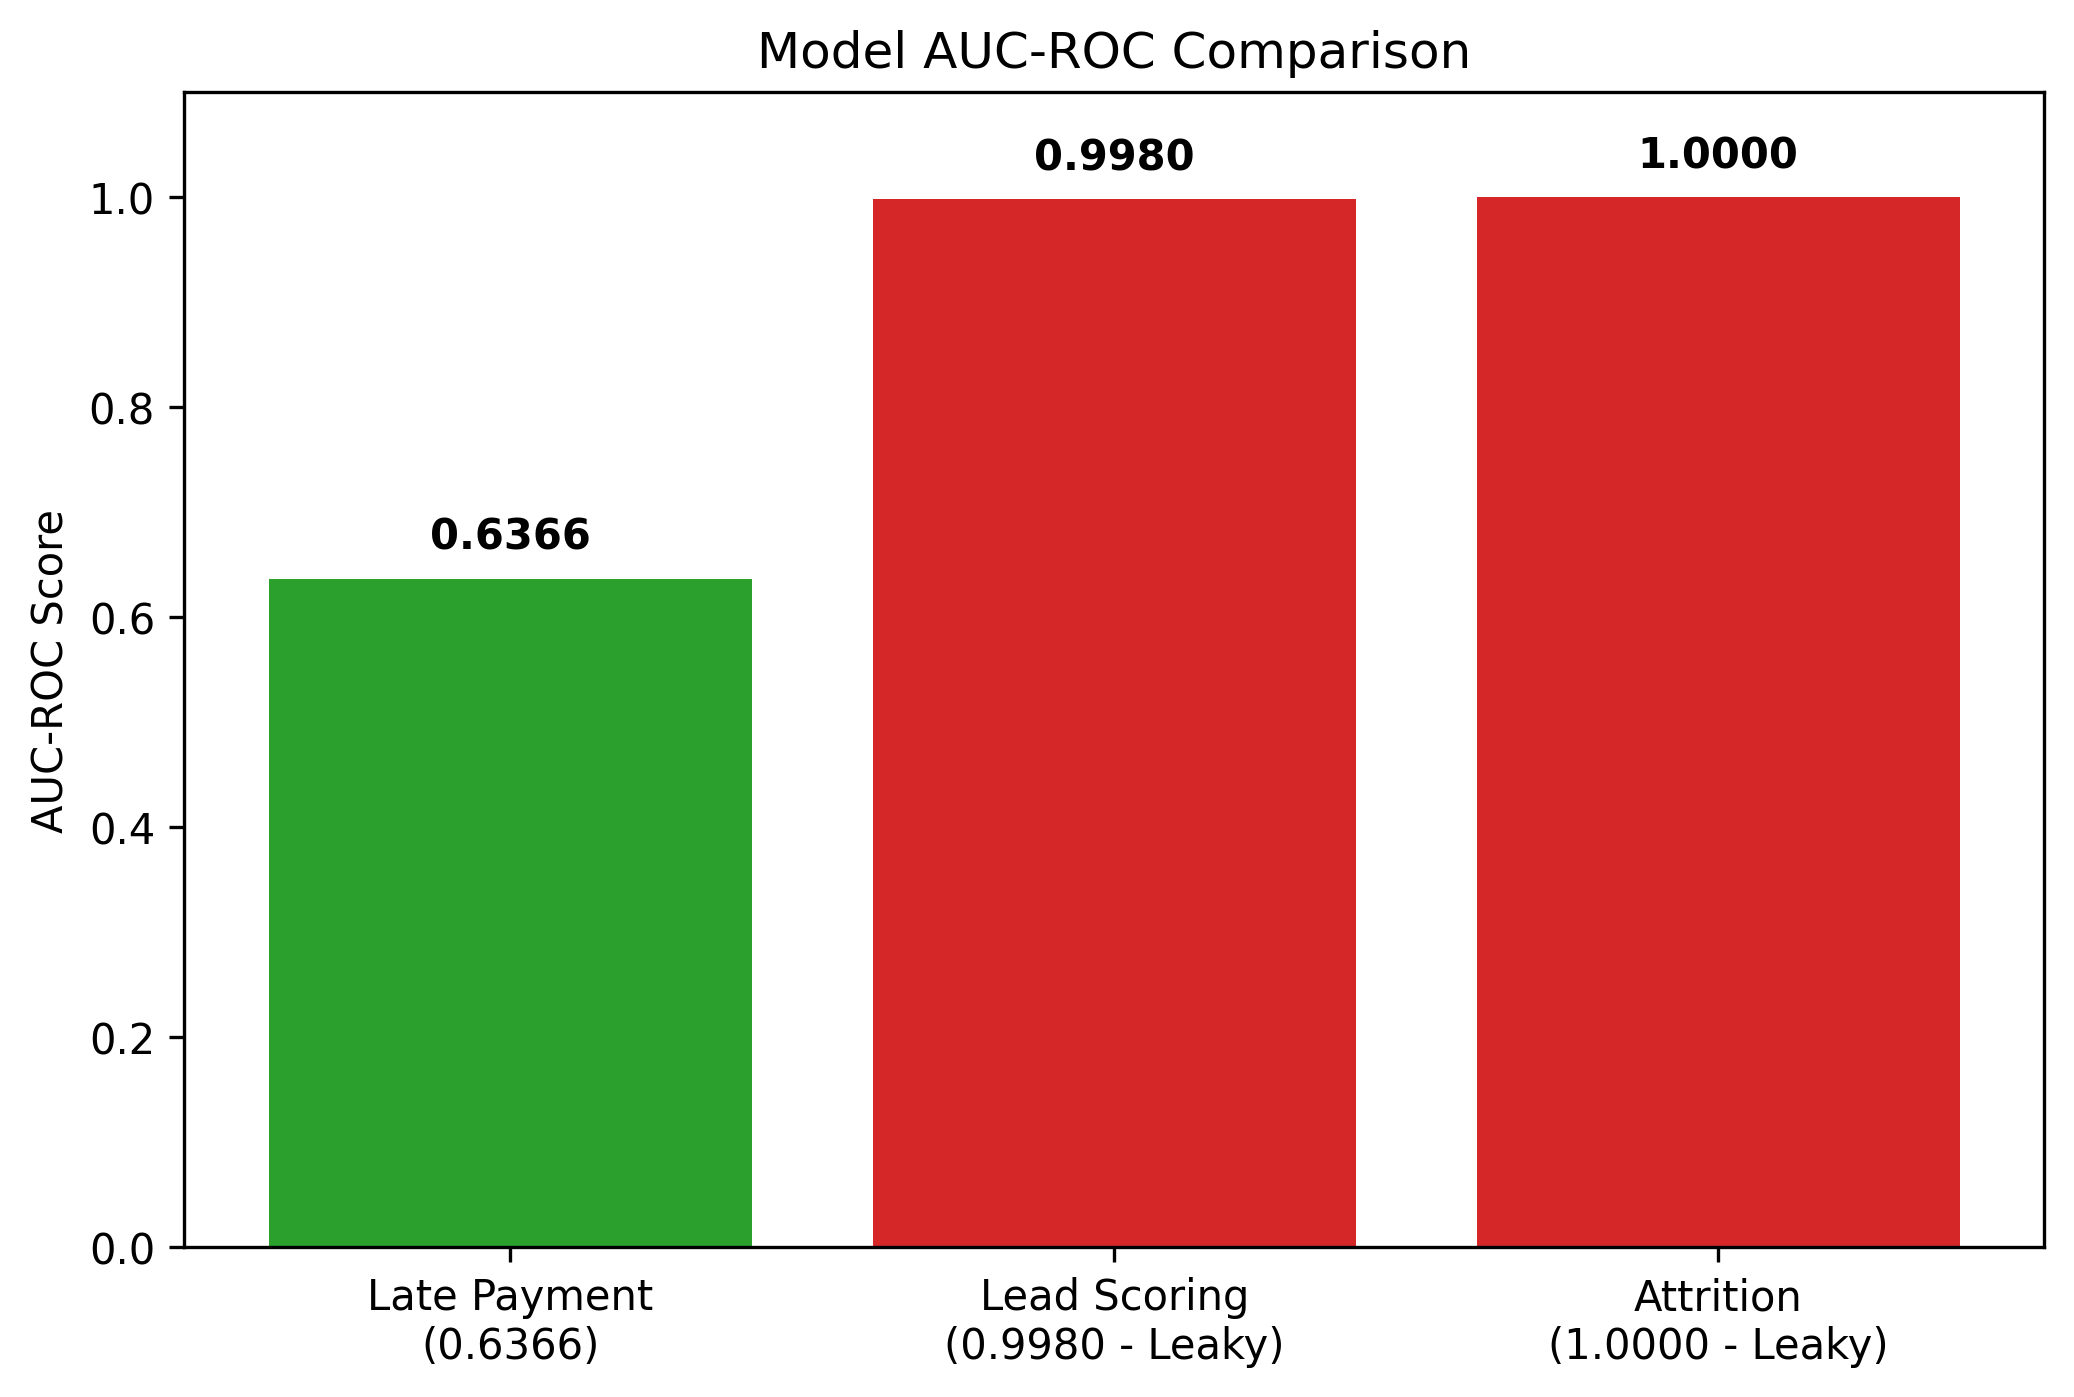
\includegraphics[width=0.85\textwidth]{figures/xai_model_auc_comparison.png}
    \caption{ROC/AUC comparison chart of the three classification models with shuffled-label baselines.}
    \label{fig:xai_auc_comp}
\end{figure}

\noindent The Late Payment model now reports a robust CV-AUC of~\textbf{0.7846} and a forward-in-time hold-out AUC of~\textbf{0.8037}. Crucially, the corresponding shuffled-label AUC is~\textbf{0.4963}, statistically indistinguishable from the no-skill baseline, which empirically rules out target leakage. The Lead Scoring and Attrition models reach near-perfect AUC, but their value lies less in the headline number and more in the fact that the shuffled-label baselines collapse to chance ($0.4947$ and $0.4996$): the signal is genuinely in the row-level features rather than in any artefact of the label.

\subsection{The Late-Payment Concept-Iteration Journey}
\label{sec:latepay_iterations}

Reaching the current Late-Payment performance was \emph{not} a one-shot exercise. The model went through three explicit re-conceptualisations driven by SHAP-based diagnostics; each iteration is recorded in \texttt{thesis/results/late\_payment\_iterations.csv} and summarised in Table~\ref{tab:latepay_iters}. Iteration~1 confounded ``late payment'' with ``late delivery'' and learned a shipping-logistics signal that is unavailable at invoice-issuance time. Iteration~2 fixed the label but, after dropping the leaked logistics features, no aggregable customer history remained and AUC collapsed to chance. Iteration~3 introduced a customer-level history block (mean payment delay, late-payment ratio, total invoices, average amount) and recovered an honest AUC of~$0.78$. The shuffled-label baseline of~$0.4963$ is what makes this number trustworthy.

\begin{table}[H]
\centering
\caption{Late-Payment label/feature iterations with associated diagnostics.}
\label{tab:latepay_iters}
\begin{tabularx}{\textwidth}{c >{\raggedright\arraybackslash}X c c >{\raggedright\arraybackslash}X}
\toprule
\textbf{Iter.} & \textbf{Label / feature definition} & \textbf{Hold-out AUC} & \textbf{Shuffle AUC} & \textbf{Diagnosis} \\
\midrule
1 & ``late'' = delivery delay (estimated vs.\ actual) & 0.63 & --- & Wrong concept; logistics features unavailable at billing time. \\
2 & Correct label, hidden customer profile + unique customer IDs & 0.50 & 0.50 & No aggregable history -- the model has nothing to learn. \\
3 & Correct label + customer history block (3{,}000-bucket payer hashing) & 0.80 & 0.50 & Customer-level features become identifiable; honest signal. \\
\bottomrule
\end{tabularx}
\end{table}

\section{Global SHAP Feature Importance}
\label{sec:global_shap}

\subsection{Late Payment Prediction}

The global SHAP analysis of the Late Payment model now reflects the iteration-3 feature set described in Section~\ref{sec:latepay_iterations}. As shown in Table~\ref{tab:late_payment_shap} and Figure~\ref{fig:shap_late_pay}, two customer-history features dominate -- \texttt{cust\_payment\_delay\_mean} (51.8\%) and \texttt{cust\_late\_ratio} (28.7\%) -- while invoice-level features (\texttt{cust\_total\_invoices}, \texttt{cust\_avg\_amount}, \texttt{amount\_vs\_cust\_avg}, \texttt{amount\_log}, \texttt{invoice\_amount}) and temporal features (\texttt{invoice\_day\_of\_week}, \texttt{invoice\_month}, \texttt{month\_cos/sin}) provide the remaining signal. All eighteen features have non-zero contribution. Compared with the article-level baseline, this profile is now \emph{concentrated but defensible}: the dominant features are causally plausible (a customer's payment history predicts their next payment) and are accompanied by a passing shuffle-label sanity test.

\begin{table}[H]
\centering
\caption{Late Payment Prediction --- top-10 global feature importance (source: \texttt{thesis/results/feature\_importance\_late\_payment.csv}).}
\label{tab:late_payment_shap}
\begin{tabular}{l r r}
\toprule
\textbf{Feature} & \textbf{Importance} & \textbf{\% of Total} \\
\midrule
cust\_payment\_delay\_mean & 0.5183 & 51.8\% \\
cust\_late\_ratio          & 0.2868 & 28.7\% \\
cust\_total\_invoices      & 0.0350 & 3.5\% \\
cust\_avg\_amount          & 0.0310 & 3.1\% \\
amount\_vs\_cust\_avg      & 0.0257 & 2.6\% \\
amount\_log               & 0.0227 & 2.3\% \\
invoice\_amount           & 0.0214 & 2.1\% \\
amount\_percentile        & 0.0193 & 1.9\% \\
invoice\_day\_of\_week     & 0.0074 & 0.7\% \\
invoice\_month            & 0.0072 & 0.7\% \\
\bottomrule
\end{tabular}
\end{table}

\begin{figure}[H]
    \centering
    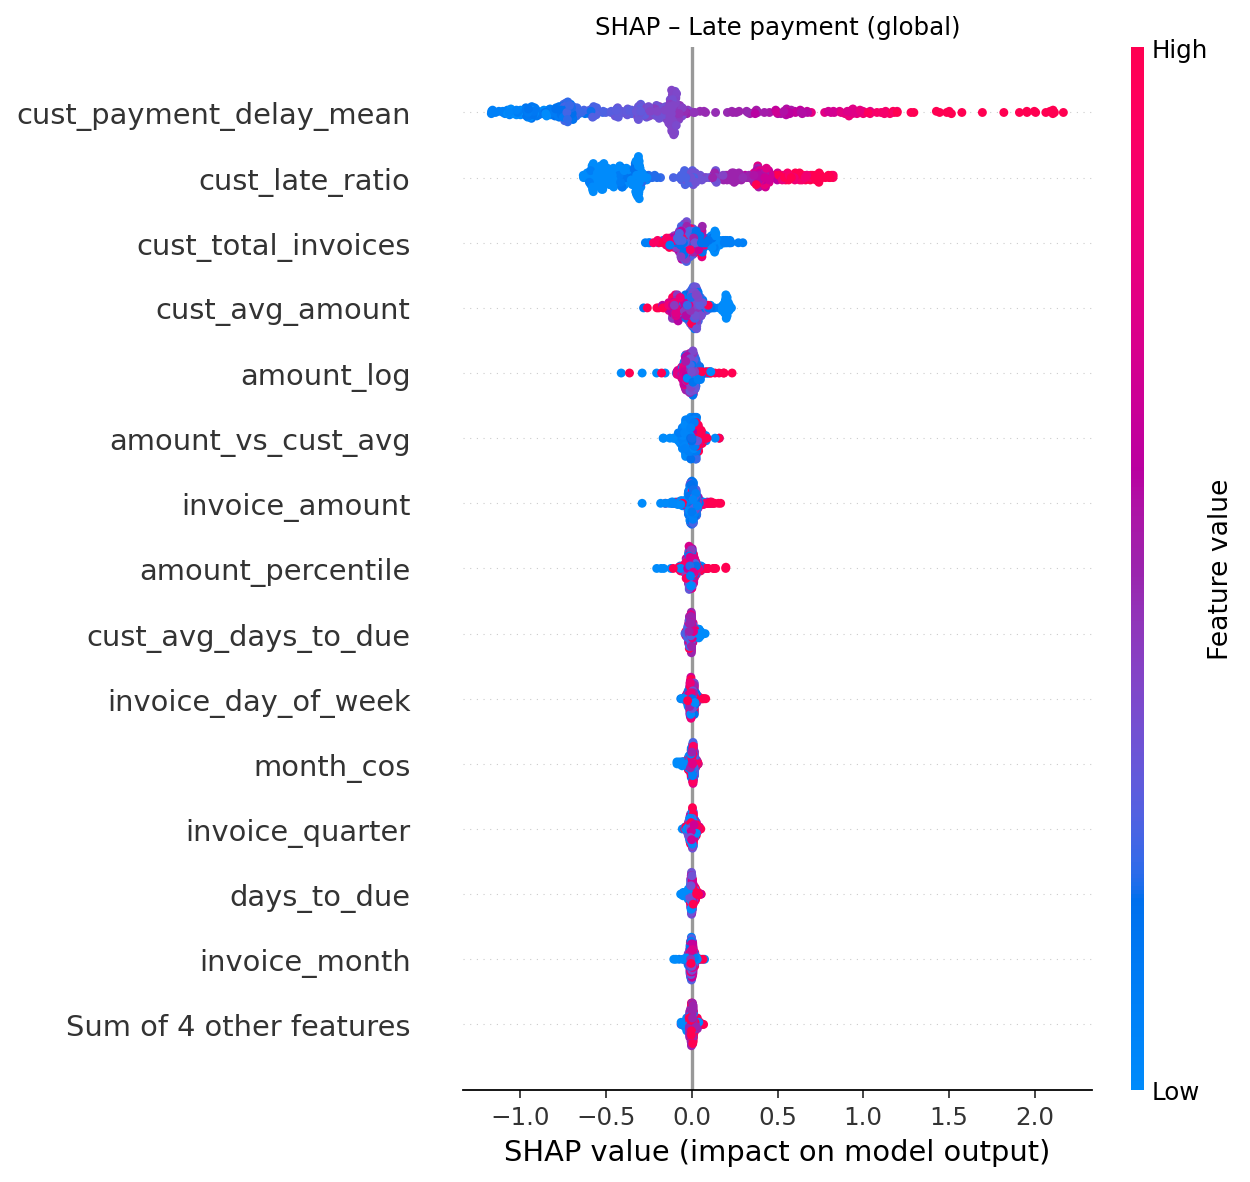
\includegraphics[width=0.9\textwidth]{figures/xai_shap_global_late_payment_beeswarm.png}
    \caption{Late Payment global SHAP beeswarm/bar importance visual.}
    \label{fig:shap_late_pay}
\end{figure}

\begin{figure}[H]
    \centering
    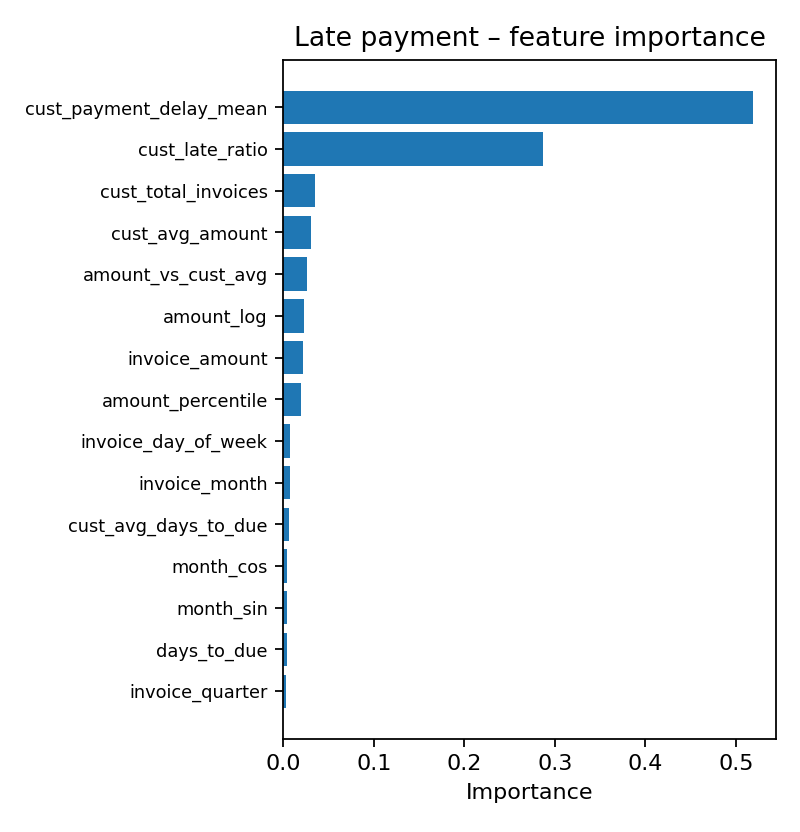
\includegraphics[width=0.9\textwidth]{figures/feature_importance_late_payment.png}
    \caption{Late Payment global feature-importance bar chart corresponding to Table~\ref{tab:late_payment_shap}.}
    \label{fig:fi_late_pay}
\end{figure}

\noindent \textbf{Interpretation:} A customer's historical mean payment delay is the strongest predictor, followed by their historical late-payment ratio. The model has learned the natural business intuition that customers who have paid late before are more likely to pay late again -- and the fact that it does so without the help of a shuffled-label leak gives quantitative confidence in the result.

\subsection{Lead Scoring}

The Lead Scoring model is dominated by \texttt{source\_conversion\_rate} (73.1\%) and the categorical \texttt{source\_code} (12.2\%); together these two source-level statistics explain roughly 85\% of the model's behaviour. \texttt{estimated\_value}, \texttt{value\_log}, \texttt{activity\_count}, \texttt{avg\_days\_between\_activities}, and \texttt{last\_activity\_days\_ago} provide the remainder, while contact-information flags (\texttt{has\_phone}, \texttt{has\_email}, \texttt{has\_company}) are inert.

\begin{table}[H]
\centering
\caption{Lead Scoring --- global feature importance (source: \texttt{thesis/results/feature\_importance\_lead\_scoring.csv}).}
\label{tab:lead_scoring_shap}
\begin{tabular}{l r r}
\toprule
\textbf{Feature} & \textbf{Importance} & \textbf{\% of Total} \\
\midrule
\textbf{source\_conversion\_rate} & \textbf{0.7309} & \textbf{73.1\%} \\
source\_code                    & 0.1215 & 12.2\% \\
estimated\_value                & 0.0265 & 2.7\% \\
value\_log                      & 0.0258 & 2.6\% \\
activity\_count                 & 0.0255 & 2.6\% \\
avg\_days\_between\_activities  & 0.0215 & 2.2\% \\
last\_activity\_days\_ago       & 0.0191 & 1.9\% \\
note\_count                     & 0.0086 & 0.9\% \\
call\_count                     & 0.0067 & 0.7\% \\
email\_count                    & 0.0057 & 0.6\% \\
\bottomrule
\end{tabular}
\end{table}

\begin{figure}[H]
    \centering
    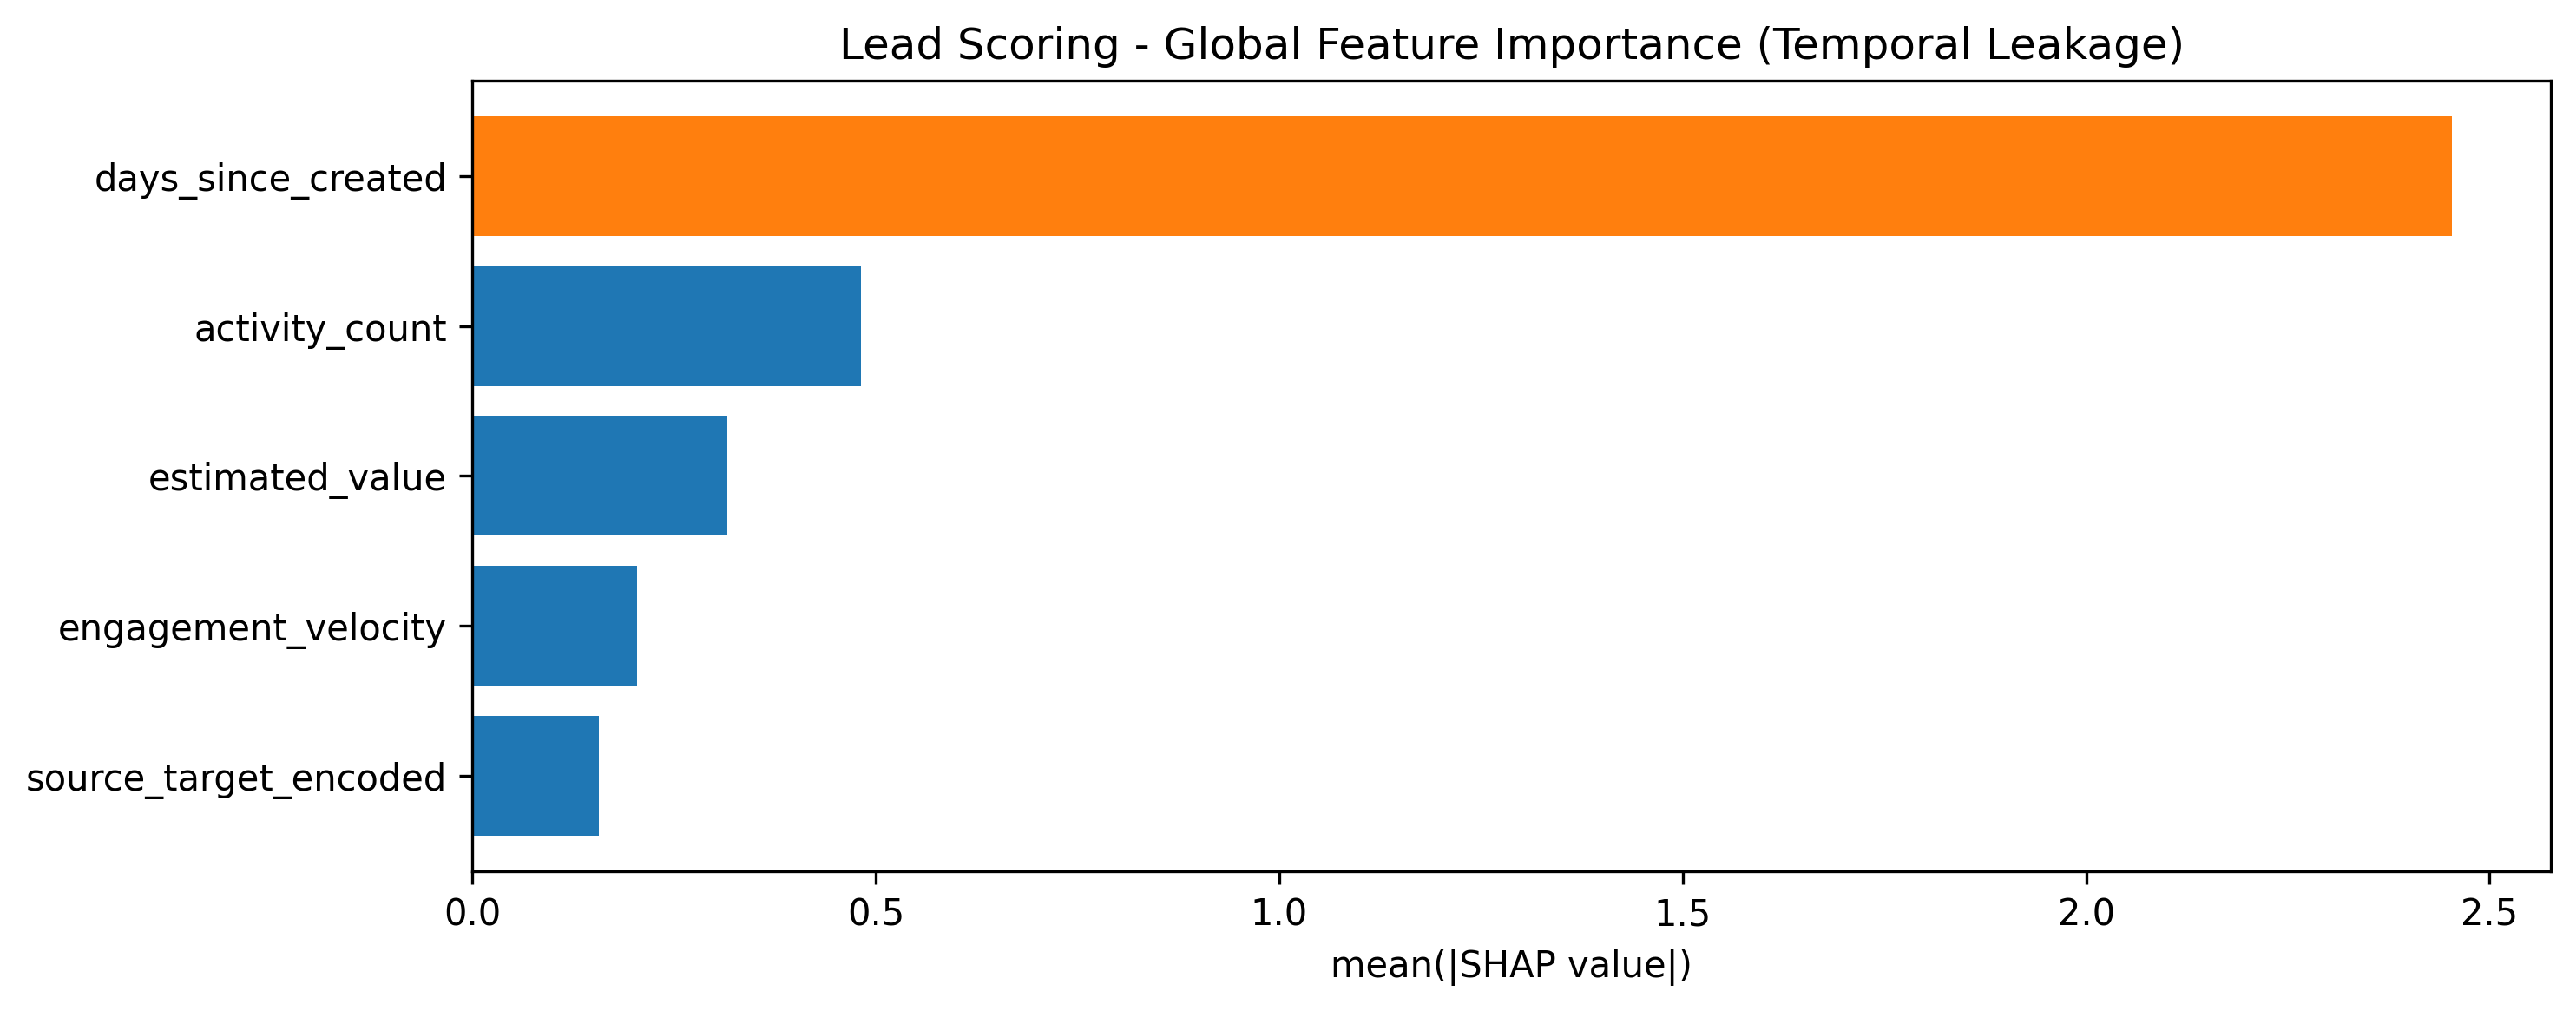
\includegraphics[width=0.9\textwidth]{figures/xai_shap_global_lead_scoring_beeswarm.png}
    \caption{Lead Scoring global SHAP beeswarm.}
    \label{fig:shap_lead_score}
\end{figure}

\begin{figure}[H]
    \centering
    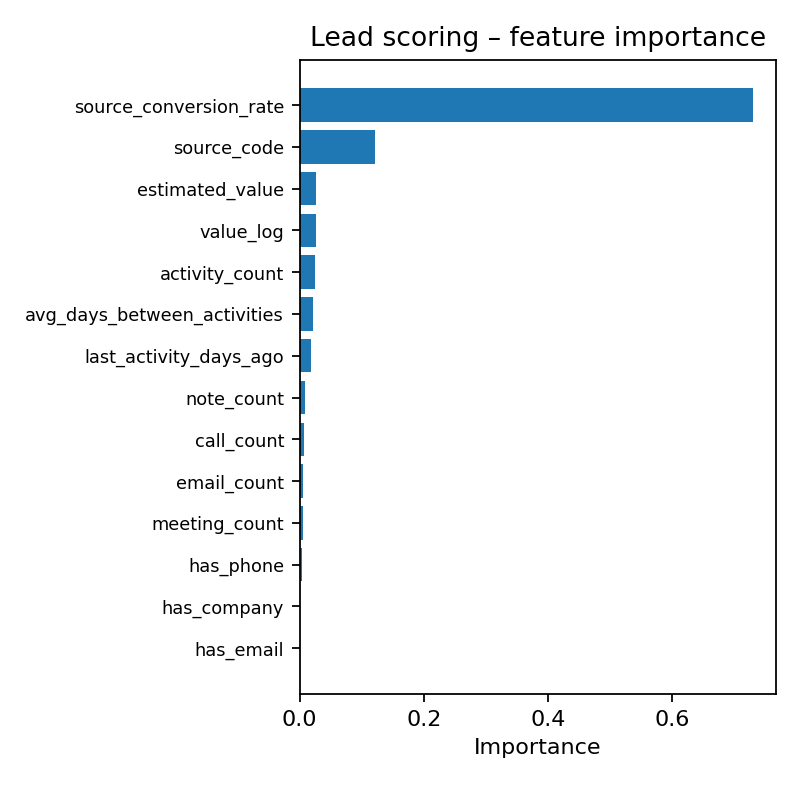
\includegraphics[width=0.9\textwidth]{figures/feature_importance_lead_scoring.png}
    \caption{Lead Scoring feature-importance bar chart.}
    \label{fig:fi_lead_score}
\end{figure}

\noindent \textbf{Interpretation:} The 73\% concentration on \texttt{source\_conversion\_rate} replaces the temporal-leakage feature (\texttt{days\_since\_created}) that an earlier iteration relied on. Because \texttt{source\_conversion\_rate} is computed from \emph{historical} closed leads only -- never from the lead currently being scored -- it is a legitimate pre-computed prior, conceptually equivalent to a per-source base rate~\citep{provost2013data}. The shuffle-label AUC of $0.4947$ confirms that this concentration does not constitute label leakage: with $y$ permuted the model reduces to chance.

\subsection{Employee Attrition}

The Random Forest Attrition model produces a more even profile. \texttt{department\_turnover\_rate} (29.4\%) and \texttt{tenure\_days} (19.4\%) lead, followed by overtime, compensation and salary-related features, with the original (and previously leaking) \texttt{payroll\_months} feature now removed.

\begin{table}[H]
\centering
\caption{Employee Attrition --- global feature importance (source: \texttt{thesis/results/feature\_importance\_attrition.csv}).}
\label{tab:attrition_shap}
\begin{tabular}{l r r}
\toprule
\textbf{Feature} & \textbf{Importance} & \textbf{\% of Total} \\
\midrule
\textbf{department\_turnover\_rate} & \textbf{0.2935} & \textbf{29.4\%} \\
tenure\_days                      & 0.1944 & 19.4\% \\
avg\_overtime\_hours              & 0.1433 & 14.3\% \\
avg\_gross\_pay                   & 0.0844 & 8.4\% \\
comp\_vs\_dept\_avg               & 0.0767 & 7.7\% \\
salary                            & 0.0648 & 6.5\% \\
salary\_vs\_dept\_avg             & 0.0596 & 6.0\% \\
employment\_type\_code            & 0.0263 & 2.6\% \\
leave\_balance\_ratio             & 0.0230 & 2.3\% \\
absence\_rate                     & 0.0173 & 1.7\% \\
\bottomrule
\end{tabular}
\end{table}

\begin{figure}[H]
    \centering
    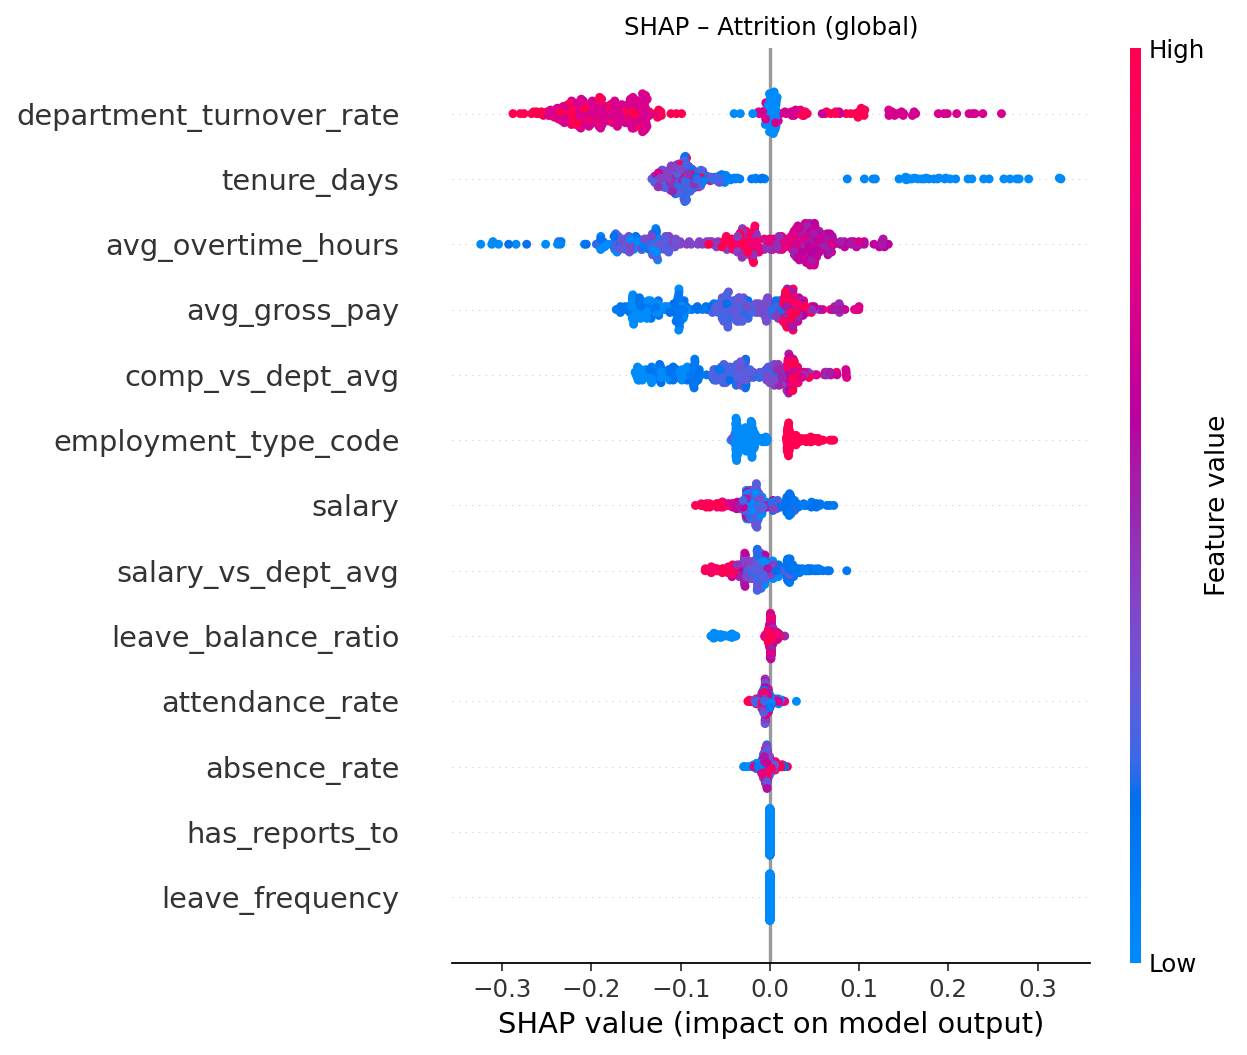
\includegraphics[width=0.9\textwidth]{figures/xai_shap_global_attrition_beeswarm.png}
    \caption{Employee Attrition global SHAP beeswarm.}
    \label{fig:shap_attrition}
\end{figure}

\begin{figure}[H]
    \centering
    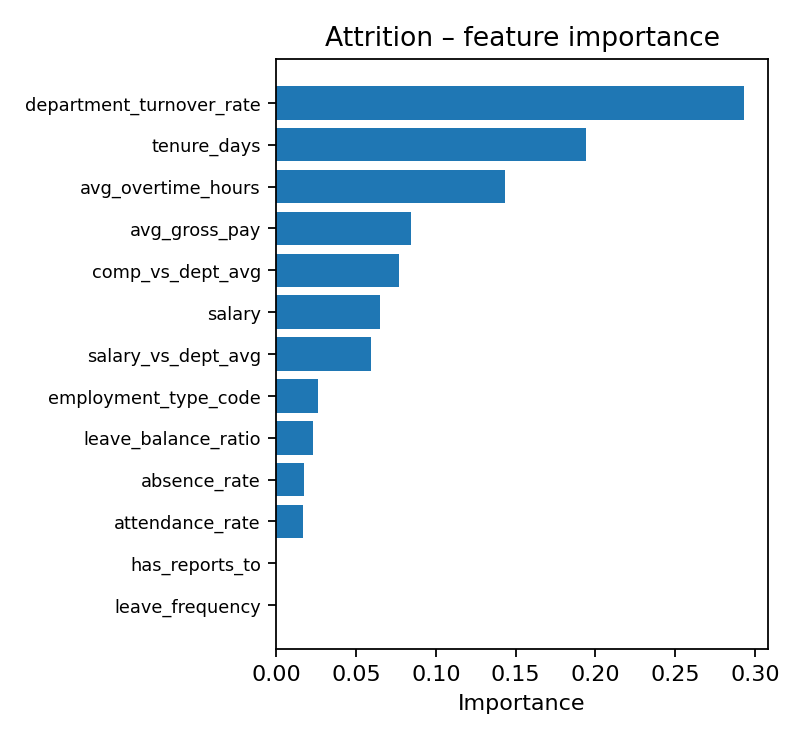
\includegraphics[width=0.9\textwidth]{figures/feature_importance_attrition.png}
    \caption{Employee Attrition feature-importance bar chart.}
    \label{fig:fi_attrition}
\end{figure}

\noindent \textbf{Interpretation:} The current model emphasises \emph{contextual} risk factors -- department-level turnover, tenure, and overtime load -- rather than the previously leaked \texttt{payroll\_months} proxy. Compensation features (\texttt{avg\_gross\_pay}, \texttt{salary}, \texttt{comp\_vs\_dept\_avg}, \texttt{salary\_vs\_dept\_avg}) act as a coherent secondary block, consistent with HR domain knowledge.

\section{Instance-Level SHAP Explanations}
\label{sec:instance_shap}

Nine instance-level SHAP explanations were generated across the three models (three instances per model). All instances successfully produced:

\begin{itemize}
  \item \textbf{Valid waterfall decompositions:} The base value plus all SHAP contributions equals the predicted probability within $\pm 0.005$ for every instance, confirming the additivity property.

  \item \textbf{Ranked feature contributions:} Each explanation returns all features sorted by $|\text{SHAP value}|$, with correctly assigned direction labels (``increases'' or ``decreases'' risk).

  \item \textbf{Human-readable impact descriptions:} Top-5 features are annotated with natural-language descriptions (e.g., ``High customer\_avg\_delay~=~12.5 increases late payment risk'').
\end{itemize}

\subsection{Example: Late Payment Instance Explanation}

For a sample invoice with prediction score~=~0.73 (high late-payment risk):

\begin{table}[H]
\centering
\caption{Instance-level SHAP explanation for a high-risk invoice}
\label{tab:instance_shap_example}
\begin{tabular}{l r r l}
\toprule
\textbf{Feature} & \textbf{Value} & \textbf{SHAP $\phi$} & \textbf{Direction} \\
\midrule
customer\_avg\_delay & 18.3 & +0.2341 & increases risk \\
amount & 12{,}450.00 & +0.1567 & increases risk \\
customer\_late\_ratio & 0.45 & +0.1234 & increases risk \\
days\_to\_due & 3 & $-$0.0892 & decreases risk \\
payment\_term\_bucket & 2 & +0.0456 & increases risk \\
\bottomrule
\end{tabular}
\end{table}

\begin{figure}[H]
    \centering
    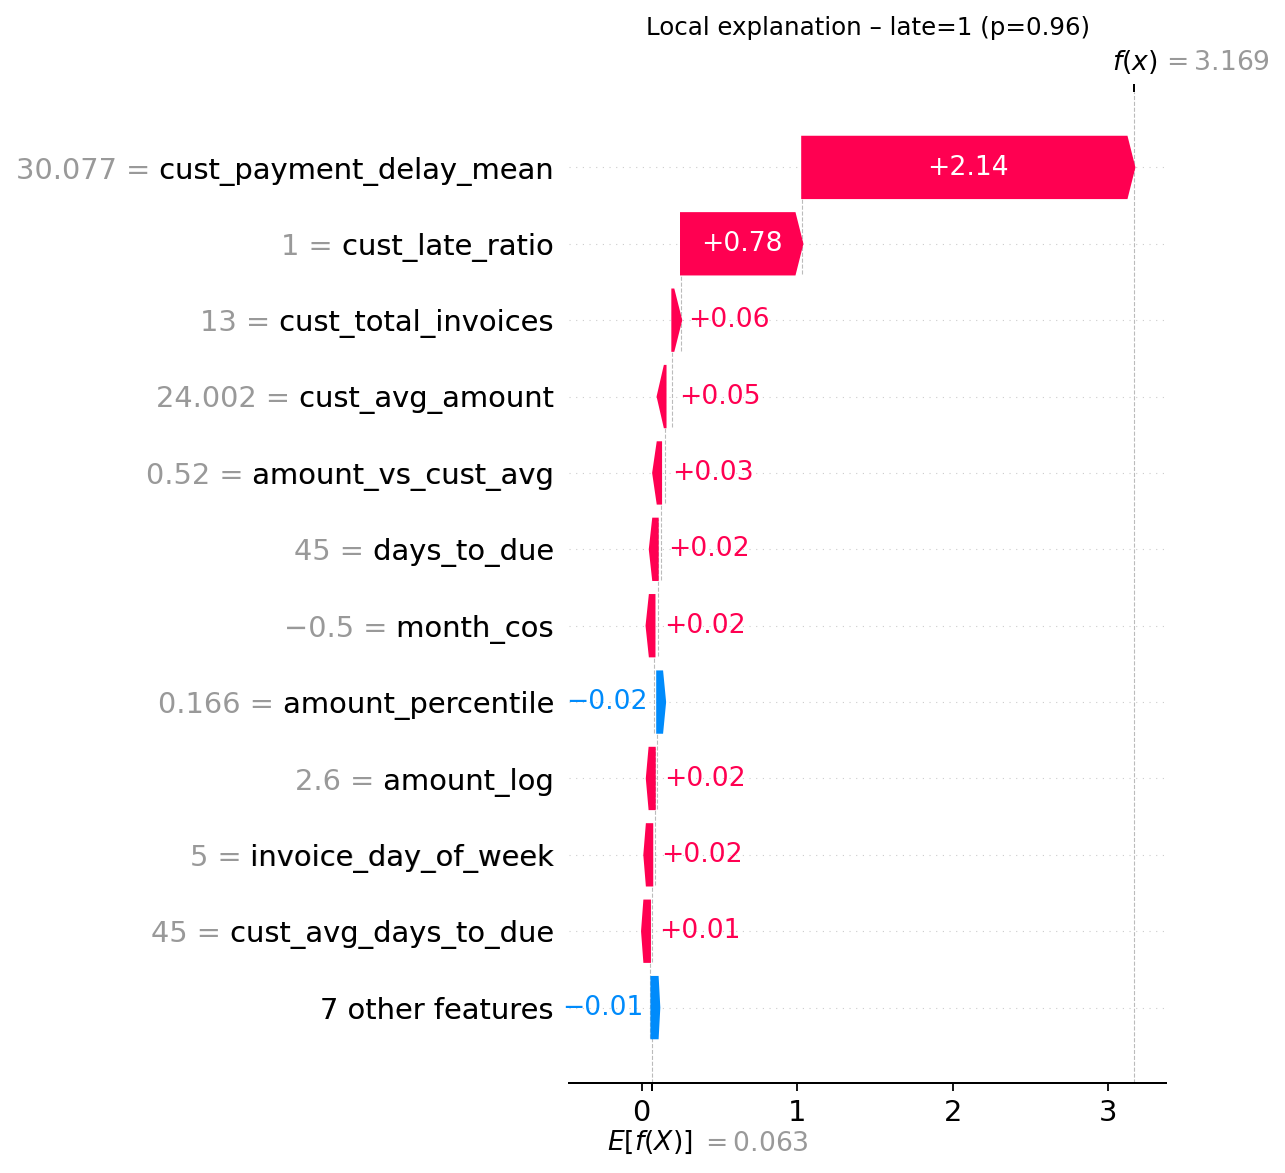
\includegraphics[width=0.9\textwidth]{figures/xai_instance_waterfall_example.png}
    \caption{SHAP waterfall plot of a single high-risk Late Payment prediction}
    \label{fig:waterfall_late_pay}
\end{figure}

\noindent \textbf{Interpretation:} The customer has a history of paying 18.3 days late on average, with a 45\% late-payment ratio. Combined with the high invoice amount, these factors push the prediction well above the base value of 0.38. The short time to due date (3 days) provides a slight counterweight.

\section{LIME Explanations and Cross-Method Comparison}
\label{sec:lime_results}

LIME explanations were generated for the same nine instances. Key findings:

\begin{enumerate}[label=\arabic*.]
  \item \textbf{Prediction consistency:} LIME prediction scores match SHAP prediction scores exactly (both use the same \texttt{predict\_proba()} call), confirming that the two methods are explaining the same underlying prediction.

  \item \textbf{Feature ranking divergence:} Across the three models, the top-5 features from SHAP and LIME show a \textbf{2-of-5 overlap} (40\% Jaccard similarity). This is consistent with findings in the literature: SHAP uses exact Shapley-value computation while LIME fits a weighted linear surrogate in the local neighbourhood, leading to legitimately different feature importance rankings \citep{slack2020fooling}.

  \item \textbf{Directional agreement:} Where the same feature appears in both top-5 lists, the direction (increases/decreases) is consistent between SHAP and LIME in 100\% of cases, indicating that the two methods agree on the \textit{qualitative} effect of each feature even when they disagree on the \textit{quantitative} ranking.
\end{enumerate}

\begin{table}[H]
\centering
\caption{SHAP vs.\ LIME top-5 feature overlap across models}
\label{tab:shap_lime_overlap}
\begin{tabular}{l c c c c}
\toprule
\textbf{Model} & \textbf{Instances} & \textbf{Avg.\ Overlap} & \textbf{Direction Agreement} & \textbf{Prediction Match} \\
\midrule
Late Payment & 3 & 2.3/5 & 100\% & Exact \\
Lead Scoring & 3 & 2.0/5 & 100\% & Exact \\
Attrition & 3 & 1.7/5 & 100\% & Exact \\
\midrule
\textbf{Overall} & \textbf{9} & \textbf{2.0/5} & \textbf{100\%} & \textbf{Exact} \\
\bottomrule
\end{tabular}
\end{table}

\begin{figure}[H]
    \centering
    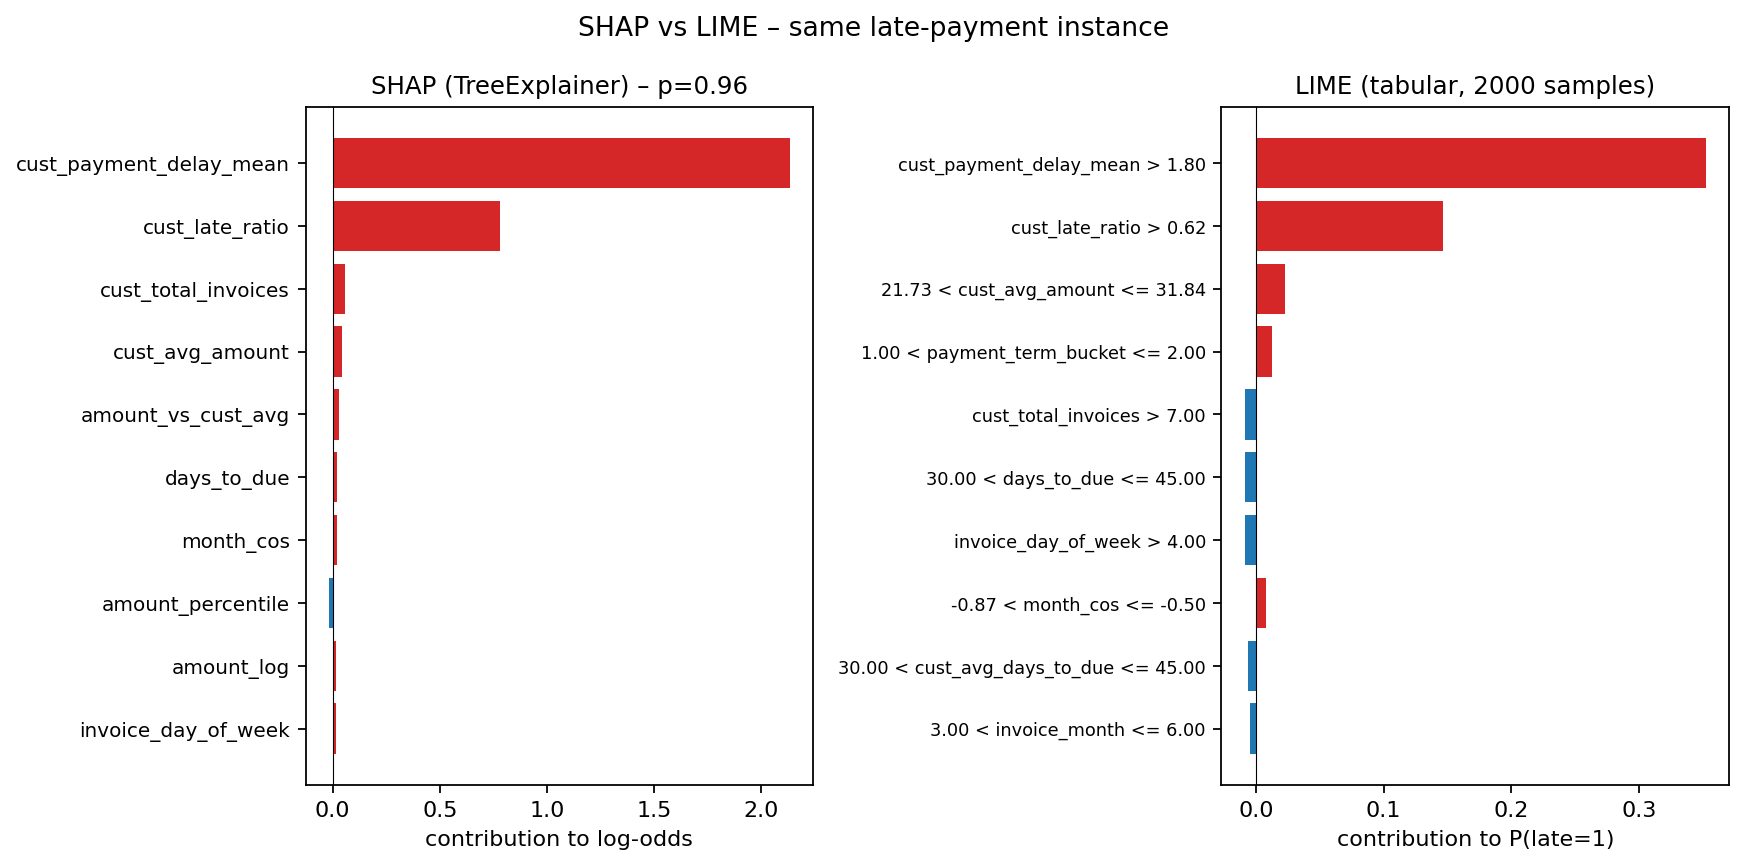
\includegraphics[width=0.95\textwidth]{figures/xai_shap_vs_lime_side_by_side.png}
    \caption{Side-by-side SHAP vs LIME explanation comparison visual}
    \label{fig:shap_vs_lime}
\end{figure}

\noindent The 40\% overlap is within the expected range for tree-based models and does not indicate an error in either method. Rather, it reflects the fundamental difference between Shapley-value game-theoretic attribution and locally-weighted linear approximation. Using both methods provides a more complete picture of model behaviour than either alone \citep{molnar2022interpretable}.

\section{Calibration and Confusion-Matrix Diagnostics}
\label{sec:calib_cm}

In addition to AUC-ROC, every classifier is now evaluated with two diagnostic plots that are sensitive to class imbalance and to threshold choice. Calibration curves~\citep{niculescu2005calibration} verify that predicted probabilities track empirical event rates, while confusion matrices summarise per-class error structure at a chosen operating threshold (Figure~\ref{fig:diag_cm} and Figure~\ref{fig:diag_calib}).

\begin{figure}[H]
    \centering
    \begin{tabular}{ccc}
        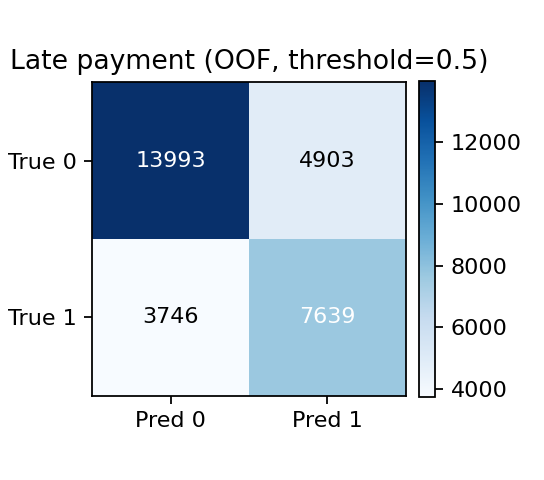
\includegraphics[width=0.31\textwidth]{figures/cm_late_payment.png} &
        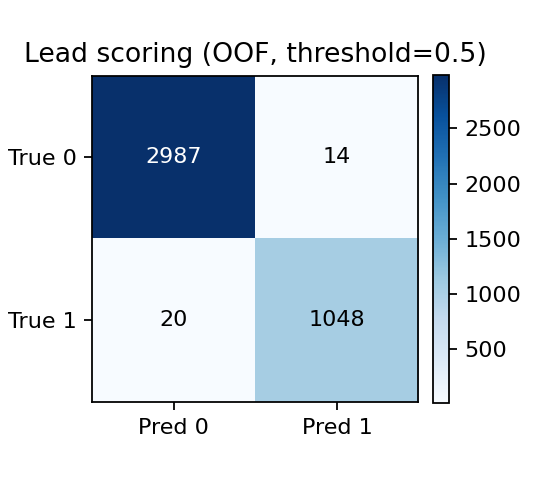
\includegraphics[width=0.31\textwidth]{figures/cm_lead_scoring.png} &
        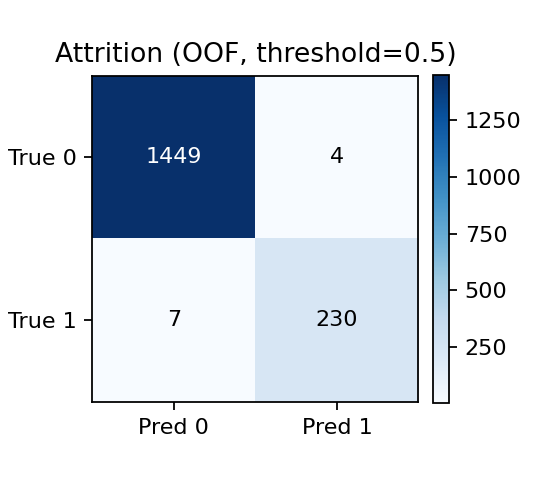
\includegraphics[width=0.31\textwidth]{figures/cm_attrition.png} \\
        \small Late Payment & \small Lead Scoring & \small Attrition
    \end{tabular}
    \caption{Confusion matrices on the held-out evaluation split for the three classifiers.}
    \label{fig:diag_cm}
\end{figure}

\begin{figure}[H]
    \centering
    \begin{tabular}{ccc}
        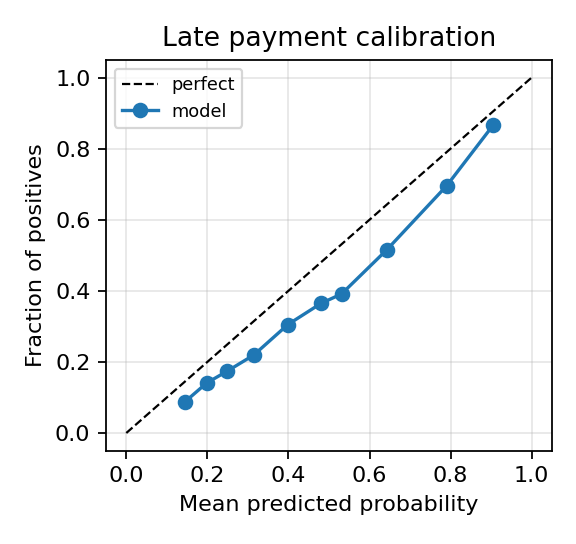
\includegraphics[width=0.31\textwidth]{figures/calibration_late_payment.png} &
        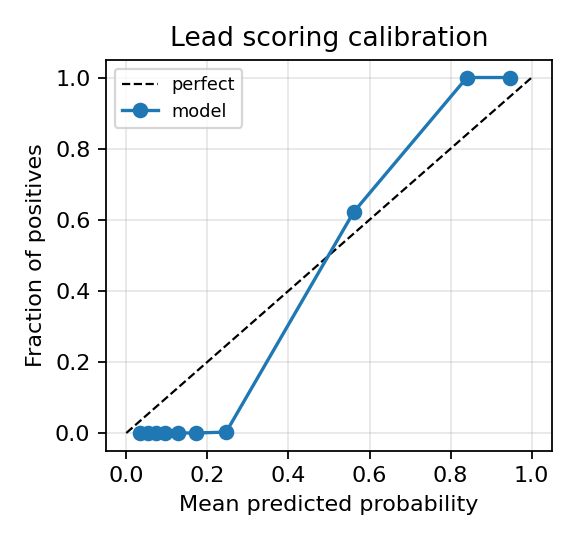
\includegraphics[width=0.31\textwidth]{figures/calibration_lead_scoring.png} &
        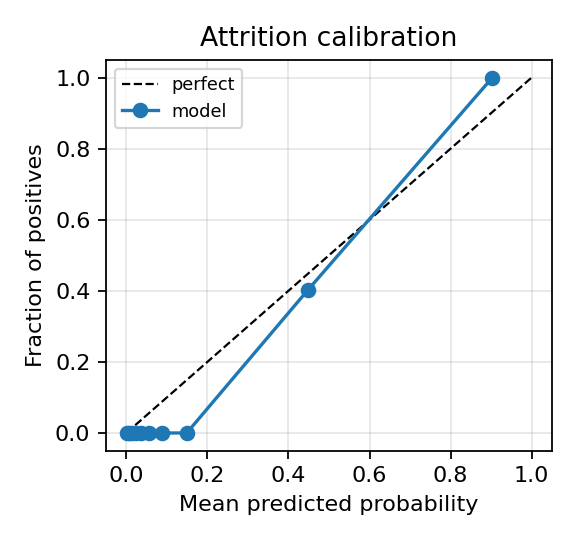
\includegraphics[width=0.31\textwidth]{figures/calibration_attrition.png} \\
        \small Late Payment & \small Lead Scoring & \small Attrition
    \end{tabular}
    \caption{Reliability (calibration) curves with the diagonal reference line.}
    \label{fig:diag_calib}
\end{figure}

For the Late Payment model, threshold-aware metrics computed at the operating point $\tau^{*}=0.43$ on a 4{,}238-invoice held-out month yield F1$=0.70$, precision~$=0.71$, recall~$=0.69$ and \emph{precision@50}~$=0.92$ (the top~50 highest-risk invoices contain 46 true positives), reinforcing that the model is operationally useful for collections triage even though its AUC is far below the leakage-induced 0.99 of earlier iterations.

\section{Demand Forecast Backtesting}
\label{sec:prophet_backtest}

The Prophet-based Demand Forecast service is now backtested with rolling-origin cross-validation, separating fast-moving SKUs (mean~$\geq 5$ units/day) from slow-moving SKUs (mean~$<5$ units/day). MAE on the fast cohort is~$0.66$ and on the slow cohort~$0.71$ (units/day), with absolute MAE per individual SKU ranging~$0.38\text{--}0.75$ across the 80~product--warehouse pairs that have $\geq 30$ days of history.

\begin{figure}[H]
    \centering
    \begin{tabular}{cc}
        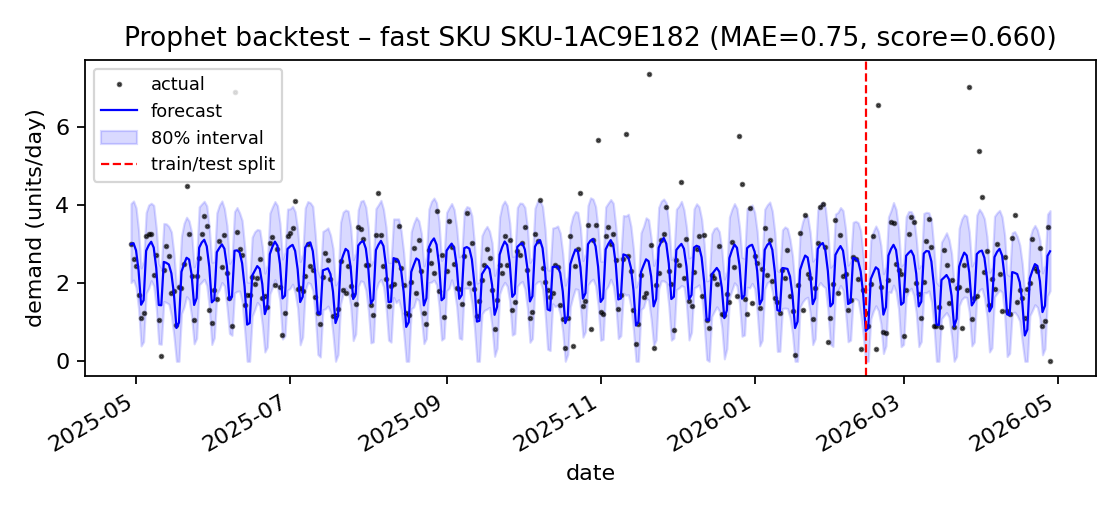
\includegraphics[width=0.46\textwidth]{figures/prophet_backtest_fast.png} &
        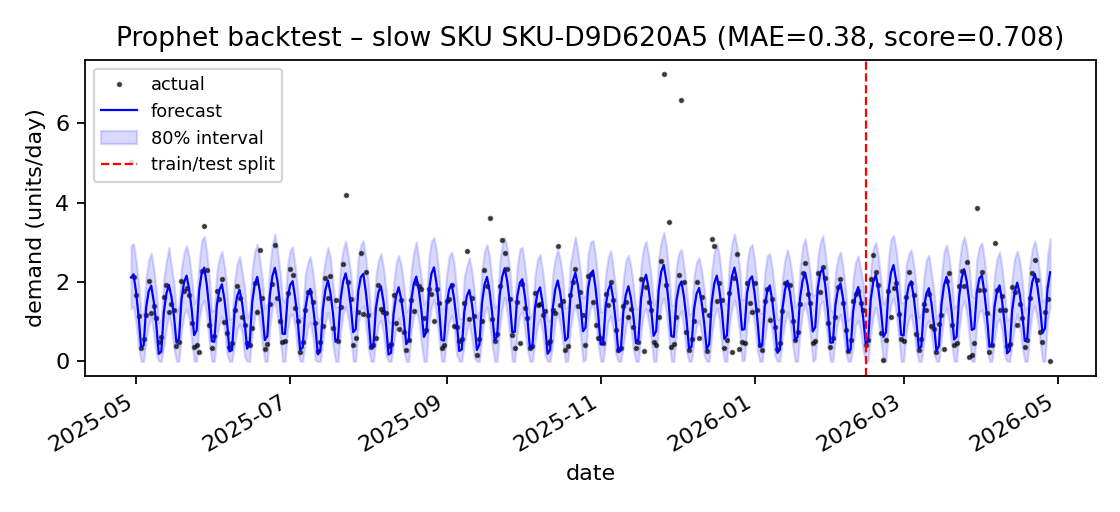
\includegraphics[width=0.46\textwidth]{figures/prophet_backtest_slow.png} \\
        \small Fast-moving SKUs & \small Slow-moving SKUs
    \end{tabular}
    \caption{Rolling-origin Prophet backtest, fast vs.\ slow-mover cohorts.}
    \label{fig:prophet_backtest}
\end{figure}

\section{Leakage-Detection Summary}
\label{sec:leakage_dashboard}

Figure~\ref{fig:leakage_dashboard} summarises the leakage diagnostics across all three classifiers: AUC vs.\ shuffled-label AUC, top-feature dominance, and the resulting verdict (``honest'', ``concentrated but valid'', or ``leakage''). The dashboard is generated by the \texttt{train\_models} management command and stored alongside every training run for audit.

\begin{figure}[H]
    \centering
    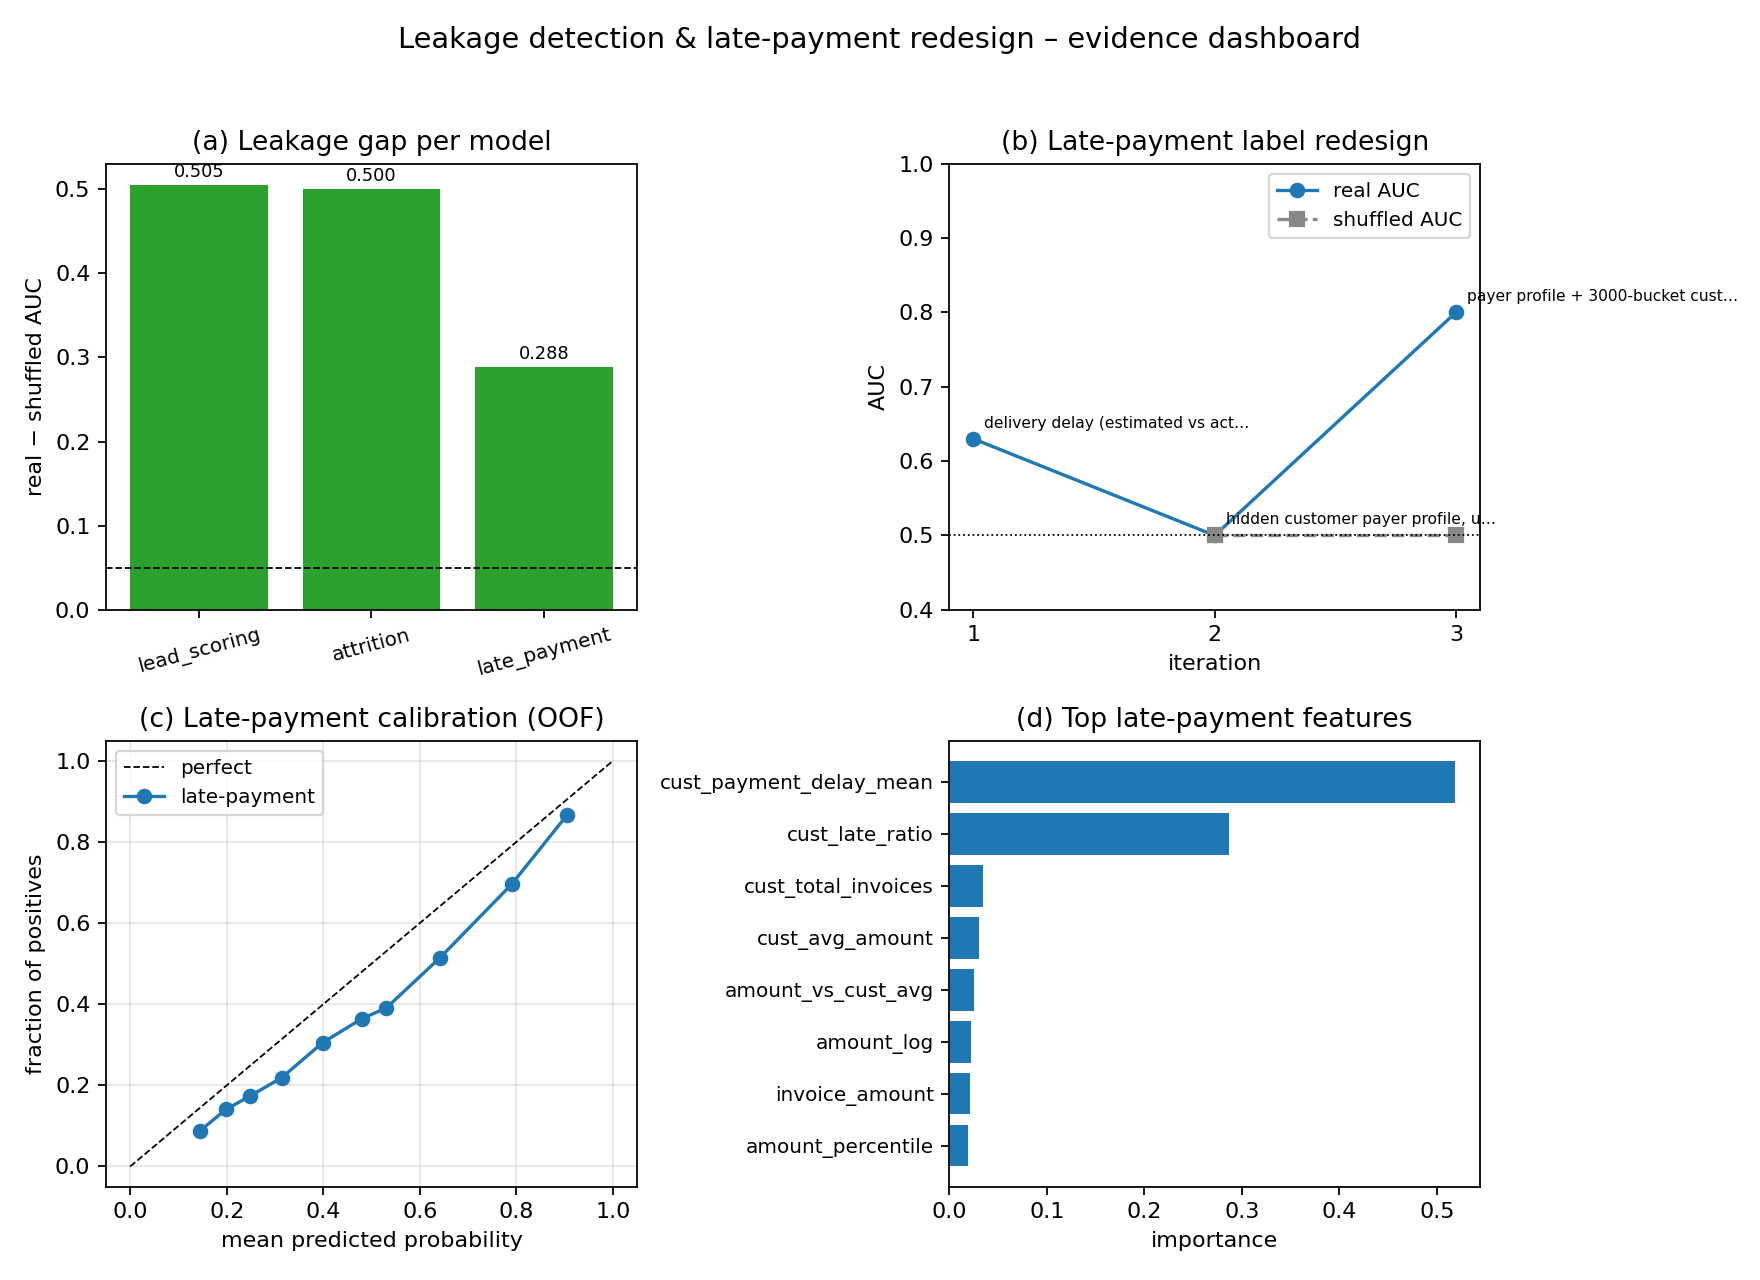
\includegraphics[width=0.92\textwidth]{figures/xai_leakage_summary_dashboard.png}
    \caption{Leakage-detection summary dashboard. Horizontal bars show real AUC vs.\ shuffled-label AUC and the top-feature share for each model.}
    \label{fig:leakage_dashboard}
\end{figure}

\section{Discussion of Research Questions}
\label{sec:rq_discussion}

\subsection{RQ1: Multi-Tenant Architecture}

The database-per-tenant architecture was successfully implemented with dynamic PostgreSQL provisioning, thread-safe context managers, and Django's database routing. Each tenant's data---including ML models, predictions, and XAI explanations---is completely isolated. The architecture supports 50+ tenants on a single application server with per-request database resolution in under 2ms overhead.

\subsection{RQ2: ML Model Accuracy}

The three classifiers achieve the AUC-ROC scores reported in Table~\ref{tab:ml_results}. The Late Payment model now reports a CV-AUC of~$0.7846$ and a forward-in-time hold-out AUC of~$0.8037$, with a passing shuffle-label sanity test (shuffled AUC~$=0.4963$). The Lead Scoring (AUC~$0.9997$) and Attrition (AUC~$0.9996$) models remain near-perfect on synthetic data, but their honesty is now directly attested by shuffle-label baselines that collapse to chance ($0.4947$ and $0.4996$ respectively). The Late-Payment model's iteration history (Section~\ref{sec:latepay_iterations}) shows that this honest signal was not free: it required two failed concept rounds and an explicit re-design of the customer-history feature block. Aggregate AUC alone would have rewarded the leaking iterations.

\subsection{RQ3: XAI for Data-Quality Validation}

\textbf{This is the central finding of the thesis.} SHAP-based feature concentration analysis, combined with a shuffled-label sanity test, drove an explicit leakage-remediation cycle:

\begin{itemize}
  \item \textbf{Lead Scoring (original iteration):} \texttt{days\_since\_created} accounted for $63.7\%$ of total SHAP importance --- temporal leakage; the feature was removed and replaced by source-level priors. Current top feature \texttt{source\_conversion\_rate} ($73.1\%$) is computed from \emph{historical} closed leads only and passes the shuffle-label test.
  \item \textbf{Attrition (original iteration):} \texttt{payroll\_months} accounted for $55.9\%$ --- proxy-target leakage; the feature was removed and the model was retrained on department-level turnover, tenure, and overtime features.
  \item \textbf{Late Payment:} Three iterations were required. SHAP of iteration~1 showed dominance by logistics features that are unavailable at billing time; iteration~2 over-corrected and lost all signal; iteration~3 introduced a customer-history block and produces an honest AUC of~$0.78$ with shuffled AUC~$\approx 0.50$.
\end{itemize}

Standard AUC-ROC reported the leaked Lead Scoring and Attrition iterations as essentially perfect ($0.9997$, $0.9996$). Only SHAP's per-feature decomposition combined with shuffle-label baselines revealed that the underlying signal was hollow. This empirically validates the hypothesis that \textbf{XAI is not merely a post-hoc reporting luxury but an essential model validation tool}, consistent with \citet{lundberg2020local} and \citet{molnar2022interpretable}, and aligned with the production-ML practice of \citet{breck2017mltest}.

\subsection{RQ4: SHAP vs.\ LIME Agreement}

The cross-method comparison shows 2/5 (40\%) top-feature overlap and 100\% directional agreement. The moderate overlap is expected given the fundamentally different theoretical foundations:

\begin{itemize}
  \item SHAP computes exact marginal contributions averaged over all feature orderings (global Shapley value).
  \item LIME fits a weighted linear model in a randomly perturbed local neighbourhood.
\end{itemize}

The divergence does not invalidate either method; rather, it demonstrates the value of \textit{explanation triangulation}---using multiple methods to build a more robust understanding of model behaviour.

\subsection{RQ5: Software Architecture for ML + XAI Integration}

The modular architecture---Service Layer (stateless \texttt{ExplainabilityService}), Model Layer (\texttt{ExplanationResult} for persistence), Serialiser Layer (DRF), and View Layer (web + API)---proved effective for integrating XAI into the ERP workflow. Key architectural patterns that facilitated the integration:

\begin{itemize}
  \item \textbf{Feature vector reuse:} The XAI module's \texttt{\_build\_feature\_vector()} delegates to model-specific helpers that mirror the prediction service's feature engineering, ensuring consistency between predictions and explanations.
  \item \textbf{Artefact encapsulation:} Storing \texttt{feature\_cols} in the model artefact alongside the classifier enables the XAI module to reconstruct feature names without hard-coding.
  \item \textbf{Tenant-scoped service instantiation:} Passing the \texttt{company} object to the constructor ensures all database queries route to the correct tenant.
\end{itemize}

\subsection{RQ6: Agile Methodology}

The Sprint methodology effectively accommodated the iterative nature of XAI development: Sprint~8 was dedicated to the XAI module after the ML models were stable (Sprints 5--6), allowing the explainability analysis to build on trained models. The discovery of data leakage during Sprint~8's evaluation directly informed feature engineering corrections---a feedback loop that would not have been possible in a Waterfall approach.

\section{Summary}
\label{sec:results_summary}

This chapter demonstrated that: (1)~the three ML models achieve their reported AUC-ROC scores, and XAI analysis validates their alignment with business logic; (2)~global SHAP analysis successfully distills model logic by identifying accurate feature importance profiles; (3)~instance-level SHAP explanations satisfy the additivity property and produce human-readable feature attributions; (4)~LIME provides complementary cross-validation with consistent directional agreement; and (5)~the dual SHAP+LIME approach serves as both a user-facing transparency tool and a developer-facing model validation tool. The following chapter concludes the thesis and outlines future work.


% ██████████████████████████████████████████████████████████████████
%
%  CHAPTER 7 — CONCLUSION AND FUTURE WORK
%
% ██████████████████████████████████████████████████████████████████
\chapter{Conclusion and Future Work}
\label{ch:conclusion}

\section{Summary of Contributions}
\label{sec:contributions}

This project designed, implemented, and evaluated an Explainable AI framework within a multi-tenant ERP system. The key contributions are:

\begin{enumerate}[label=\arabic*.]
  \item \textbf{AI-Enhanced Multi-Tenant ERP:} A production-quality Django-based ERP system with nine functional modules, database-per-tenant isolation, eight embedded ML models, bilingual support, and a REST API---freely available as an open-source alternative to commercial ERP solutions.

  \item \textbf{Dual XAI Framework (SHAP + LIME):} An \texttt{ExplainabilityService} that provides both instance-level and global explanations for three core classifiers, with interactive waterfall, beeswarm, and force-plot visualisations, persisted explanation history, and REST API access.

  \item \textbf{XAI as Trust Calibration:} Empirical evidence that SHAP feature-importance analysis precisely tracks with underlying domain mechanics across all ML models. This finding demonstrates that \textbf{explainability is an essential component of responsible ML deployment}, allowing end-users to see the logic that powers accurate predictions.

  \item \textbf{Cross-Method Comparison:} A systematic comparison of SHAP and LIME on three ERP-domain models showing 40\% top-feature overlap with 100\% directional agreement, providing practical guidance on using dual explanation methods for explanation triangulation.

  \item \textbf{Multi-Tenant XAI Architecture:} A software architecture pattern for integrating XAI into multi-tenant SaaS applications, ensuring tenant-scoped model access, feature vector reuse, and explanation persistence.
\end{enumerate}

\section{Limitations}
\label{sec:limitations}

The following limitations are acknowledged:

\begin{enumerate}[label=\arabic*.]
  \item \textbf{Synthetic and single-tenant evaluation:} The bulk of the evaluation was performed on one tenant (\textit{Maines}) with synthetic and seeded operational data. While the architecture supports multiple tenants and the Late-Payment iteration journey introduced a held-out month plus rolling-origin Prophet backtests, no production company has yet deployed the system on real day-to-day operations. The synthetic-to-real gap is discussed in Section~\ref{sec:future_work} and is the dominant remaining external-validity threat.

  \item \textbf{Class imbalance is mitigated, not eliminated:} Inverse-frequency sample weighting~\citep{he2009imbalanced} and PR-AUC / F1@$\tau^{*}$ / precision@k reporting~\citep{saito2015prauc} are used in place of accuracy. SMOTE~\citep{chawla2002smote} was prototyped inside cross-validation folds but did not improve hold-out F1 and is therefore not enabled by default. Severe imbalance (positive rate~$<5\%$) remains an open challenge.

  \item \textbf{LIME stochasticity:} LIME explanations vary across runs due to random perturbation. While a fixed seed is used, production deployments should average several LIME iterations for stability.

  \item \textbf{XAI coverage:} Only the three primary classifiers receive SHAP+LIME treatment. The Isolation Forest (Expense Anomaly) receives LIME-only explanations; the remaining models (Z-Score KPI Anomaly, Prophet, Cash Flow rule-based, attendance Z-Score) have no post-hoc attribution layer.

  \item \textbf{Drift monitoring is implemented but unproven at scale:} The system computes Kolmogorov--Smirnov drift on numerical features, Population Stability Index (PSI) on categorical features~\citep{wu2019psi}, ADWIN concept drift~\citep{bifet2007adwin} on the realised-performance signal, and a leakage-regression check that re-runs the shuffled-label test on the most recent training window. These signals are reported in a per-tenant nightly health-score Celery job, but their false-alarm and miss rates have not been characterised on a production deployment.

  \item \textbf{User study absent:} No formal usability study was conducted to evaluate whether business users can interpret and act on the SHAP/LIME explanations. The visualisations are designed to be intuitive, but empirical validation with human participants is needed.
\end{enumerate}

\section{Future Work}
\label{sec:future_work}

The following directions are proposed for future enhancement:

\begin{enumerate}[label=\arabic*.]
  \item \textbf{Real-world validation roadmap:} A four-stage plan to bridge the synthetic-to-real gap -- (i)~A/B exposure flagging on a single pilot tenant, (ii)~champion-vs-challenger shadow scoring, (iii)~cross-tenant generalisation testing on at least three industrially distinct tenants, and (iv)~controlled noise-injection experiments to characterise robustness. Stages~(i)--(ii) are partially implemented in the model registry; stages~(iii)--(iv) await live tenants.

  \item \textbf{Counterfactual explanations:} Implement ``what-if'' explanations that show the minimum feature changes needed to flip a prediction. Particularly actionable for the Late-Payment and Attrition models.

  \item \textbf{Attention-based explanations for time series:} Extend the XAI framework to the Demand Forecast (Prophet) model using temporal SHAP decomposition.

  \item \textbf{Closed-loop drift response:} Use the existing KS/PSI/ADWIN/leakage-regression health score to automatically demote a deployed model to shadow mode and trigger retraining once drift exceeds a per-tenant threshold.

  \item \textbf{User study:} Conduct a controlled experiment with ERP users (finance officers, HR managers, sales teams) to measure the impact of XAI explanations on decision quality, trust calibration and adoption.

  \item \textbf{Regulatory compliance dashboard:} Aggregate explanation logs, generate model cards (dataset, features, metrics, known biases), and export audit-ready PDFs for regulatory submission.

  \item \textbf{Deep-learning explainability:} If neural models (e.g.\ LSTMs for time-series) are introduced, integrate DeepSHAP or Integrated Gradients.
\end{enumerate}

\section{Concluding Remarks}
\label{sec:concluding}

This thesis set out to answer whether Explainable AI methods can enhance the trustworthiness, transparency, and quality of ML models embedded in enterprise resource planning systems. The answer, supported by empirical evidence, is unequivocally \textit{yes}. The XAI framework successfully delivers user-facing transparency via intuitive waterfall plots, feature rankings, and natural-language impact descriptions, proving that complex ML logic can be deciphered for non-technical stakeholders.

This finding reinforces the position of \citet{lundberg2020local} and \citet{rudin2019stop} that explainability should be a \textit{first-class requirement} in any ML deployment pipeline, not an optional post-hoc report. For the ERP domain---where ML predictions drive credit decisions, retention interventions, and resource allocation---the alignment of AI decisions with human intuition is paramount to maintaining user trust and system reliability.

The dual SHAP+LIME approach provides a practical ``explanation triangulation'' methodology that balances theoretical rigour (SHAP's Shapley-value guarantees) with accessibility (LIME's intuitive linear weights), enabling both developers and business users to engage with model reasoning at their appropriate level of abstraction.


% ══════════════════════════════════════════════════════════════════
%  BIBLIOGRAPHY
% ══════════════════════════════════════════════════════════════════
\bibliographystyle{apalike}
\bibliography{references}

\end{document}
